\chapter{Recherche de résonances de spin 1 dans le spectre de masse \ttbar} \label{chap:zprime}

Ce chapitre est consacré entièrement à la recherche de résonances de spin 1 dans le spectre de masse \ttbar. Plusieurs modèles (topcolor, dimensions supplémentaires, etc.) prédisent de nouvelles particules de spin 1 se manifestant comme des résonances dans le spectre \mtt (voir \cref{chap:new_physics} pour plus de détails).

\bigskip

Plus spécifiquement, cette analyse se concentre sur la recherche de \zprime, boson neutre massif, ainsi que sur la recherche d'excitations de Kaluza-Klein du gluon, dans le modèle Randall-Sundrum. Néanmoins, on verra par la suite qu'un effort particulier a été fait pour rendre l'analyse indépendante du modèle théorique considéré.

\section{Signaux et bruits de fonds}

Pour la recherche de \zprime, on modélise le signal par une résonance générique, dont la largeur est libre, tout comme la section efficace. Afin de couvrir une vaste gamme de modèles théoriques, deux types de résonances sont modélisées :
\begin{itemize}
    \item Une résonance dont la largeur $\Gamma = \num{0.01} \, \mzp$ est plus faible que la résolution expérimentale sur la reconstruction de la masse invariante \ttbar, qu'on appelle résonance étroite.
    \item Une résonance dont la largeur $\Gamma = \num{0.10} \, \mzp$ est équivalente à la résolution expérimentale sur la reconstruction de la masse invariante \ttbar, qu'on appelle résonance large.
\end{itemize}

Chaque échantillon de signal est généré à l'aide de \texttt{MadGraph\;4}, en utilisant un modèle de \zprime générique. Dans ce modèle, le \zprime possède les même couplages fermioniques que le boson \PZ du Modèle Standard, et le rapport d'embranchement en \ttbar est fixé à \SI{100}{\%}. Plusieurs masses sont générées, allant de \SI{500}{\GeV} à \SI{2}{\TeV}, par pas de \SI{250}{\GeV} (sauf $\mzp = \SI{1750}{\GeV}$). Afin de simuler les effets d'ordres supérieurs, la simulation est effectuée en ajoutant au maximum 4 partons supplémentaires lors de la génération de l'événement dur.

\smallskip

En plus d'une production de \zprime génériques, on génère également des résonances selon un modèle théorique particulier d'excitations de Kaluza-Klein du gluon (\kkg) \citep{Agashe:2006hk,Randall:1999vf} à l'aide de \texttt{Pythia\;8}. Dans ce modèle, la largeur de la résonance ainsi que la section efficace de production sont fixées par la masse de la résonance, et on génère des masses de \SI{700}{\GeV}, \SI{1}{\TeV}, \SI{1.2}{\GeV} et \SI{1.5}{\TeV}. Dans ce modèle aussi, le rapport d'embranchement en \ttbar est fixé à \SI{100}{\percent}.

\medskip

La \cref{fig:mtt_gen} présente les distributions de masse invariante \ttbar pour chacune des résonances simulées, au niveau générateur (sans effet de reconstruction). On constate l'apparition à haute masse d'une queue dans les distributions de masse invariante, visible principalement pour les résonances larges et les gluons de Kaluza-Klein. Cette distorsion est due à la présence des densités de probabilité partonique : on observe ainsi une convolution entre le signal, caractérisée par une fonction Breit-Wigner, et une fonction exponentiellement décroissante pour les PDFs.

\begin{figure}[tbp] \centering
    \subcaptionbox{\zprime étroit}[0.33\textwidth]{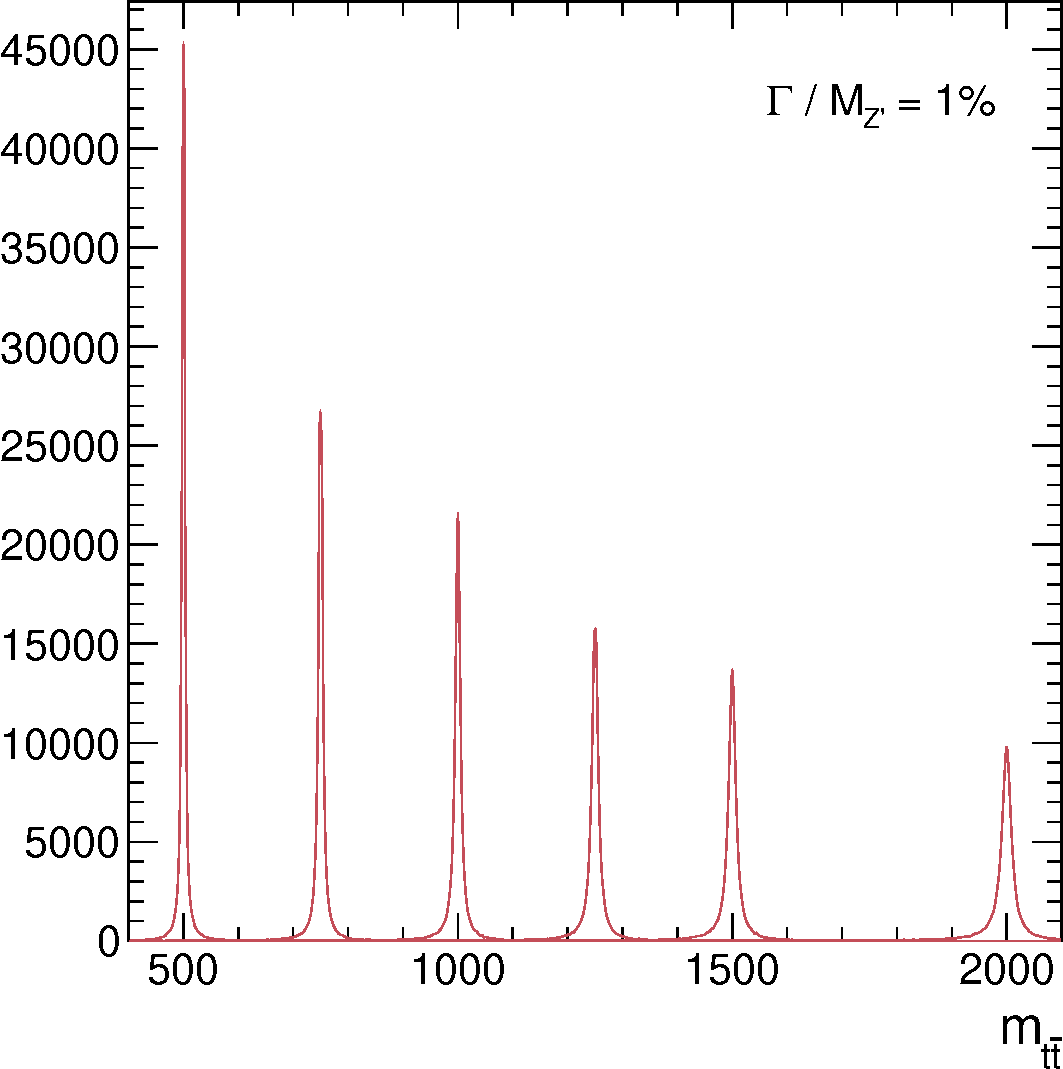
\includegraphics[width=0.33\textwidth]{chapitre7/figs/mtt_zprime_narrow_gen.pdf}} \hfill
    \subcaptionbox{\zprime large}[0.33\textwidth]{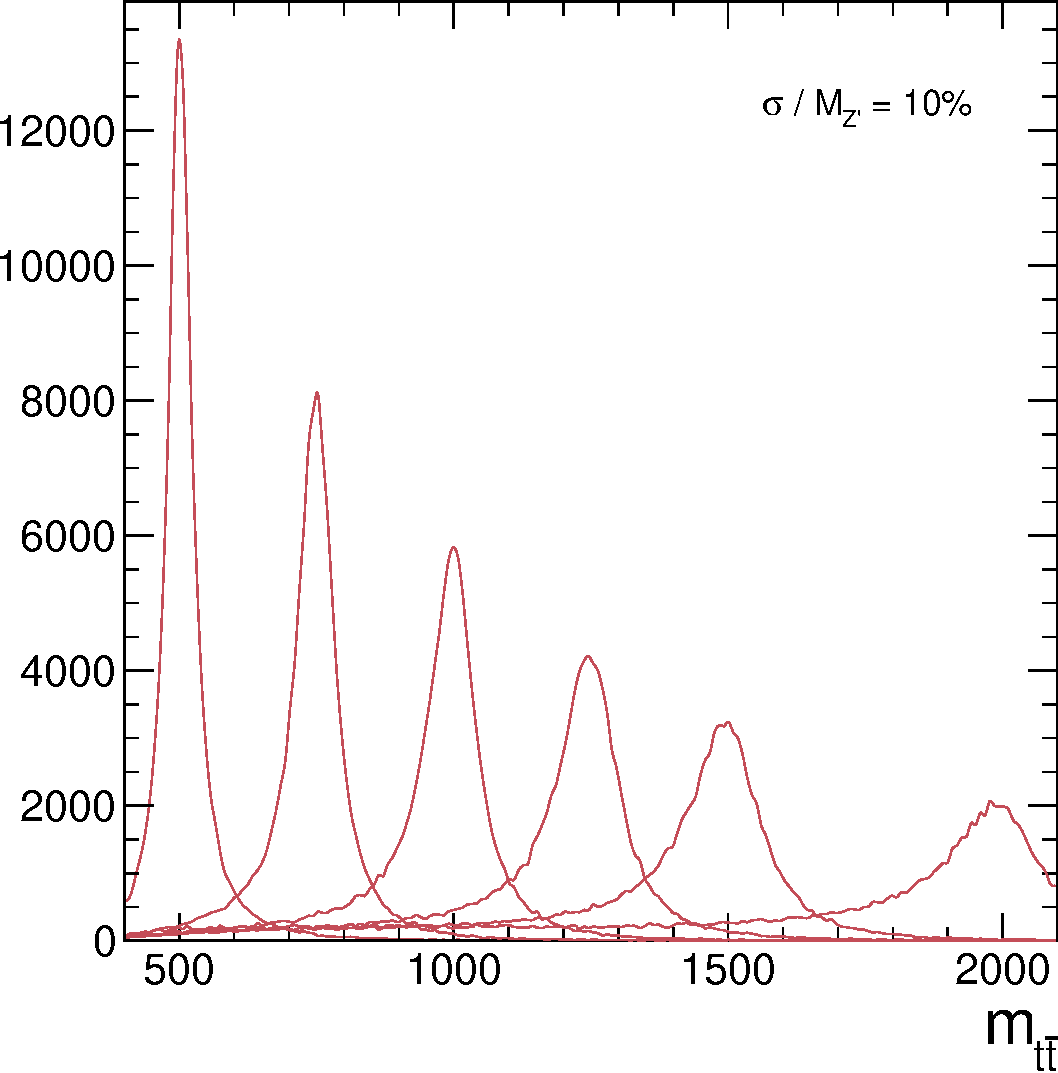
\includegraphics[width=0.33\textwidth]{chapitre7/figs/mtt_zprime_large_gen.pdf}} \hfill
    \subcaptionbox{\kkglu}[0.325\textwidth]{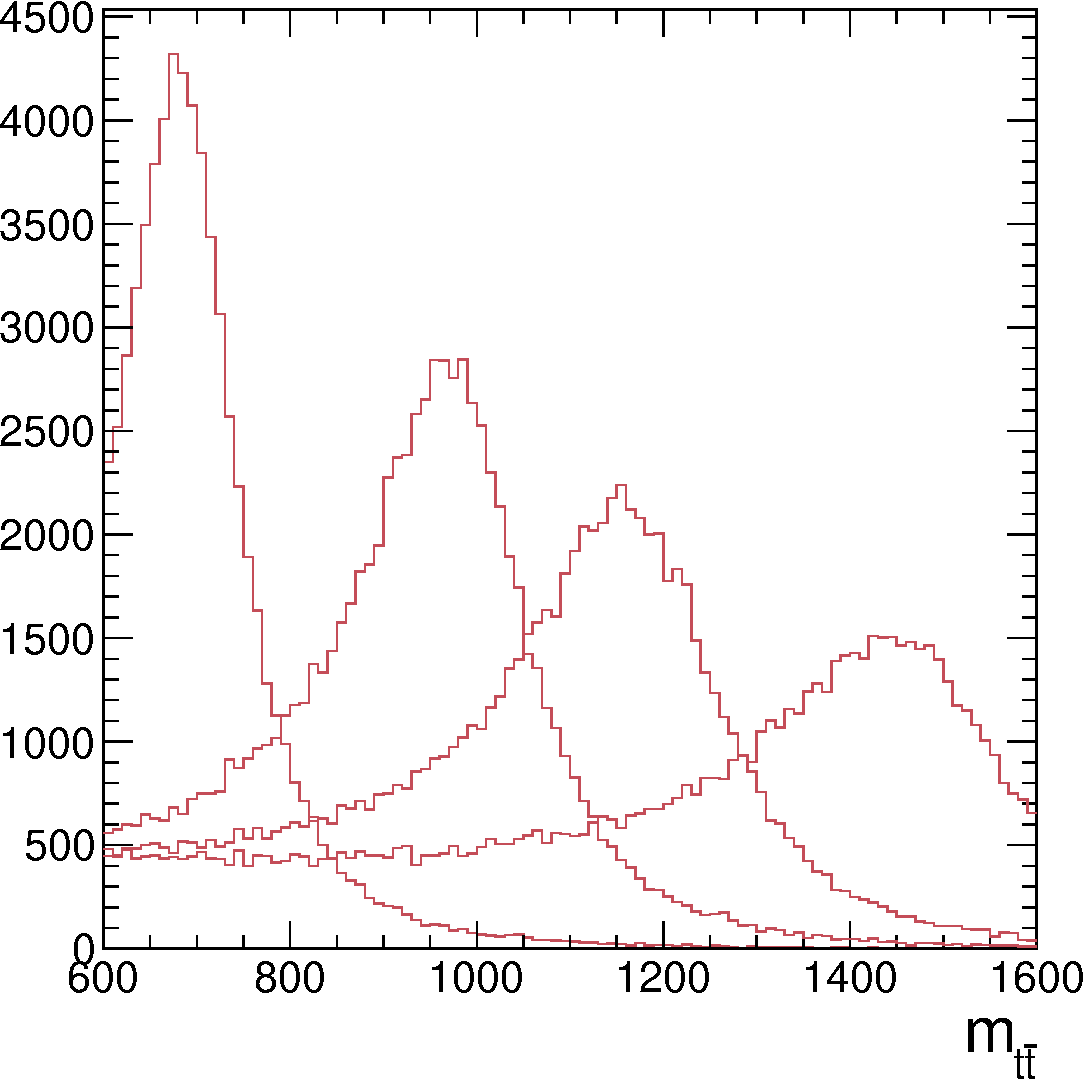
\includegraphics[width=0.325\textwidth]{chapitre7/figs/mtt_rsgluons_gen.pdf}}
    \caption{Masse invariante \ttbar pour chaque point de signal généré.}
    \label{fig:mtt_gen}
\end{figure}

\bigskip

L'analyse se concentre exclusivement sur le canal de désintégration des paires \ttbar semi-leptonique, pour plusieurs raisons :
\begin{itemize}
    \item Le rapport d'embranchement dans ce canal est \tilde\SI{44}{\%}, contre \SI{11}{\%} pour le canal di-leptonique, et \SI{45}{\%} pour le canal tout-hadronique.
    \item La présence d'un lepton constitue une signature expérimentale claire. L'avantage par rapport au canal di-leptonique, outre le rapport d'embranchement, vient de l'absence d'ambiguïté pour le choix du neutrino, améliorant la résolution de reconstruction.
    \item L'absence de neutrino dans le canal tout-hadronique est compensé par la nécessité de correctement sélectionner les 6 bons jets provenant de la désintégration \ttbar dans un environnement hadronique.
\end{itemize}

Expérimentalement, une telle désintégration se traduit par la présence d'un lepton isolé, de 4 jets, et de l'énergie transverse manquante (neutrino). Tous les processus physique du Modèle Standard produisant des états finaux similaires sont considérés comme des bruits de fond, le plus important étant la production de paires \ttbar du Modèle Standard, bruit de fond irréductible. Les autres bruits de fond considérés sont :
\begin{itemize}
    \item La production d'un boson \PW avec des jets associés (\PW + jets).
    \item La production d'un boson \PZ avec des jets associés (\PZ + jets) : un des leptons provenant de la désintégration du \PZ est mal identifié.
    \item La production d'un quark top célibataire.
\end{itemize}

\begin{table} \centering
  \begin{tabular}{@{}ccc@{}} \toprule
    Processus & Section efficace (\si{\pb}) & Luminosité équivalente (\si{\invfb}) \\ \midrule
    \ttbar & \num{234} (NNLO appr.) & \num{88.6} \\
    \PW + jets & \num{37509} (NNLO) & \num{1.5} \\
    \PZ + jets & \num{3504} (NNLO) & \num{8.7} \\
    Top célibataire (voie s) & \num{5,6} (NNLO appr.) & \num{72.0} \\
    Top célibataire (voie t) & \num{87,1} (NNLO appr.) & \num{65.4} \\
    Top célibataire (voie t\PW) & \num{22.4} (NNLO appr.) & \num{44.3} \\ \bottomrule
  \end{tabular}
  \caption{Section efficace et luminosité équivalente pour chacun des bruits de fond considérés.}
  \label{tab:backgrounds}
\end{table}

D'autres processus entrent aussi dans la composition du bruit de fond, tels que les événements multi-jets ou di-bosons (\PW{}\PW, \PZ{}\PZ, \PW{}\PZ). Après notre sélection, le nombre d'événements provenant de ces fonds est très largement minoritaire face aux autres fonds. Ils ne sont donc pas inclus dans notre analyse. Le \cref{tab:backgrounds} liste les sections efficaces de production les plus précises disponibles pour chaque bruit de fond considéré, ainsi que la luminosité équivalente disponible pour l'analyse, définie par $\mathcal{L_\text{equiv}} = N_\text{généré} \, / \, \sigma$. Ces sections efficaces sont utilisées pour normaliser les distributions des bruits de fond.

\bigskip

Afin de reproduire correctement les conditions de \pu des données, les événements dans la simulation sont pondérés de telle sorte que la distribution du nombre d'interactions par croisement de faisceau soit identique dans les données et la simulation.

\section{Sélection des événements} \label{sec:zprime_sel}

On souhaite sélectionner des événements compatibles avec la désintégration semi-leptonique de paires \ttbar, c'est-à-dire comprenant un lepton isolé, au moins 4 jets et de l'énergie transverse manquante. On applique pour cela une série de coupures afin de réduire le plus possible le bruit de fond tout en gardant un maximum d'événements de signal.

\medskip

Chaque événement est catégorisé selon la saveur du lepton. On définit ainsi le canal semi-muonique (semi-$\mu$), lorsque le lepton isolé est un muon, et le canal semi-électronique (semi-e) lorsque c'est un électron. Le tau n'est pas considéré en tant que tel, puisqu'il nécessite des techniques d'identifications et de reconstructions spéciales. Néanmoins, s'il se désintègre en électron ou en muon, l'événement est alors considéré comme un événement de signal.

\subsection{Identification des objets}

L'événement est reconstruit à l'aide de l'algorithme du \pf, décrit en détail dans le \cref{chap:reco}. Plusieurs étapes supplémentaires sont ajoutées à la reconstruction permettant de limiter les effets du \pu sur la reconstruction des jets :
\begin{itemize}
    \item On identifie les leptons isolés parmi les candidats \pf (voir \cref{sec:lepton_isolation}).
    \item On identifie ensuite les hadrons chargés provenant d'un vertex d'interaction autre que le vertex principal comme du \pu.
    \item L'agglomération des jets est ensuite effectuée avec les candidats \pf qui ne sont pas identifiés comme \pu ou leptons isolés.
\end{itemize}

Des critères de qualité sont appliqués aux muons et électrons \pf, afin de s'assurer de la qualité des objets utilisés dans l'analyse. Ces critères sont détaillés dans la suite de cette section. La sélection sera elle détaillée dans la prochaine section. Pour chaque saveur, deux jeux de critères sont définis : une sélection lâche, qui servira pour effectuer un veto sur la présence de leptons additionnels, et une sélection forte, utilisée pour sélectionner le lepton principal.

\subsubsection{Muons} \label{sec:sel_muon}

Afin d'être identifié comme lâche, un muon doit passer les coupures suivantes :
\begin{itemize}
    \item Le muon doit être reconstruit avec l'algorithme du \pf, et être soit \emph{tracker} ou global (voir \cref{sec:muon_reco}).
    \item L'isolation relative $I_{\Pmu}^\text{corrigé}$ doit être inférieure à \SI{20}{\%}.
    \item L'impulsion transverse doit être supérieure à \SI{10}{\GeV}, et $\aeta < \num{2.5}$.
\end{itemize}

\begin{figure}[tbp] \centering
    \subcaptionbox{\label{fig:muon_id_eff}}[0.48\textwidth]{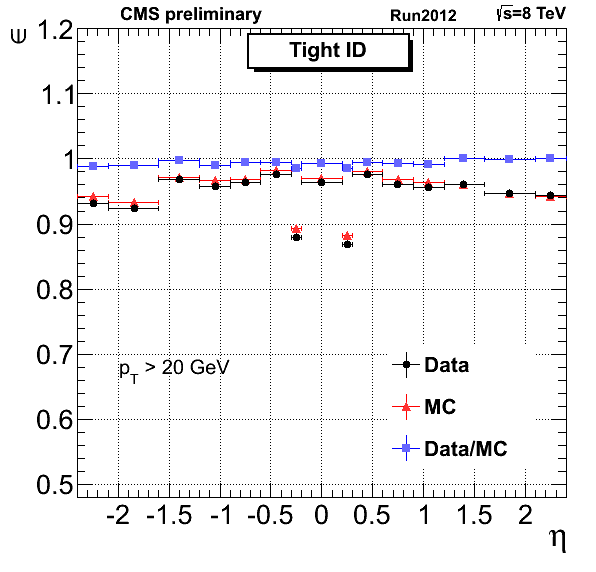
\includegraphics[width=0.48\textwidth]{chapitre7/figs/muon_id_efficiency.png}} \hfill
    \subcaptionbox{\label{fig:muon_iso_eff}}[0.48\textwidth]{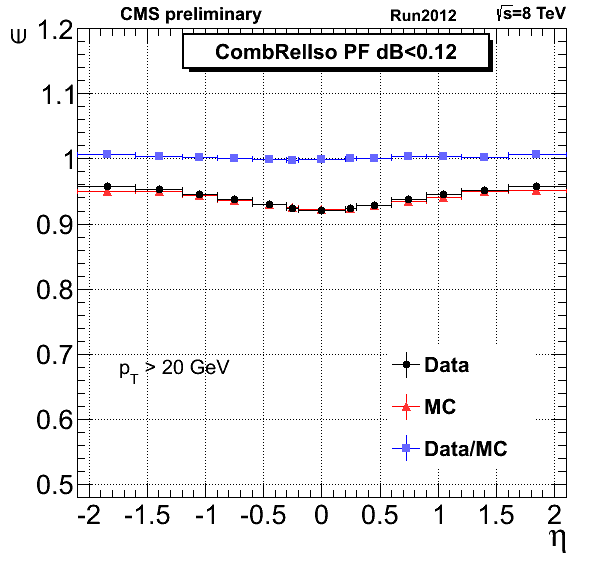
\includegraphics[width=0.48\textwidth]{chapitre7/figs/muon_iso_efficiency.png}}
    \caption{Efficacité de la sélection appliquée aux muons (hors isolation) (\subref{fig:muon_id_eff}) ainsi que l'isolation (\subref{fig:muon_iso_eff}) en fonction de \aeta, pour les données 2012 (noir) ainsi que la simulation (rouge). Pour les données, l'efficacité est calculée à l'aide d'une méthode \emph{tag and probe} sur des événements $\PZ \rightarrow \Pmuon\APmuon$.}
\end{figure}

En plus de ces coupures, on identifie un muon de qualité (\emph{tight}) s'il vérifie les critères suivants :
\begin{itemize}
  \item Le muon doit être reconstruit avec l'algorithme du \pf, et être un muon global.
  \item L'isolation relative $I_{\Pmu}^\text{corrigé}$ (voir \cref{sec:lepton_isolation}) doit être inférieure à \SI{12}{\%}.
  \item La valeur du $\chi^2$ de l'ajustement global de la trace du muon divisé par le nombre de degrés de liberté de l'ajustement doit être inférieure à \num{10}.
  \item Le nombre de \emph{hits} laissés par le muons dans les couches du trajectographe doit être au moins égal à 5, afin d'assurer une mesure précise de l'impulsion transverse.
  \item L'ajustement global de la trace doit inclure au moins un \emph{hit} dans les chambres à muons.
  \item La distance longitudinale de la trace par rapport au vertex primaire $d_Z$ doit être inférieure à \SI{0.5}{\cm}.
  \item La distance du paramètre d'impact transverse par rapport au vertex primaire $d_0$ doit être inférieure à \SI{0.2}{\cm}.
  \item L'impulsion transverse du muon doit être supérieure à \SI{26}{\GeV}, et $\aeta < \num{2.1}$.
\end{itemize}

La \cref{fig:muon_id_eff} présente l'efficacité de cette sélection, qui varie entre \num{88} et \SI{98}{\%}. L'efficacité de l'isolation, évaluée sur les données après sélection, est présentée sur la \cref{fig:muon_iso_eff}, et varie entre \num{92} et \SI{96}{\%}. Pour les données, l'efficacité est calculée à l'aide d'une méthode \emph{tag and probe} sur des événements $\PZ \rightarrow \Pmuon\APmuon$.

\subsubsection{Électrons} \label{sec:sel_electron}

De façon analogue aux muons, on définit également deux jeux de critères pour identifier les électrons, détaillés dans le tableau ci-dessous.

\begin{table}[htbp] \centering
  \begin{tabular}{@{}ccc@{}} \toprule

  Variable & Électron lâche & Électron de qualité \\ \midrule
  & \multicolumn{2}{c}{électron \pf} \\
  $\Delta \eta_{IN}$ & \num{< 0.007} & \num{< 0.004} \\
  $\Delta \phi_{IN}$ & \num{< 0.8} & \num{< 0.03} \\
  $\sigma_{i\eta i\eta}$ & \num{< 0.01} & \num{< 0.01} \\
  $ H / E $ & \num{< 0.15} & \num{< 0.12} \\
  $d_0$ & \num{< 0.04} & \num{< 0.02} \\
  $d_Z$ & \num{< 0.2} & \num{< 0.1} \\
  $1 / E - 1 / P$ & - & < 0.05 \\
  \pt & \SI{>= 20}{\GeV} & \SI{>= 30}{\GeV} \\
  $\aeta$ & \num{< 2.5} & \num{< 2.5} \\
  $I_{\Pe}^\text{corrigé}$ (voir \cref{sec:lepton_isolation}) & \num{< 0.15} & \num{< 0.10} \\
  \bottomrule

  \end{tabular}
\end{table}

$\Delta \eta_{IN}$ est la différence entre $\eta$ de l'agrégat calorimétrique et $\eta$ de la trace de l'électron, $\Delta \phi_{IN}$ entre la différence entre $\phi$ de l'agrégat calorimétrique et $\phi$ de la trace de l'électron, et $\sigma_{i\eta i\eta}$ et $H / E$ sont définis dans la \cref{sec:jetmet_sel}. L'efficacité de la sélection d'un électron de qualité est présentée dans la \cref{fig:electron_id_eff}, et varie entre \num{75} et \SI{90}{\percent} pour les électrons considérés par l'analyse. Pour les données, l'efficacité est calculée à l'aide d'une méthode \emph{tag and probe} sur des événements $\PZ \rightarrow \Pelectron\APelectron$.

\begin{figure}[thbp]
  \centering
  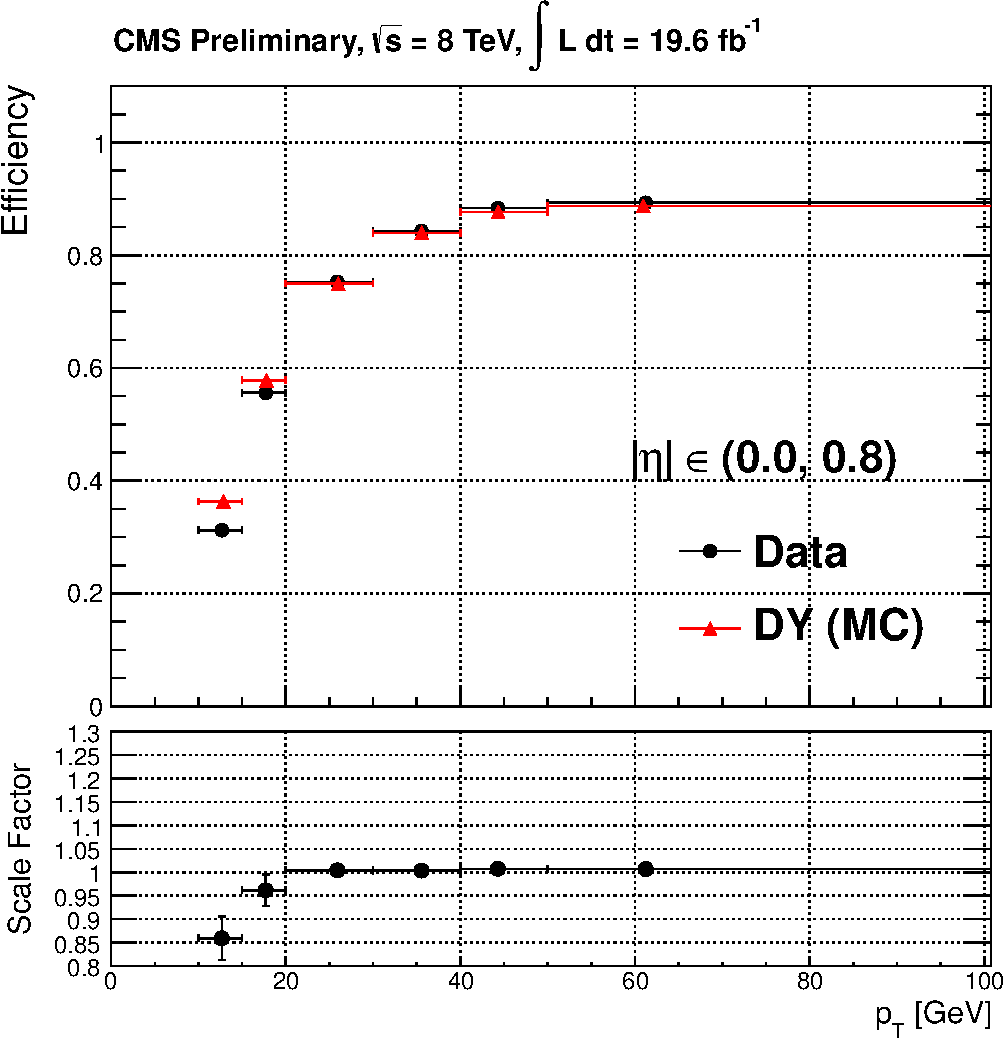
\includegraphics[width=0.53\textwidth]{chapitre7/figs/electron_id_eff.pdf}
  \caption{Comparaison entre l'efficacité de la sélection d'un électron de qualité pour la simulation (rouge) et les données 2012 (noir). Le ratio entre données et simulation est présenté en dessous de la figure. Pour les données, l'efficacité est calculée à l'aide d'une méthode \emph{tag and probe} sur des événements $\PZ \rightarrow \Pelectron\APelectron$.}
  \label{fig:electron_id_eff}
\end{figure}

\subsubsection{Jets}

Les jets sont reconstruits à l'aide de l'algorithme anti-$k_T$, avec une largeur de cône $R = \num{0.5}$ (voir \cref{sec:jet_reco}). Toutes les particules \pf n'étant ni des leptons isolés, ni du \pu, sont utilisées dans l'agglomération des jets. Les corrections de niveaux 1, 2 et 3 sont appliquées, ainsi que les corrections résiduelles sur les données uniquement (plus de détails dans les \cref{sec:jec_l1,sec:jec_l2l3,sec:jec_res}).

On a évoqué rapidement dans le \cref{chap:jetmet} que la résolution des jets sur la simulation était meilleure que celle des jets reconstruits sur les données. On applique une série de corrections afin de dégrader la résolution des jets sur la simulation, afin de correspondre mieux à celle des données. L'impulsion transverse des jets est corrigée par un facteur $C$, défini par :
\begin{align*}
  C &= \max\left(0, 1 + \left[ 1 - \frac{\pt^\text{gen}}{\pt^\text{jet}} \right] \, f(\pt, \eta)\right)
\end{align*}
où $\pt^\text{jet}$ est l'impulsion transverse du jet, $\pt^\text{gen}$ est l'impulsion transverse du jet généré, et $f(\pt, \eta)$ un facteur de correction permettant de dégrader la résolution des jets. Les corrections en énergie et en résolution des jets sont propagées à l'énergie transverse manquante (voir \cref{sec:jetmet_sel}, \cpageref{page:met_propagation} pour plus de détails).

L'algorithme utilisé pour l'étiquetage des jets de \Pbottom est présenté en détail \cref{sec:b_tagging}. Afin d'éliminer les jets provenant des bruits des détecteurs, une sélection lâche est appliquée, demandant que la fraction d'énergie hadronique du jet soit inférieure à \SI{99}{\percent}, et que le nombre de particules constituant le jet soit au moins égal à 2. Cette sélection a une efficacité supérieure à \SI{99}{\%}.

\subsubsection{Énergie transverse manquante}

L'énergie transverse manquante est reconstruite à l'aide de toutes les particules \pf de l'événement, comme décrit \cref{sec:met}. Toutes les corrections appliquées aux jets sont propagées à l'énergie transverse manquante.

\medskip

La distribution de l'énergie transverse manquante est isotrope en $\phi$ à cause d'une symétrie de rotation des collisions autour de l'axe $z$. Il est cependant observé sur les données qu'après reconstruction, la distribution de $\phi$ de l'énergie transverse manquante n'est pas constante, mais présente une oscillation sinusoïdale de période \tilde$\num{2}\pi$. Cette oscillation peut avoir plusieurs causes, telles qu'une réponse anisotropique des détecteurs, des cellules calorimétriques inactives, un mauvais alignement des détecteurs, ainsi qu'un décalage du point d'interaction. On corrige cet effet, préjudiciable pour la reconstruction de la masse invariante, en décalant l'origine des coordonnées $x$ et $y$ :
\begin{align*}
  \METx &= \METx^\text{non corrigé} + c_x\\
  \METy &= \METy^\text{non corrigé} + c_y
\end{align*}
où $c_y$ et $c_y$ sont les facteurs de corrections, dérivées centralement par la collaboration. L'effet de cette correction est visible dans la \cref{fig:met_phi}.

\bigskip

\begin{figure}[tbp] \centering
    \subcaptionbox{\label{fig:met_phi}}[0.48\textwidth]{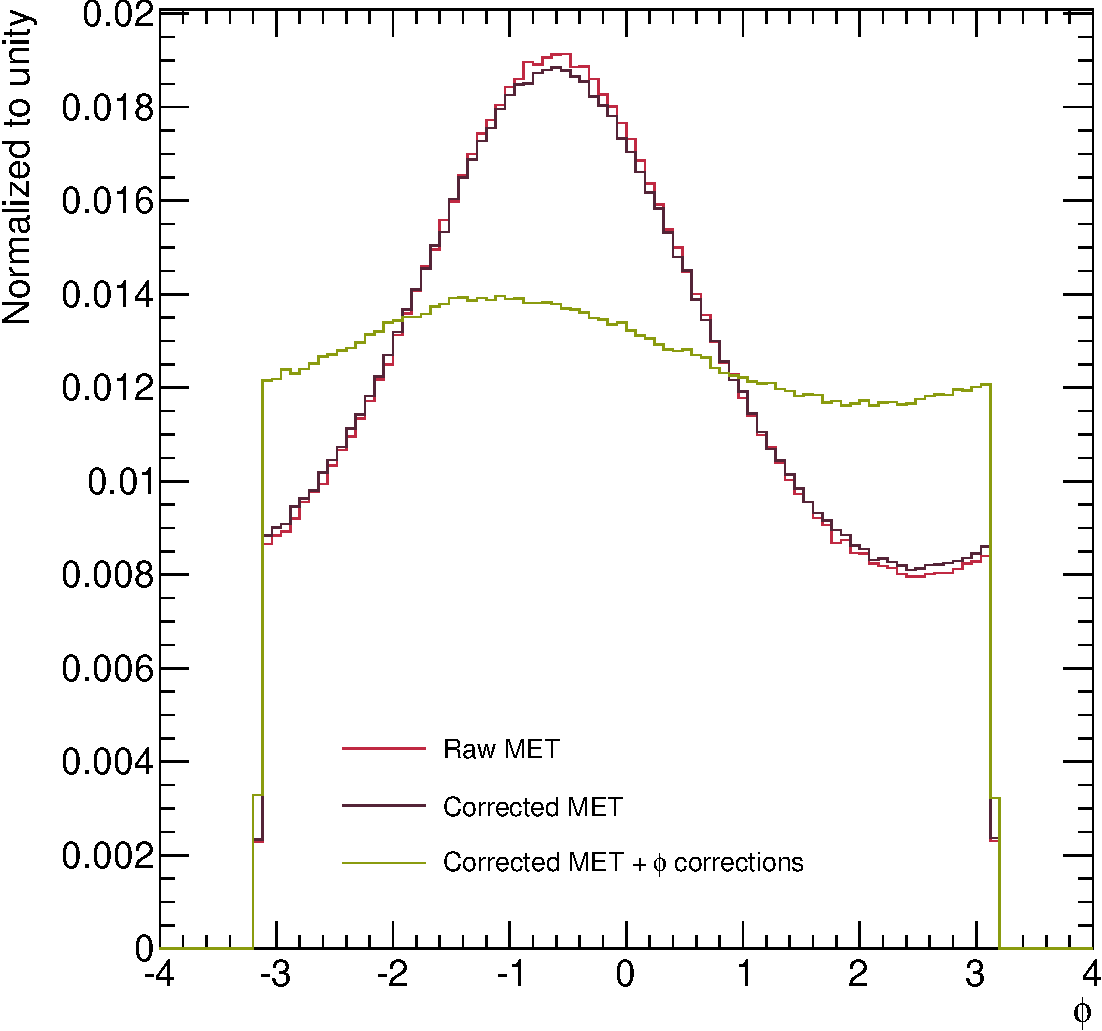
\includegraphics[width=0.48\textwidth]{chapitre7/figs/met_phi_corrections.pdf}}
    \subcaptionbox{\label{fig:met_cleaning}}[0.48\textwidth]{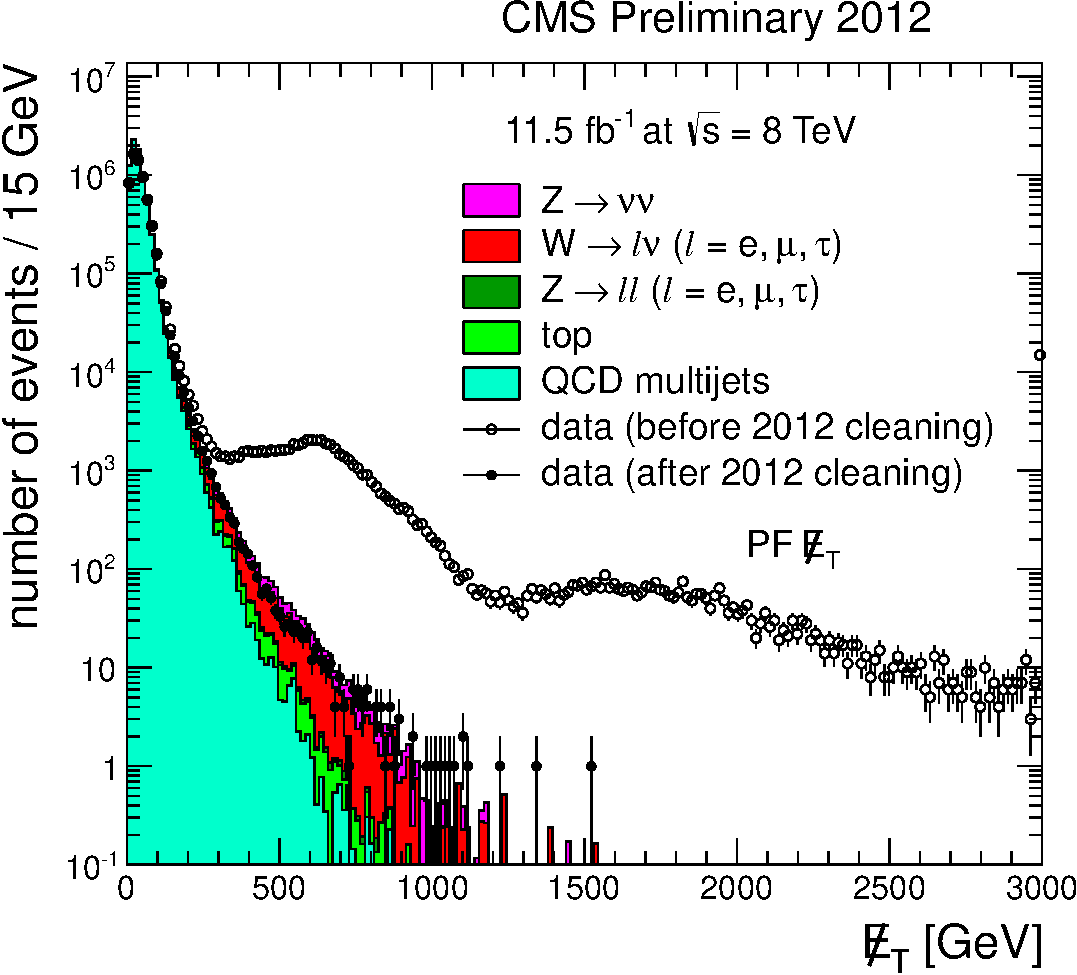
\includegraphics[width=0.48\textwidth]{chapitre7/figs/met_cleaning.pdf}}
    \caption{(\subref{fig:met_phi}) Oscillation en $\phi$ de l'énergie transverse manquante, sans aucune correction (\rouge), après propagation de la correction en énergie des jets (\violet), et après corrections dédiées à l'oscillation en $\phi$ (\vertc). (\subref{fig:met_cleaning}) Effet du nettoyage des données 2012 sur l'énergie transverse manquante.}
\end{figure}

Un autre effet à prendre en compte est la présence, dans les données, de rares événements qui contiennent une quantité anormalement grande d'énergie transverse manquante. Cette fausse énergie manquante a plusieurs origines :
\begin{itemize}
  \item Des collisions peuvent se produire entre les protons des faisceaux et le gaz résiduel dans les tubes transportant les protons. Dans de rare cas, ces particules peuvent traverser le détecteur, et ainsi apparaître comme de l'énergie transverse manquante.
  \item Du bruit anormal dans le HCAL, causé par des problèmes de lecture des photodiodes, peut provoquer de la fausse énergie manquante jusqu'à l'échelle du \si{\TeV}.
  \item Il arrive que le système de synchronisation temporelle du HCAL, utilisant un faisceau laser, se déclenche en même temps qu'une collision. Ce phénomène est extrêmement rare (en 2011, 216 événements ont été identifiés), mais peut causer de grandes valeurs d'énergie transverse manquante.
  \item Certains cristaux du ECAL sont connus pour être très bruyants. Ils sont donc ignorés lors de la reconstruction. Beaucoup d'énergie peut ainsi être manquée lorsqu'une particule interagit avec ces cristaux, provoquant une source anormale d'énergie transverse manquante.
\end{itemize}

Des filtres ont ainsi été développés afin de supprimer les événements contenant de la fausse énergie transverse manquante. On peut voir sur la \cref{fig:met_cleaning} l'effet d'un tel nettoyage : avec l'utilisation des filtres, la queue de la distribution, causée par de la fausse \met, disparaît.

\subsection{Sélection des événements}

% Les données collectées par CMS sont classées dans plusieurs ensembles selon les chemins de déclenchements activés. Pour cette analyse, la totalité des données collectées en 2012 est utilisée, correspond à une luminosité intégrée totale de \SI{19.6}{\invfb}. Deux ensembles de données particuliers sont utilisés :
% \begin{itemize}
%   \item L'ensemble \emph{SingleMu}, pour le canal semi-muonique.
%   \item L'ensemble \emph{SingleElectron}, pour le canal semi-électronique.
% \end{itemize}

% On souhaite sélectionner des événements ayant un lepton isolé ainsi qu'au moins 4 jets. Afin de baisser au maximum les seuils en impulsion transverse sur les chemins de déclenchements, on demande aux données d'avoir activé les chemins de déclenchements demandant un lepton isolé et au moins 3 jets centraux ($\aeta < \num{2.5}$). On arrive ainsi à obtenir

On considère pour l'analyse la totalité des données collectées par CMS en 2012 (\SI{19.6}{\invfb}), et plus particulièrement les événements ayant activé des chemins de déclenchement demandant un muon isolé d'au moins \SI{17}{\GeV} ou un électron isolé d'au moins \SI{25}{\GeV}, accompagnés d'au moins trois jets d'au moins \SI{30}{\GeV}. Les conditions de prises de données ayant changé pendant l'année 2012, les seuils sur l'impulsion transverse des jets des chemins de déclenchement ont dû être ajustés. Ainsi, on demande au final 4 chemins différents pour le canal semi-muonique et 4 pour le canal semi-électronique. Dans les figures qui suivent, ces chemins ont pour alias respectivement \texttt{HLT\_MuX} (\texttt{HLT\_EleX}), X = A, B, C et D.

\bigskip

La sélection appliquée pour chaque canal est identique, excepté la saveur du lepton demandé. Pour être sélectionné, une événement doit contenir :

\begin{itemize}
  \item Exactement un muon (électron) de qualité, suivant les critères définis \cref{sec:sel_muon} (\cref{sec:sel_electron}). L'événement est rejeté s'il contient en plus un ou plusieurs leptons vérifiant les conditions lâches.
  \item Au moins 4 jets avec $\aeta < \num{2.4}$ et $\pt > 70\,/\,50\,/\,30\,/\,\SI{30}{\GeV}$. Cette coupure étagée permet d'optimiser le rapport signal sur bruit.
  \item Au moins 1 jet étiqueté \Pbottom.
  \item $\met > \SI{20}{\GeV}$. Cette coupure permet d'éliminer une majorité du fond multi-jets.
\end{itemize}

Les événements passant la sélection sont ensuite classés en 4 catégories, selon la saveur du lepton et le nombre de jets étiquetés \Pbottom :
\begin{center}
  \begin{tabular}{c} \toprule
    muon \\
    électron \\ \bottomrule
  \end{tabular} \qquad $\otimes$ \qquad
  \begin{tabular}{c} \toprule
    Exactement 1 jet étiqueté \Pbottom \\
    Au moins 2 jets étiquetés \Pbottom \\ \bottomrule
  \end{tabular}
\end{center}

\section{Performances de la sélection}

\subsection{Efficacité des chemins de déclenchement} \label{sec:zp_eff_hlt}

\begin{figure}[tbp] \centering
    \subcaptionbox{Canal semi-muonique}[0.48\textwidth]{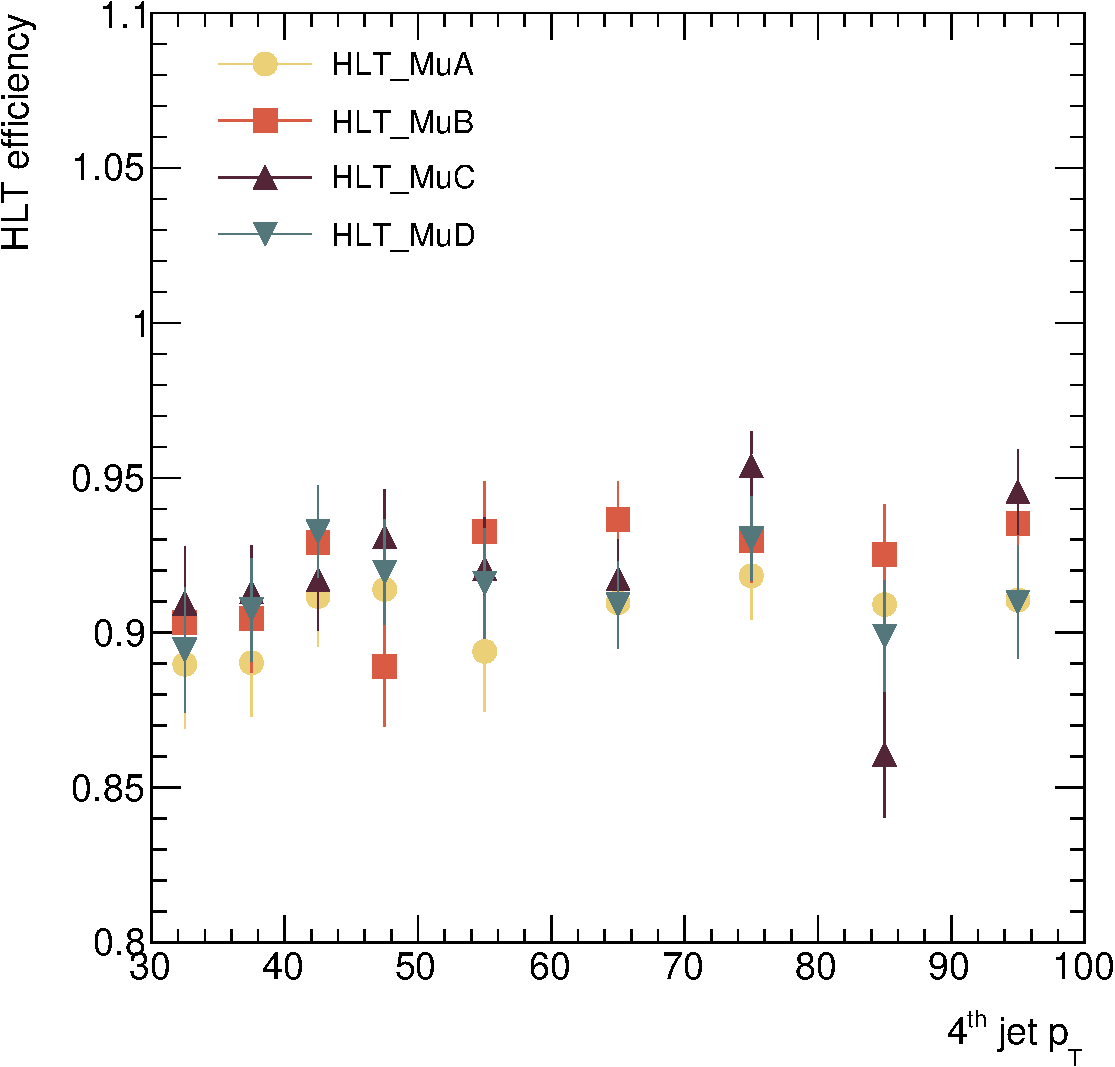
\includegraphics[width=0.48\textwidth]{chapitre7/figs/HLT/HLTturnon_mu_fourthJet_zoom.pdf}}
    \subcaptionbox{Canal semi-électronique}[0.48\textwidth]{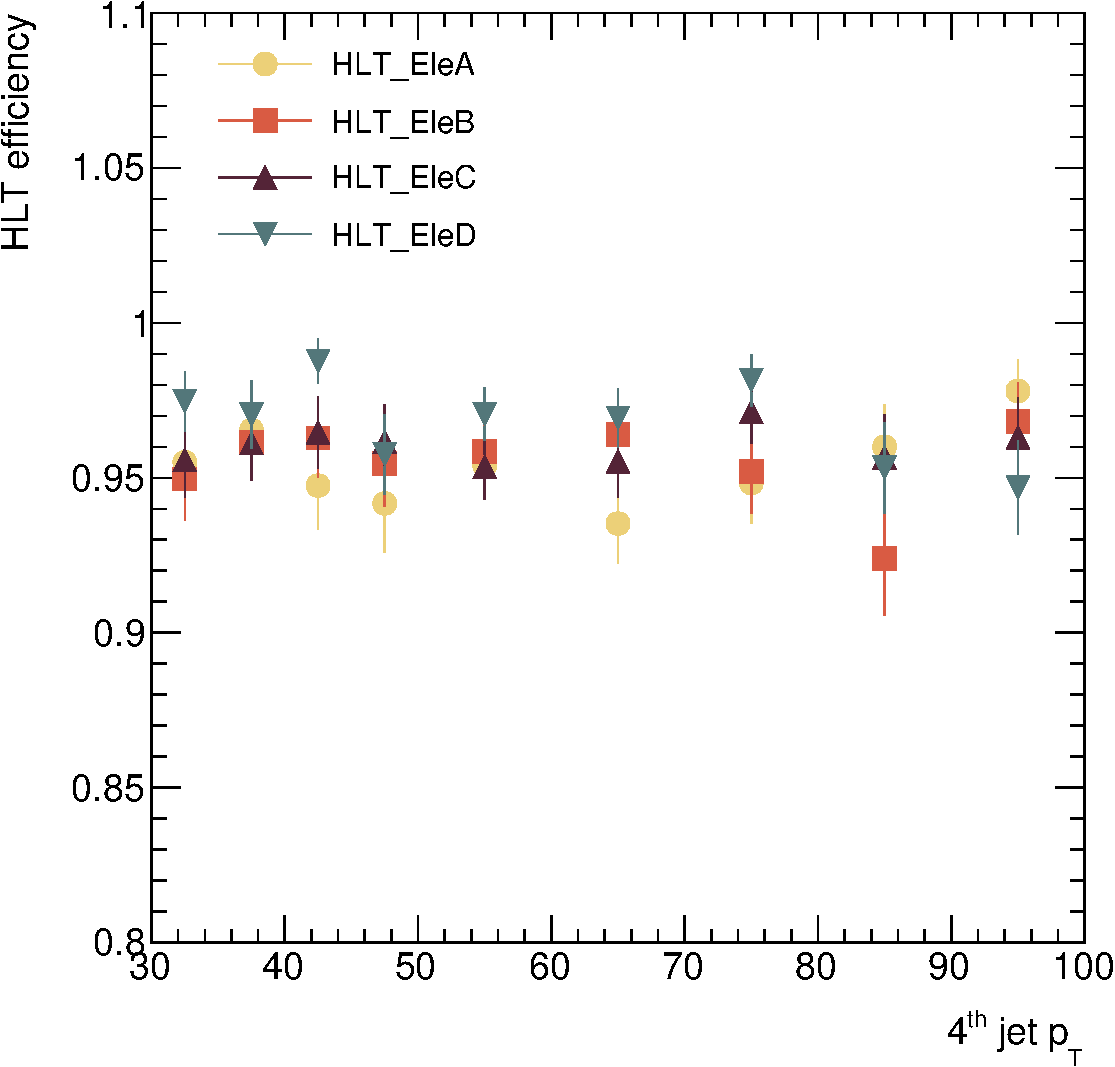
\includegraphics[width=0.48\textwidth]{chapitre7/figs/HLT/HLTturnon_el_fourthJet_zoom.pdf}}
    \caption{Efficacité des chemins de déclenchement en fonction de l'impulsion transverse du quatrième jet.}
    \label{fig:trig_eff}
\end{figure}


\begin{table}[p!] \centering \footnotesize
\begin{tabular}{@{}ccccc@{}} \toprule
 & \texttt{HLT\_MuA} & \texttt{HLT\_MuB} & \texttt{HLT\_MuC} & \texttt{HLT\_MuD} \\ \midrule
$\epsilon$ ($\mzp = \SI{750}{\GeV}$)& \num{0.909\pm 0.006} & \num{0.909\pm 0.006}& \num{0.917\pm 0.006} & \num{0.909\pm 0.006} \\
$\epsilon$ ($\mzp = \SI{1000}{\GeV}$)& \num{0.899\pm 0.007} & \num{0.916\pm 0.006} & \num{0.928\pm 0.006} & \num{0.918\pm 0.006} \\
$\epsilon$ ($\mzp = \SI{1250}{\GeV}$)& \num{0.889\pm 0.008} & \num{0.908\pm 0.007} & \num{0.904\pm 0.007} & \num{0.908\pm 0.007} \\
$\epsilon$ ($\mzp = \SI{1500}{\GeV}$)& \num{0.900\pm 0.008} & \num{0.908\pm 0.008} & \num{0.904\pm 0.008} & \num{0.930\pm 0.007} \\
$\epsilon$ (\ttbar)& \num{0.891\pm 0.006} & \num{0.912\pm 0.006} & \num{0.915\pm 0.006} & \num{0.929\pm 0.006} \\ \hline
\end{tabular}
\caption{Efficacités des chemins de déclenchement pour le canal semi-muonique, et au moins 2 jets étiquetés \Pbottom.}
\label{tab:HLT_mu_eff_2btag}
\end{table}

\begin{table}[p!] \centering \footnotesize
\begin{tabular}{@{}ccccc@{}} \toprule
 & \texttt{HLT\_MuA} & \texttt{HLT\_MuB} & \texttt{HLT\_MuC} & \texttt{HLT\_MuD} \\ \midrule
$\epsilon$ ($\mzp = \SI{750}{\GeV}$)& \num{0.902\pm 0.007} & \num{0.920\pm 0.006} & \num{0.921\pm 0.006} & \num{0.913\pm0.007} \\
$\epsilon$ ($\mzp = \SI{1000}{\GeV}$)& \num{0.897\pm 0.007} & \num{0.918\pm 0.006} & \num{0.917\pm 0.006} & \num{0.922\pm 0.006} \\
$\epsilon$ ($\mzp = \SI{1250}{\GeV}$)& \num{0.899\pm 0.008} & \num{0.904\pm 0.007} & \num{0.902\pm 0.007} & \num{0.919\pm 0.006} \\
$\epsilon$ ($\mzp = \SI{1500}{\GeV}$)& \num{0.902\pm 0.007} & \num{0.910\pm 0.008} & \num{0.919\pm 0.007} & \num{0.925\pm 0.007} \\
$\epsilon$ (\ttbar)& \num{0.883\pm 0.006} & \num{0.915\pm 0.006} & \num{0.913\pm 0.006} & \num{0.919\pm 0.006} \\ \hline
\end{tabular}
\caption{Efficacités des chemins de déclenchement pour le canal semi-muonique, et exactement 1 jet étiqueté \Pbottom.}
\label{tab:HLT_mu_eff_1btag}
\end{table}

\begin{table}[p!] \centering \footnotesize
\begin{tabular}{@{}ccccc@{}} \toprule
 & \texttt{HLT\_EleA} & \texttt{HLT\_EleB} & \texttt{HLT\_EleC} & \texttt{HLT\_EleD} \\ \midrule
$\epsilon$ ($\mzp = \SI{750}{\GeV}$)& \num{0.955\pm 0.005} & \num{0.956\pm 0.005} & \num{0.958\pm 0.005} & \num{0.966\pm0.005} \\
$\epsilon$ ($\mzp = \SI{1000}{\GeV}$)& \num{0.968\pm 0.004} & \num{0.962\pm 0.005} & \num{0.966\pm 0.004} & \num{0.975\pm 0.004} \\
$\epsilon$ ($\mzp = \SI{1250}{\GeV}$)& \num{0.958\pm 0.005} & \num{0.957\pm 0.005} & \num{0.958\pm 0.005} & \num{0.964\pm 0.005} \\
$\epsilon$ ($\mzp = \SI{1500}{\GeV}$)& \num{0.955\pm 0.006} & \num{0.954\pm 0.006} & \num{0.950\pm 0.006} & \num{0.963\pm 0.005} \\
$\epsilon$ (\ttbar)& \num{0.956\pm 0.005} & \num{0.960\pm 0.004} & \num{0.958\pm 0.004} & \num{0.973\pm 0.004}  \\ \hline
\end{tabular}
\caption{Efficacités des chemins de déclenchement pour le canal semi-électronique, et au moins 2 jets étiquetés \Pbottom.}
\label{tab:HLT_el_eff_2btag}
\end{table}

\begin{table}[p!] \centering \footnotesize
\begin{tabular}{@{}ccccc@{}} \toprule
 & \texttt{HLT\_EleA} & \texttt{HLT\_EleB} & \texttt{HLT\_EleC} & \texttt{HLT\_EleD} \\ \midrule
$\epsilon$ ($\mzp = \SI{750}{\GeV}$)& \num{0.949\pm 0.005} & \num{0.954\pm 0.005} & \num{0.960\pm 0.005} & \num{0.976\pm0.004} \\
$\epsilon$ ($\mzp = \SI{1000}{\GeV}$)& \num{0.950\pm 0.005} & \num{0.962\pm 0.005} & \num{0.957\pm 0.005} & \num{0.960\pm 0.005} \\
$\epsilon$ ($\mzp = \SI{1250}{\GeV}$)& \num{0.958\pm 0.005} & \num{0.947\pm 0.005} & \num{0.962\pm 0.005} & \num{0.963\pm 0.004} \\
$\epsilon$ ($\mzp = \SI{1500}{\GeV}$)& \num{0.945\pm 0.005} & \num{0.932\pm 0.006} & \num{0.946\pm 0.006} & \num{0.960\pm 0.005} \\
$\epsilon$ (\ttbar)& \num{0.956\pm 0.005} & \num{0.954\pm 0.004} & \num{0.957\pm 0.004} & \num{0.968\pm 0.004} \\ \hline
\end{tabular}
\caption{Efficacités des chemins de déclenchement pour le canal semi-électronique, et exactement 1 jet étiqueté \Pbottom.}
\label{tab:HLT_el_eff_1btag}
\end{table}

Afin d'estimer au mieux l'efficacité des chemins de déclenchement utilisés par l'analyse, chaque chemin a été simulé individuellement pour chaque point de signal considéré. Il est ainsi possible d'évaluer l'efficacité de chaque chemin.

Un facteur de correction additionnel est appliqué à chaque efficacité pour tenir compte des différences de performances entre la simulation des chemins et les données. Ces facteurs sont disponibles pour toutes les analyses, et son calculés avec une sélection identique pour les leptons, mais légèrement différente (plus lâche) pour les jets. La \cref{fig:trig_eff} présente un exemple de courbes d'efficacités pour les chemins de déclenchement utilisés dans l'analyse. On peut constater que les coupures appliquées sur les jets permettent d'être sur le plateau d'efficacité des chemins. On peut ainsi utiliser une efficacité non dépendante de l'impulsion transverse des objets. Les \cref{tab:HLT_mu_eff_2btag,tab:HLT_mu_eff_1btag,tab:HLT_el_eff_2btag,tab:HLT_el_eff_1btag} résument les efficacités obtenues pour chaque chemin de déclenchement, pour chacune des catégories de l'analyse et séparément pour chaque masse de signal et le bruit de fond \ttbar : l'efficacité de déclenchement n'est pas dépendante de la masse du \zprime, et  est compatible entre \zprime et \ttbar. Pour le canal semi-muonique, l'efficacité moyenne est d'environ \SI{90}{\%}, et environ \SI{95}{\%} pour le canal semi-électronique.

% \begin{figure}[tbp] \centering
%     \subcaptionbox{Canal semi-muonique}[0.48\textwidth]{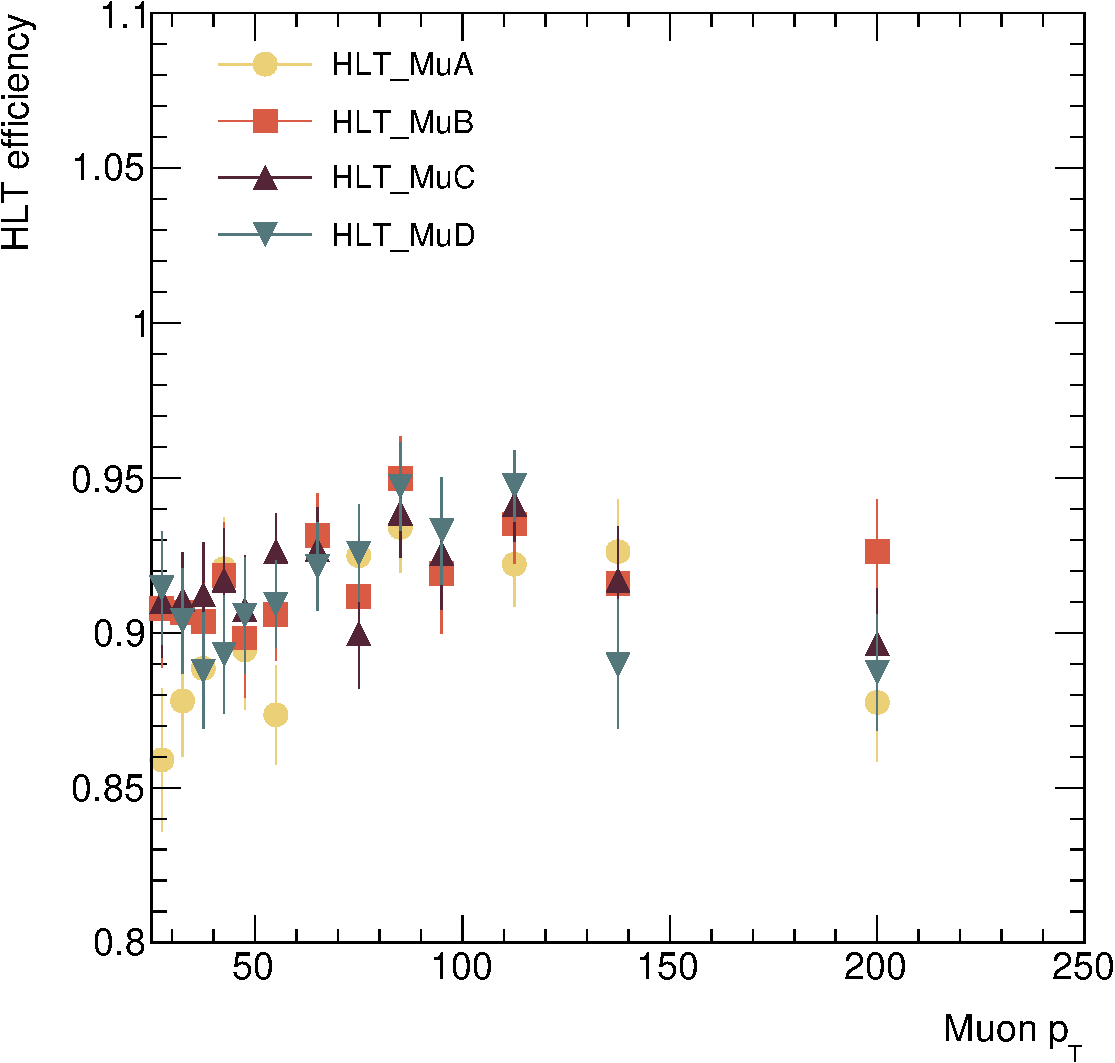
\includegraphics[width=0.48\textwidth]{chapitre7/figs/HLT/HLTturnon_mu_lepton_zoom.pdf}}
%     \subcaptionbox{Canal semi-électronique}[0.48\textwidth]{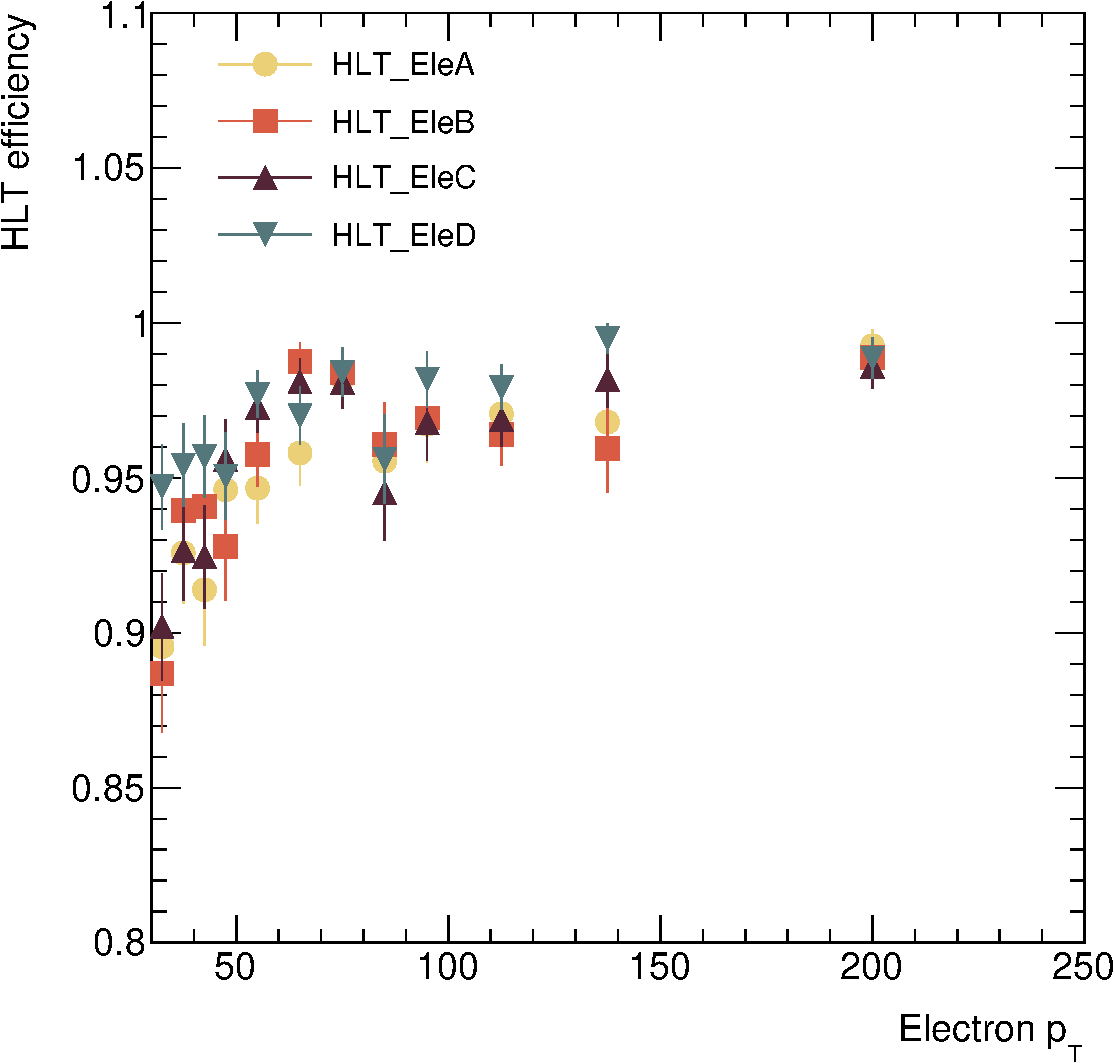
\includegraphics[width=0.48\textwidth]{chapitre7/figs/HLT/HLTturnon_el_lepton_zoom.pdf}}
%     \caption{Efficacité des chemins de déclenchements en fonction de l'impulsion transverse du lepton.}
%     \label{fig:trig_eff_leptons}
% \end{figure}

% \begin{figure}[tbp] \centering
%     \subcaptionbox{\ordinalnum{1} jet}[0.48\textwidth]{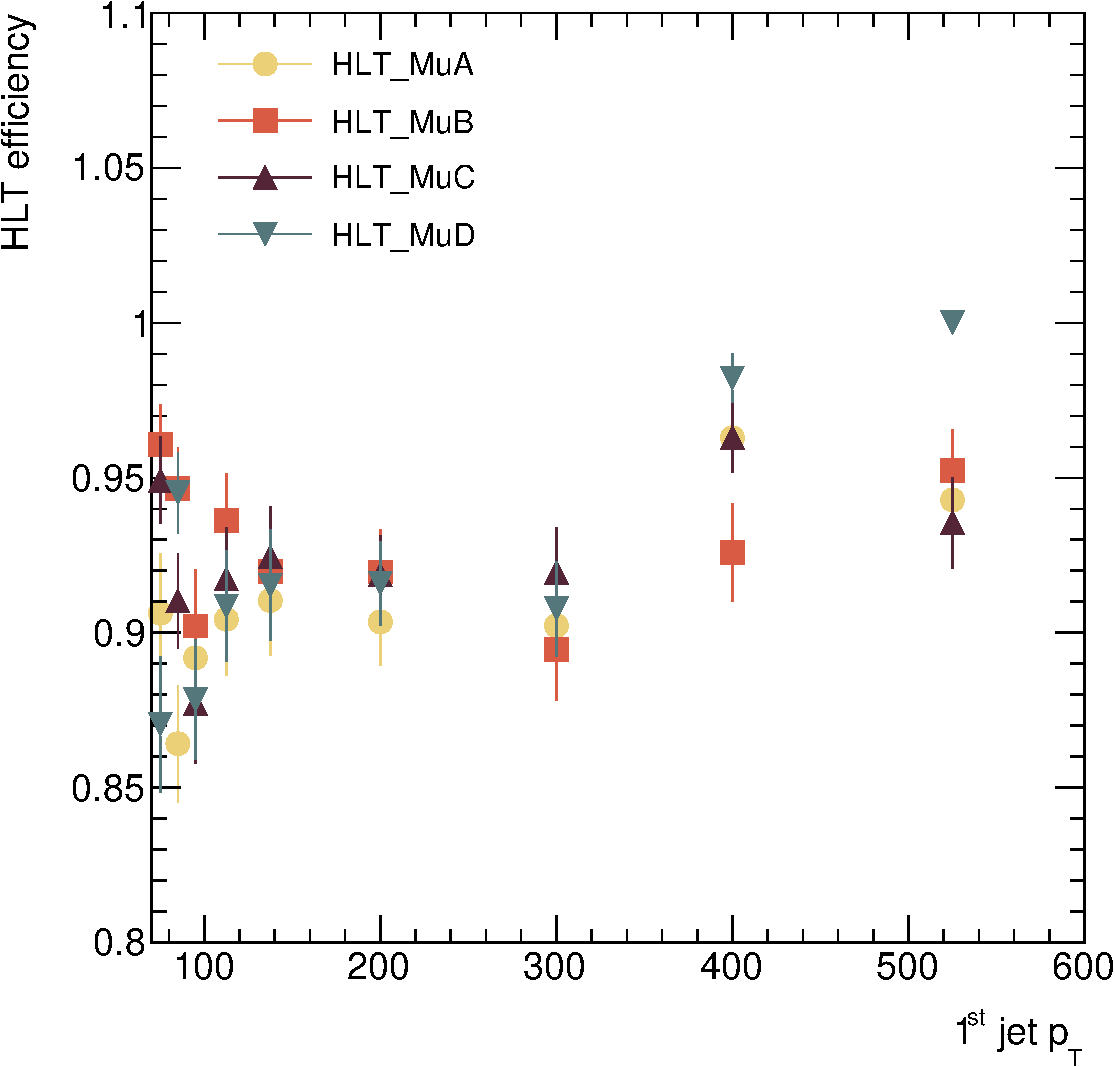
\includegraphics[width=0.48\textwidth]{chapitre7/figs/HLT/HLTturnon_mu_firstJet_zoom.pdf}} \hfill
%     \subcaptionbox{\ordinalnum{2} jet}[0.48\textwidth]{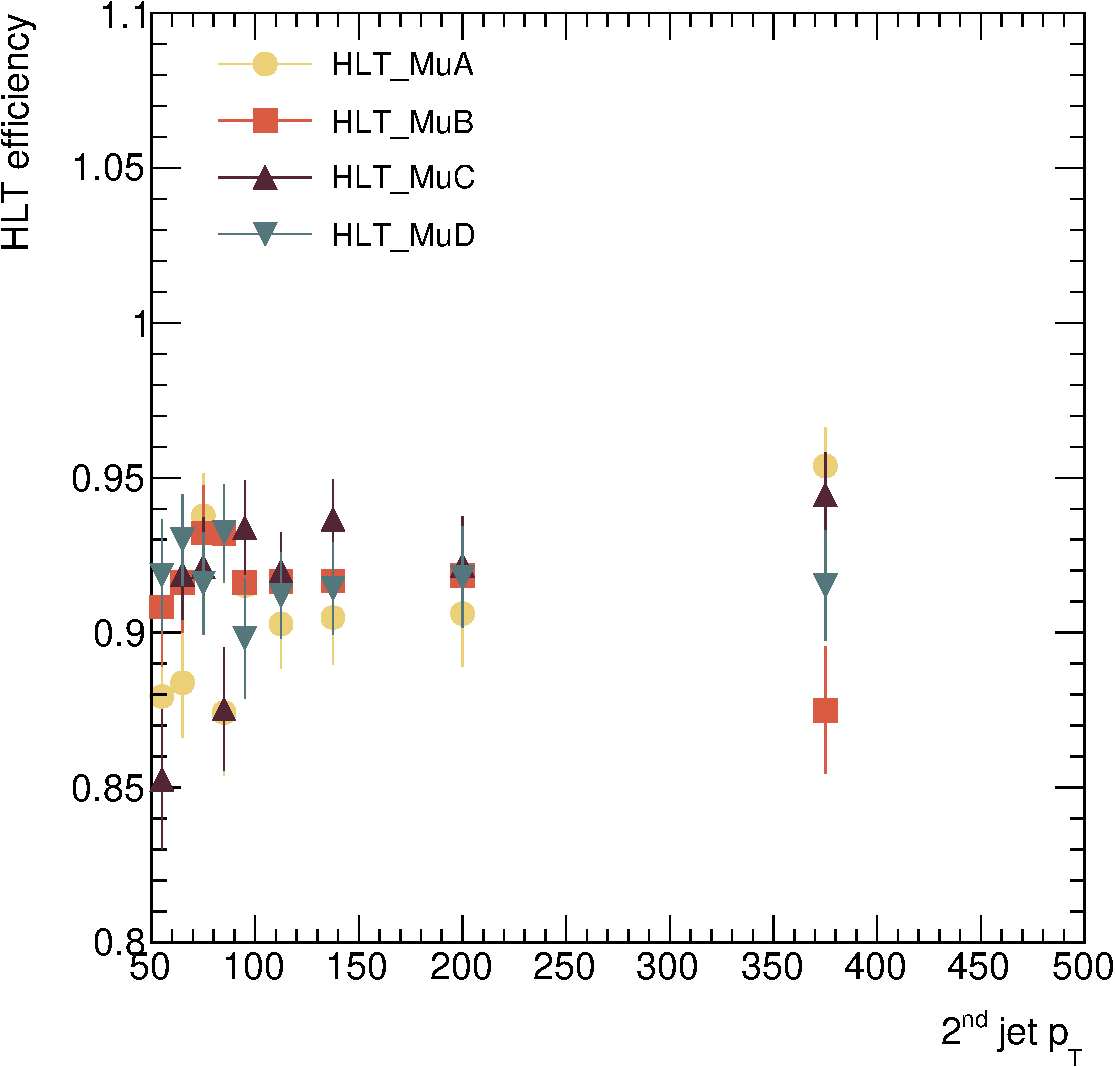
\includegraphics[width=0.48\textwidth]{chapitre7/figs/HLT/HLTturnon_mu_secondJet_zoom.pdf}} \\
%     \subcaptionbox{\ordinalnum{3} jet}[0.48\textwidth]{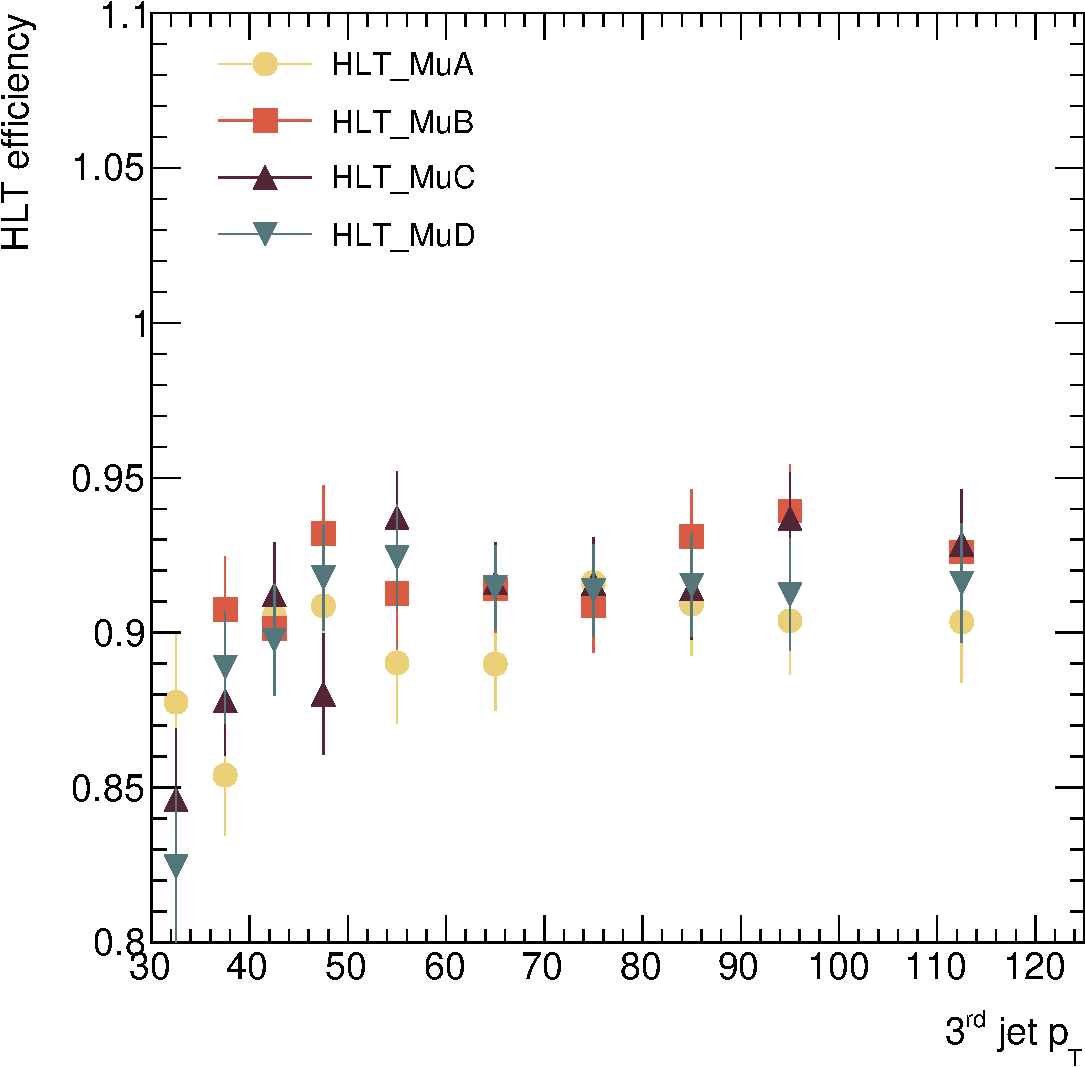
\includegraphics[width=0.48\textwidth]{chapitre7/figs/HLT/HLTturnon_mu_thirdJet_zoom.pdf}} \hfill
%     \subcaptionbox{\ordinalnum{4} jet}[0.48\textwidth]{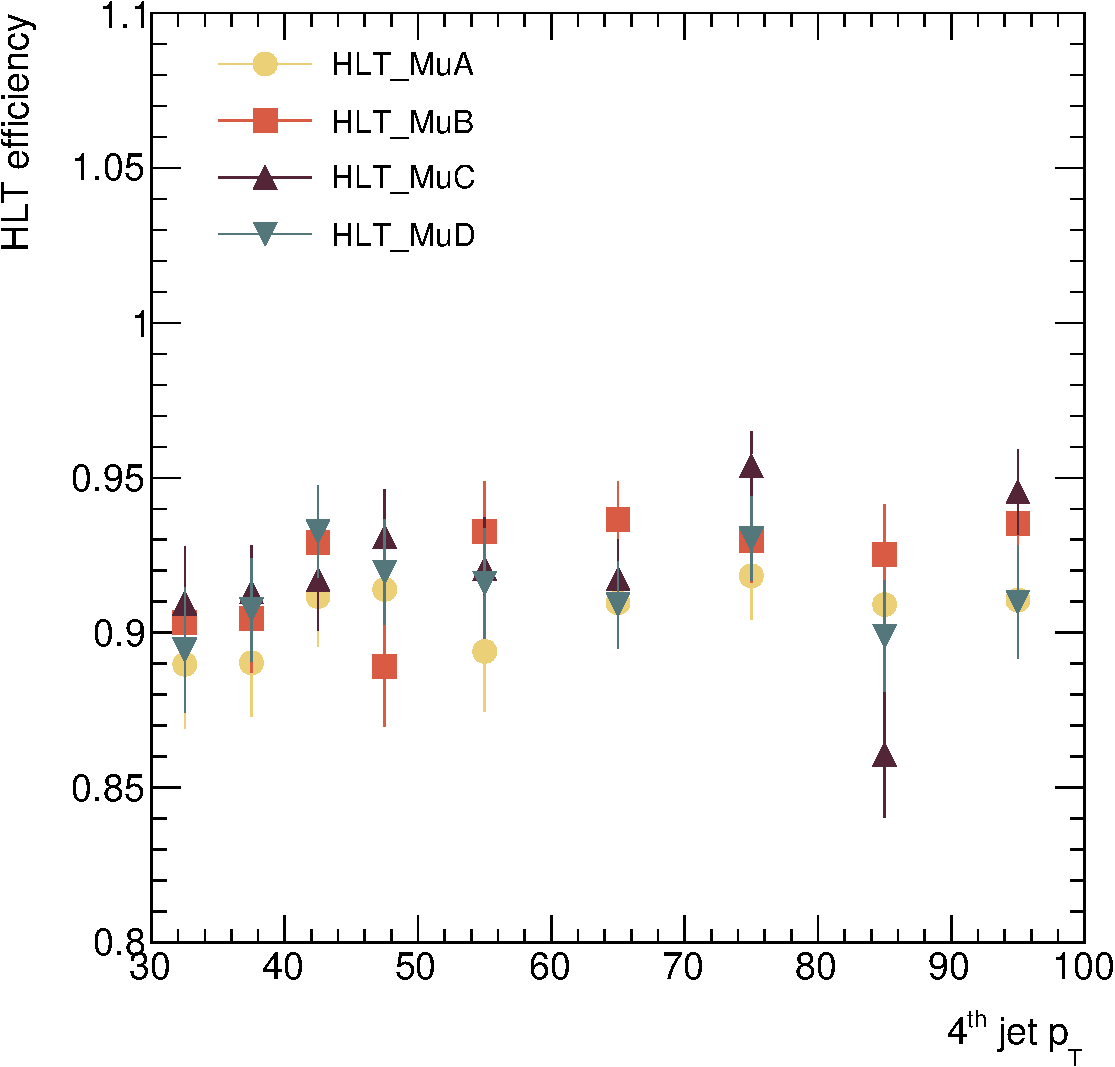
\includegraphics[width=0.48\textwidth]{chapitre7/figs/HLT/HLTturnon_mu_fourthJet_zoom.pdf}}
%     \caption{Efficacité des chemins de déclenchements en fonction de l'impulsion des quatre premiers jets de l'événement pour le canal semi-muonique.}
%     \label{fig:trig_eff_mu_jets}
% \end{figure}

% \begin{figure}[tbp] \centering
%     \subcaptionbox{\ordinalnum{1} jet}[0.48\textwidth]{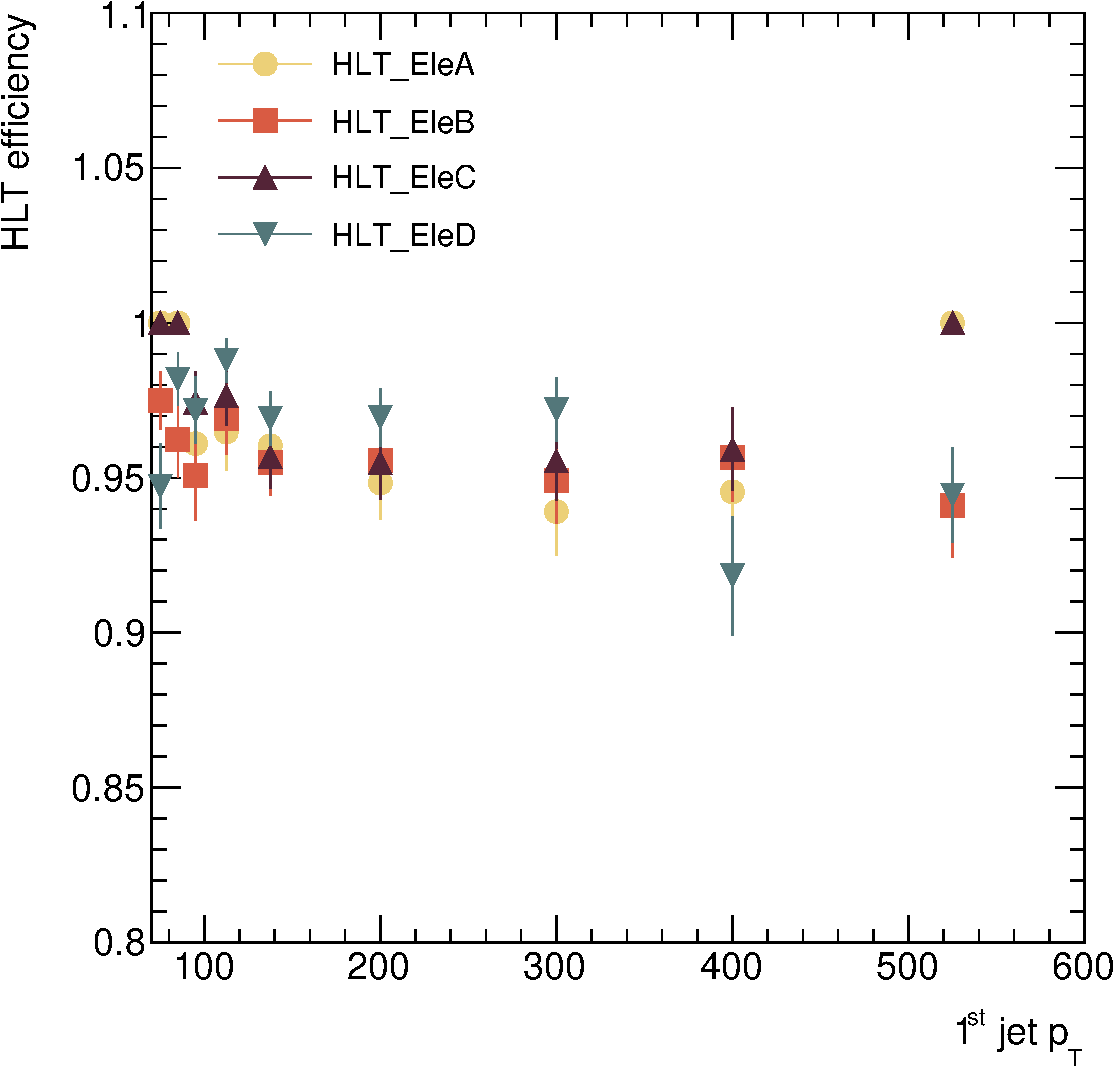
\includegraphics[width=0.48\textwidth]{chapitre7/figs/HLT/HLTturnon_el_firstJet_zoom.pdf}} \hfill
%     \subcaptionbox{\ordinalnum{2} jet}[0.48\textwidth]{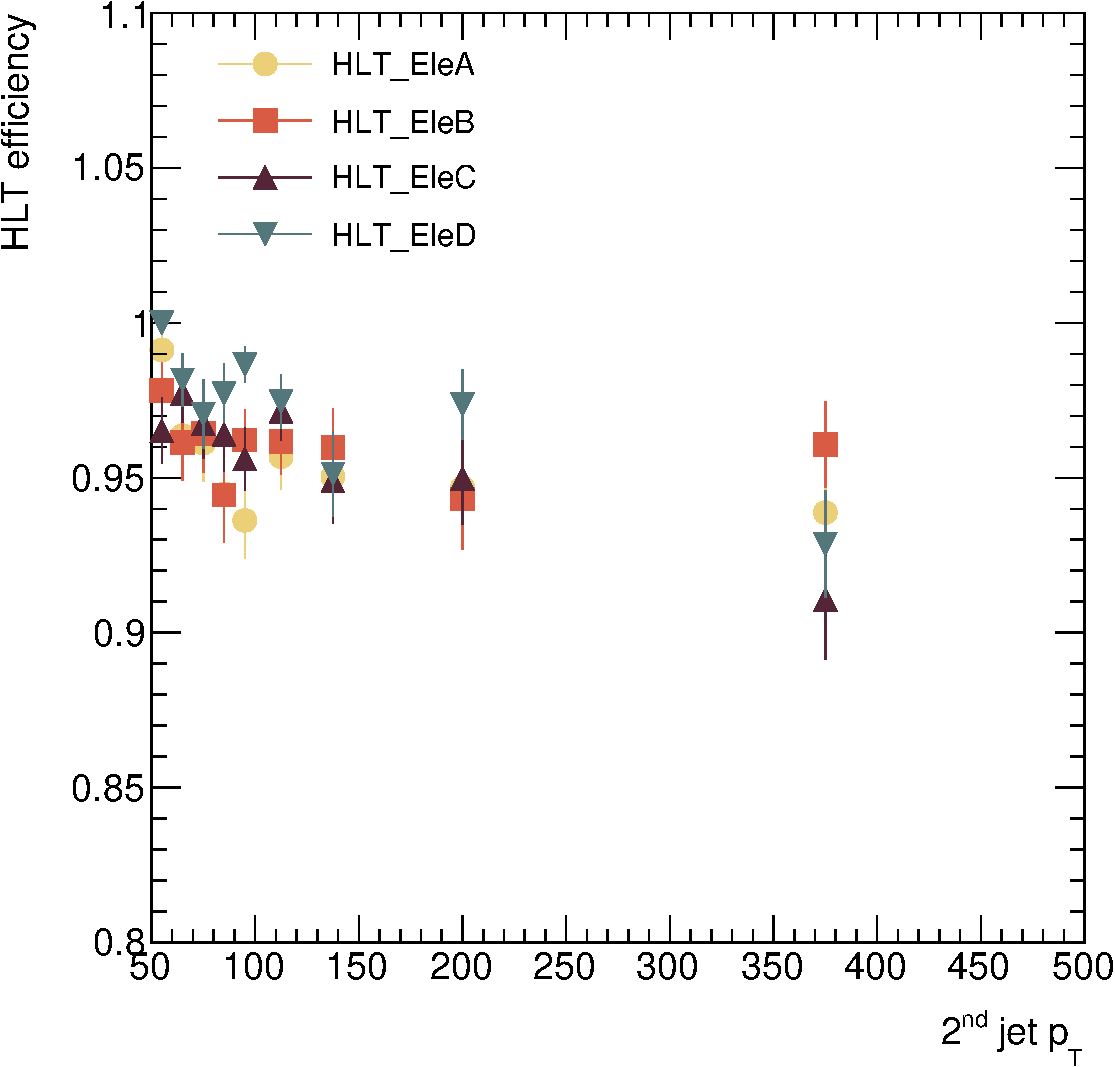
\includegraphics[width=0.48\textwidth]{chapitre7/figs/HLT/HLTturnon_el_secondJet_zoom.pdf}} \\
%     \subcaptionbox{\ordinalnum{3} jet}[0.48\textwidth]{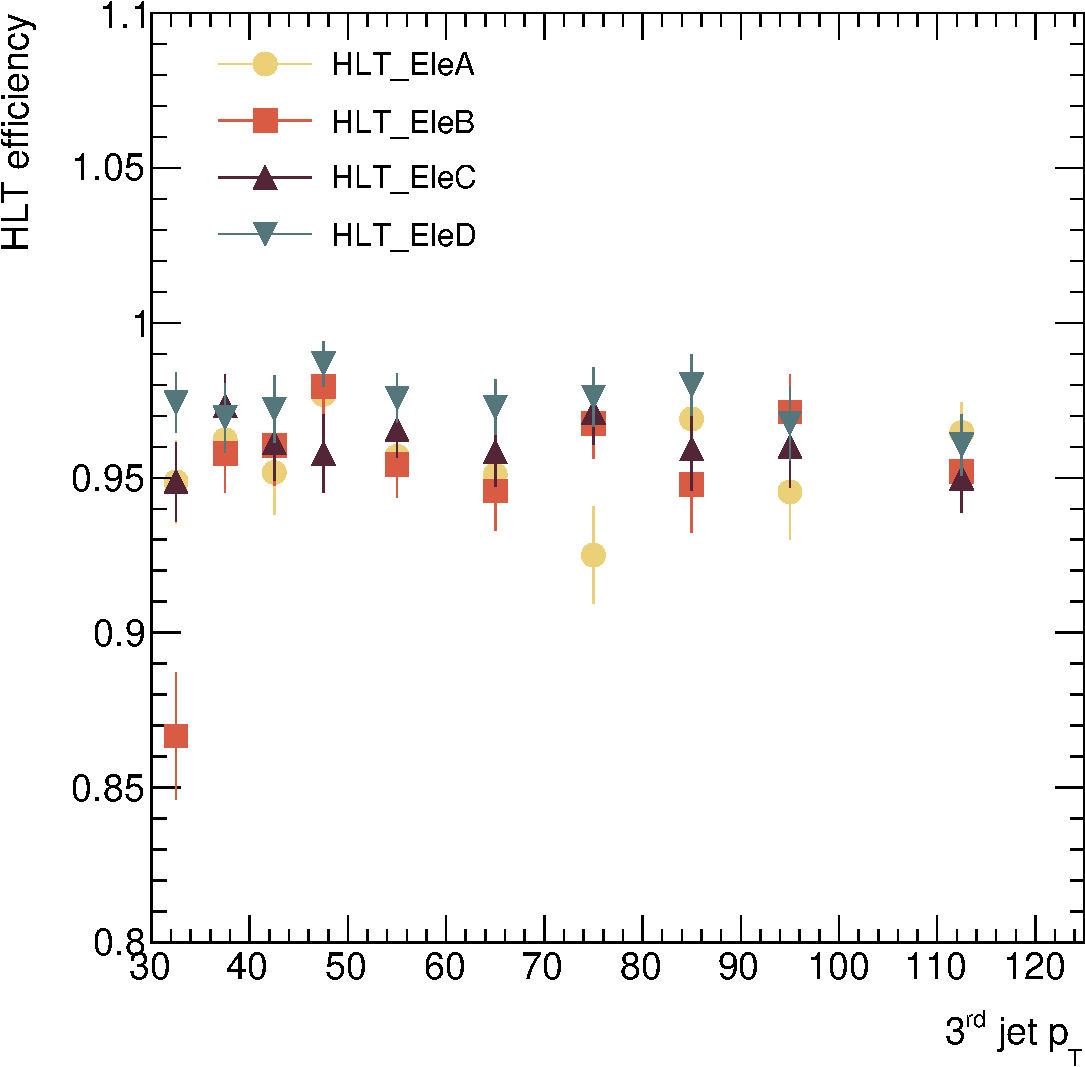
\includegraphics[width=0.48\textwidth]{chapitre7/figs/HLT/HLTturnon_el_thirdJet_zoom.pdf}} \hfill
%     \subcaptionbox{\ordinalnum{4} jet}[0.48\textwidth]{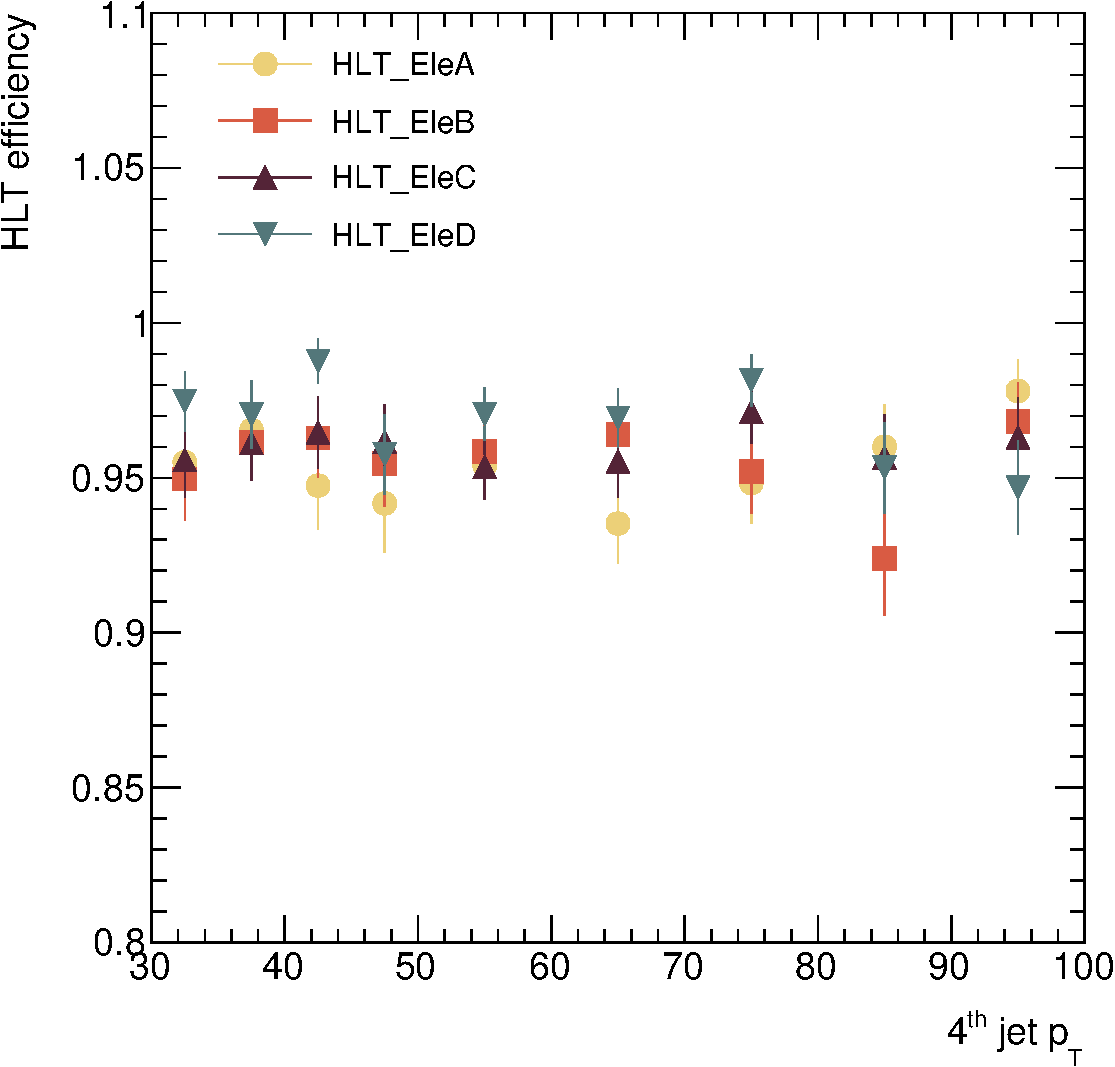
\includegraphics[width=0.48\textwidth]{chapitre7/figs/HLT/HLTturnon_el_fourthJet_zoom.pdf}}
%     \caption{Efficacité des chemins de déclenchements en fonction de l'impulsion des quatre premiers jets de l'événement pour le canal semi-électronique.}
%     \label{fig:trig_eff_e_jets}
% \end{figure}

\subsection{Efficacité de sélection} \label{sec:zprime_eff_sel}

\begin{table}[p!] \centering
  \begin{tabular}{ccccccc} \toprule
    & \SI{500}{\GeV} & \SI{750}{\GeV} & \SI{1000}{\GeV} & \SI{1250}{\GeV} & \SI{1500}{\GeV} & \SI{2000}{\GeV} \\ \midrule
    $\epsilon$, semi-$\mu$ & \num{0.55 \pm 0.02} & \num{1.60 \pm 0.03} & \num{1.87 \pm 0.03} & \num{1.86 \pm 0.03} & \num{1.63 \pm 0.03} & \num{1.13 \pm 0.02} \\
    $\epsilon$, semi-e & \num{0.47 \pm 0.01} & \num{1.43 \pm 0.03} & \num{1.74 \pm 0.03} & \num{1.80 \pm 0.03} & \num{1.61 \pm 0.03} & \num{1.22 \pm 0.03} \\ \bottomrule
  \end{tabular}
  \caption{Efficacités de sélection du signal pour différentes masses de \zprime dans l'hypothèse de résonances étroites, en demandant exactement 1 jet étiqueté \Pbottom. Ces efficacités sont calculés par rapport à la désintégration $\zprime \rightarrow \ttbar$ inclusive.}
  \label{tab:eff_narrow_1b}
\end{table}

\begin{table}[p!] \centering
  \begin{tabular}{ccccccc} \toprule
    & \SI{500}{\GeV} & \SI{750}{\GeV} & \SI{1000}{\GeV} & \SI{1250}{\GeV} & \SI{1500}{\GeV} & \SI{2000}{\GeV} \\ \midrule
    $\epsilon$, semi-$\mu$ & \num{0.51 \pm 0.01} & \num{1.62 \pm 0.03} & \num{1.90 \pm 0.03} & \num{1.67 \pm 0.03} & \num{1.38 \pm 0.03} & \num{0.81 \pm 0.02} \\
    $\epsilon$, semi-e & \num{0.43 \pm 0.01} & \num{1.46 \pm 0.03} & \num{1.68 \pm 0.03} & \num{1.57 \pm 0.03} & \num{1.32 \pm 0.03} & \num{0.81 \pm 0.02} \\ \bottomrule
  \end{tabular}
  \caption{Efficacités de sélection du signal pour différentes masses de \zprime dans l'hypothèse de résonances étroites, en demandant au moins 2 jets étiquetés \Pbottom. Ces efficacités sont calculés par rapport à la désintégration $\zprime \rightarrow \ttbar$ inclusive.}
  \label{tab:eff_narrow_2b}
\end{table}

\begin{table}[p!] \centering
  \begin{tabular}{ccccccc} \toprule
    & \SI{500}{\GeV} & \SI{750}{\GeV} & \SI{1000}{\GeV} & \SI{1250}{\GeV} & \SI{1500}{\GeV} & \SI{2000}{\GeV} \\ \midrule
    $\epsilon$, semi-$\mu$ & \num{0.66 \pm 0.02} & \num{1.57 \pm 0.03} & \num{1.89 \pm 0.03} & \num{1.81 \pm 0.03} & \num{1.65 \pm 0.03} & \num{1.31 \pm 0.03} \\
    $\epsilon$, semi-e & \num{0.48 \pm 0.02} & \num{1.25 \pm 0.02} & \num{1.63 \pm 0.03} & \num{1.60 \pm 0.03} & \num{1.66 \pm 0.03} & \num{1.28 \pm 0.03} \\ \bottomrule
  \end{tabular}
  \caption{Efficacités de sélection du signal pour différentes masses de \zprime dans l'hypothèse de résonances larges, en demandant exactement 1 jet étiqueté \Pbottom. Ces efficacités sont calculés par rapport à la désintégration $\zprime \rightarrow \ttbar$ inclusive.}
  \label{tab:eff_large_1b}
\end{table}

\begin{table}[p!] \centering
  \begin{tabular}{ccccccc} \toprule
    & \SI{500}{\GeV} & \SI{750}{\GeV} & \SI{1000}{\GeV} & \SI{1250}{\GeV} & \SI{1500}{\GeV} & \SI{2000}{\GeV} \\ \midrule
    $\epsilon$, semi-$\mu$ & \num{0.62 \pm 0.02} & \num{1.60 \pm 0.03} & \num{1.81 \pm 0.03} & \num{1.64 \pm 0.03} & \num{1.40 \pm 0.03} & \num{1.07 \pm 0.02} \\
    $\epsilon$, semi-e & \num{0.48 \pm 0.02} & \num{1.38 \pm 0.03} & \num{1.55 \pm 0.03} & \num{1.52 \pm 0.04} & \num{1.35 \pm 0.04} & \num{1.02 \pm 0.02} \\ \bottomrule
  \end{tabular}
  \caption{Efficacités de sélection du signal pour différentes masses de \zprime dans l'hypothèse de résonances larges, en demandant au moins 2 jets étiquetés \Pbottom. Ces efficacités sont calculés par rapport à la désintégration $\zprime \rightarrow \ttbar$ inclusive.}
  \label{tab:eff_large_2b}
\end{table}

\begin{table}[p!] \centering
  \begin{tabular}{ccccccc} \toprule
    & \SI{500}{\GeV} & \SI{700}{\GeV} & \SI{1000}{\GeV} & \SI{1200}{\GeV} & \SI{1500}{\GeV} \\ \midrule
    $\epsilon$, semi-$\mu$ & \num{1.26 \pm 0.04} & \num{1.55 \pm 0.04} & \num{1.53 \pm 0.03} & \num{1.48 \pm 0.04} & \num{1.20 \pm 0.03} \\
    $\epsilon$, semi-e & \num{1.09 \pm 0.03} & \num{1.36 \pm 0.04} & \num{1.50 \pm 0.03} & \num{1.33 \pm 0.04} & \num{1.25 \pm 0.04} \\ \bottomrule
  \end{tabular}
  \caption{Efficacités de sélection du signal pour différentes masses de \kkglu, en demandant exactement 1 jet étiqueté \Pbottom. Ces efficacités sont calculés par rapport à la désintégration $\kkg \rightarrow \ttbar$ inclusive.}
  \label{tab:eff_kk_1b}
\end{table}

\begin{table}[tbp] \centering
  \begin{tabular}{ccccccc} \toprule
    & \SI{500}{\GeV} & \SI{700}{\GeV} & \SI{1000}{\GeV} & \SI{1200}{\GeV} & \SI{1500}{\GeV} \\ \midrule
    $\epsilon$, semi-$\mu$ & \num{1.25 \pm 0.04} & \num{1.47 \pm 0.04} & \num{1.40 \pm 0.03} & \num{1.26 \pm 0.04} & \num{1.02 \pm 0.03} \\
    $\epsilon$, semi-e & \num{1.08 \pm 0.03} & \num{1.38 \pm 0.04} & \num{1.35 \pm 0.03} & \num{1.27 \pm 0.04} & \num{0.96 \pm 0.03} \\ \bottomrule
  \end{tabular}
  \caption{Efficacités de sélection du signal pour différentes masses de \kkglu, en demandant au moins 2 jets étiquetés \Pbottom. Ces efficacités sont calculés par rapport à la désintégration $\kkg \rightarrow \ttbar$ inclusive.}
  \label{tab:eff_kk_2b}
\end{table}

Les \cref{tab:eff_narrow_1b,tab:eff_narrow_2b} présentent les efficacités de sélection pour différentes masses de \zprime dans l'hypothèse de résonances étroites et pour les 4 catégories de l'analyse. Ces efficacités sont inclusives, c'est-à-dire calculées en considérant tous les canaux de désintégrations des paires \ttbar, et pas seulement le canal semi-leptonique. De façon équivalente, les efficacités obtenues dans le cas de \zprime larges sont résumées dans les \cref{tab:eff_large_1b,tab:eff_large_2b}, et dans les \cref{tab:eff_kk_1b,tab:eff_kk_2b} dans le cas des gluons de Kaluza-Klein. Toutes ces efficacités sont calculées après avoir appliqué une coupure supplémentaire $\mtt > \SI{550}{\GeV}$ (les raisons d'un tel choix sont décrites plus loin dans ce chapitre). Cette coupure explique pourquoi l'efficacité de sélection pour la résonance à \SI{500}{\GeV} est faible comparée aux autres masses.

\bigskip

Afin d'obtenir l'efficacité de sélection d'un éventuel signal sur les données, des facteurs de correction sont appliqués pour tenir compte des différences de performances de l'algorithme d'étiquetage des \Pbottom ainsi que l'efficacité d'identification et d'isolation des leptons entre la simulation et les données. Ces facteurs de corrections sont disponibles pour toutes les analyses, et dépendent de l'impulsion transverse et de la pseudo-rapidité des objets physiques concernés. Pour obtenir un facteur de correction global à appliquer aux efficacités de sélection, les valeurs centrales sont combinées en tenant compte des spectres en \pt et \aeta des objets physique du signal. On obtient au final les facteurs de corrections suivants, définis par le rapport $\epsilon_{\text{données}} \, / \, \epsilon_{\text{MC}}$ :
\begin{itemize}
  \item Identification et isolation des muons : \num{0.992 \pm 0.005}.
  \item Identification et isolation des électrons : \num{0.982 \pm 0.003}.
  \item Étiquetage des jets de \Pbottom : \num{1.043 \pm 0.022} pour exactement 1 jet étiqueté \Pbottom, et \num{0.927 \pm 0.038} pour au moins deux jets étiquetés \Pbottom.
\end{itemize}

\section{Stratégie de l'analyse}

Pour détecter d'éventuelles résonances dans le spectre de masse invariante de paires \ttbar, on reconstruit dans un premier temps \mtt à l'aide des méthodes présentées dans le \cref{chap:mtt_reco}. Plus précisément, on utilise l'algorithme de tri par $\chi^2$ pour sélectionner la bonne combinaison de jets. Les performances de cet algorithme sur des événements \zprime sont détaillées plus loin.

\smallskip

Il faut ensuite être capable de comparer le spectre \mtt reconstruit à l'aide des données collectées aux prédictions théoriques du Modèle Standard. Une première méthode consiste à estimer chacun ou une partie des bruits de fond en utilisant la simulation. Cette méthode nécessite d'avoir une excellente connaissance des générateurs d'événements, et introduit de nombreuses sources d'erreurs systématiques. Afin de réduire ces erreurs, il est possible d'estimer le bruit de fond directement sur les données, en utilisant une interpolation et la connaissance de la forme des distributions. On s'affranchit ainsi de toutes les incertitudes liées à l'utilisation de la simulation pour modéliser les bruits de fond. C'est cette méthode qui est utilisée dans l'analyse, la simulation étant utilisée uniquement pour obtenir la forme du signal, ainsi que l'efficacité de sélection. On sélectionne uniquement la région $\mtt > \SI{550}{\GeV}$ afin de n'avoir qu'un fond strictement décroissant.

\smallskip

Une fois les bruits de fond estimés, la confrontation entre données et prédictions est possible. Toute déviation par rapport au bruit de fond attendu peut être due à la présence de signal, ou à une simple fluctuation statistique. Une analyse statistique est réalisée afin d'évaluer la signification statistique d'un éventuel signal, et, en cas d'absence de signal, de poser des limites sur les sections efficaces de production des processus de nouvelle physique. Cette procédure sera détaillée dans la \cref{sec:stat}.

%Si les deux sont en accord, cela ne veut pas forcément dire qu'un signal n'est présent, mais seulement que l'analyse n'est pas (encore) sensible à ce type de signal, à cause de mauvaises performances de reconstruction ou des sections efficaces théoriques trop faible face à la luminosité collectée. On utilise alors une méthode statistique afin de mettre des limites sur les sections efficaces des processus de nouvelle physique. Cette procédure sera détaillée dans la \cref{sec:stat}.

\subsection{Performances de la reconstruction pour le signal}

\begin{figure}[tbp]
  \centering
  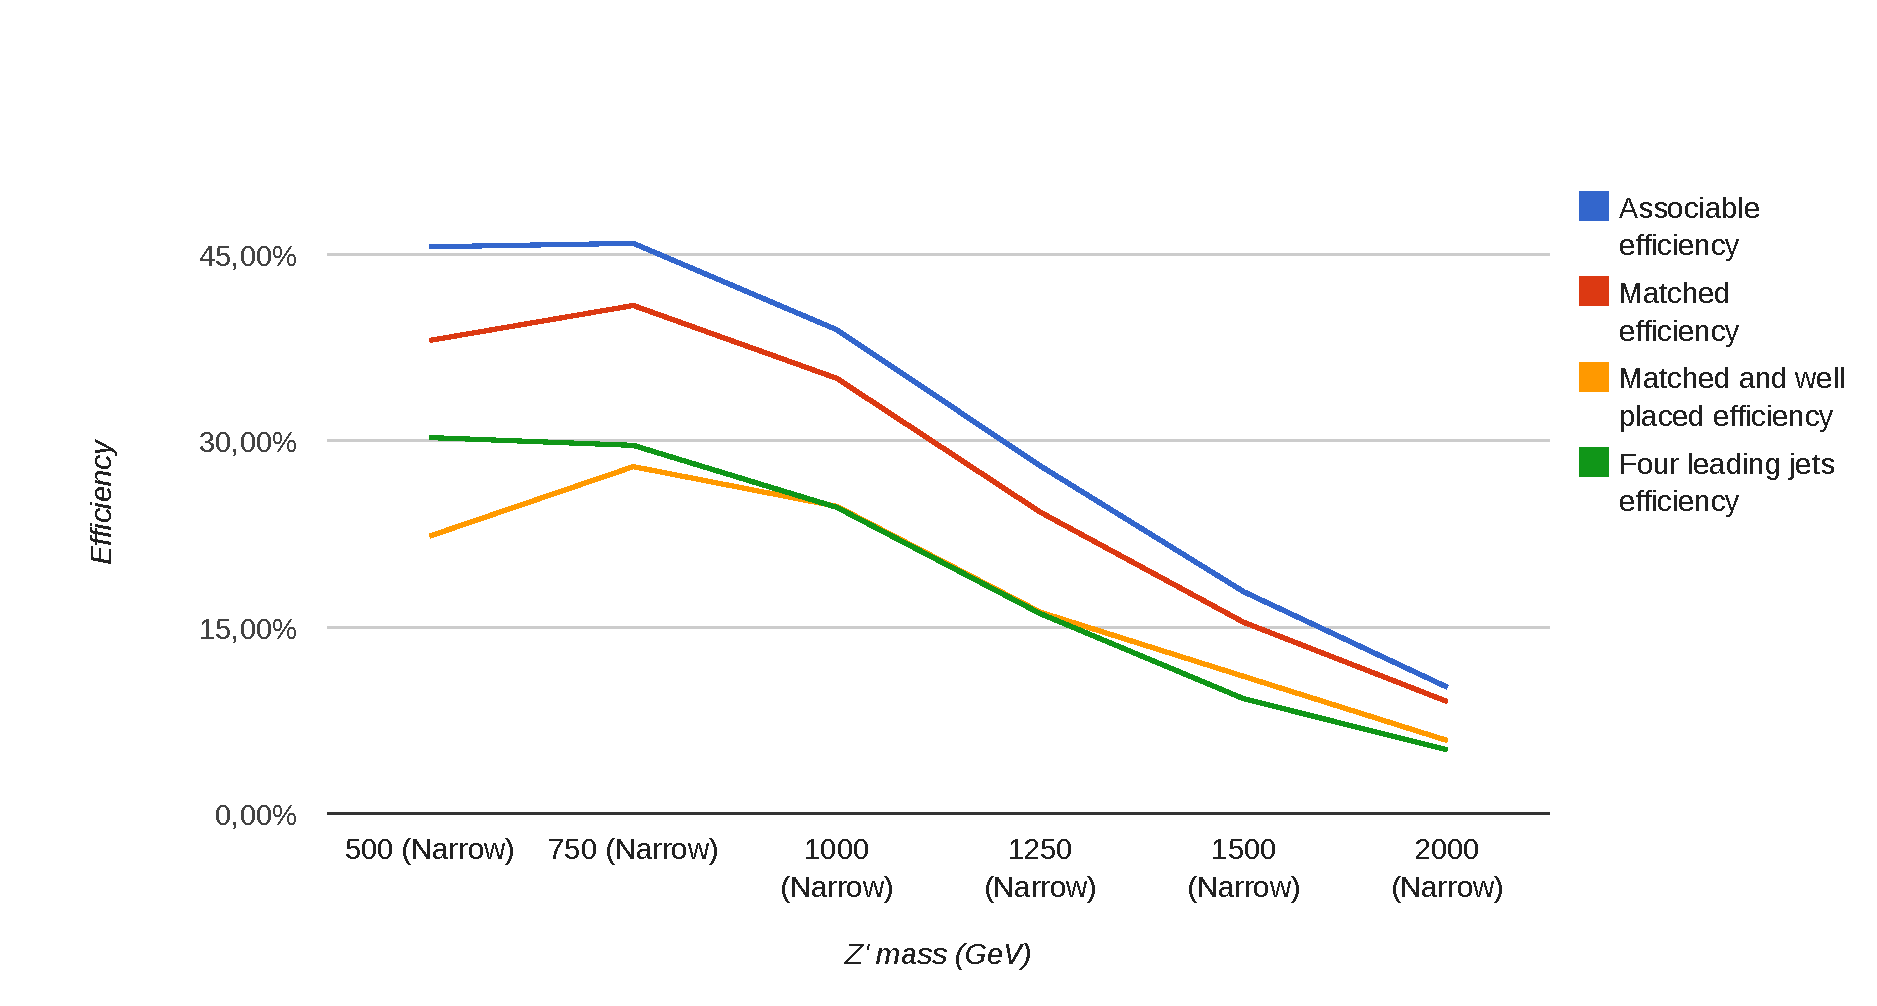
\includegraphics[width=0.9\textwidth]{chapitre7/figs/chi2_eff_vs_zprime_mass.pdf}
  \caption{Évolution de l'efficacité d'avoir un événement associable (bleu), un événement associé (rouge), et un événement associé et bien placé (jaune) en fonction de la masse des résonances, dans l'hypothèse de résonances étroites. A titre de comparaison, l'efficacité de choisir la bonne combinaison de jets en utilisant les 4 premiers jets de l'événement est présentée en vert. Les efficacités présentées sont absolues, c'est-à-dire par exemple $\epsilon^\prime_\text{associé} \equiv \epsilon_\text{associable} \times \epsilon_\text{associé}$.}
  \label{fig:eff_vs_zprime}
\end{figure}

Les performances de l'algorithme de $\chi^2$ ont été présentées dans la \cref{sec:perf_reco_tt} pour des événements \ttbar Modèle Standard. Cette section est dédiée aux performances de cet algorithme sur des événements \ttbar provenant de la désintégration d'un \zprime.

La \cref{fig:eff_vs_zprime} présente l'évolution des efficacités liées à l'algorithme de $\chi^2$ (voir \cpageref{page:chi2_def} pour les définitions) en fonction de la masse des résonances. Pour des résonances légères (\num{500} et \SI{750}{\GeV}), l'efficacité d'avoir un événement associé est légèrement supérieure à celle du Modèle Standard (\tilde\SI{45}{\%} contre \tilde\SI{40}{\%}). Cependant, dès qu'on franchit le seuil du \si{\TeV}, cette efficacité chute fortement jusqu'à descendre sous les \SI{15}{\%} à \SI{2}{\TeV}. Cette baisse d'efficacité s'explique par la sélection employée par l'analyse. En demandant au moins 4 jets et un lepton isolé, l'analyse est optimisée pour les topologies non-boostées, c'est-à-dire où il est possible d'identifier chaque produit issu de la désintégration du système \ttbar. À partir du \si{\TeV}, les désintégrations deviennent boostées, ce qui peut avoir plusieurs conséquences :
\begin{itemize}
  \item Le lepton n'est plus nécessairement isolé.
  \item Étant boostés, les jets provenant de la désintégration du boson \PW hadronique voire du quark top hadronique peuvent se retrouver agglomérés au sein d'un même jet. L'événement comporte alors seulement 3 (2) jets provenant de la désintégration du système \ttbar, et non 4.
\end{itemize}
Afin de contourner ce problème, une autre analyse dédiée spécifiquement aux topologies boostées a été mise en place par une autre équipe. On verra à la fin de ce chapitre comment les résultats de notre analyse sont combinés avec cette analyse dédiée.

\medskip

\begin{figure}[tbp] \centering
    \subcaptionbox{$\mzp = \SI{750}{\GeV}$, résonance étroite.}[0.48\textwidth]{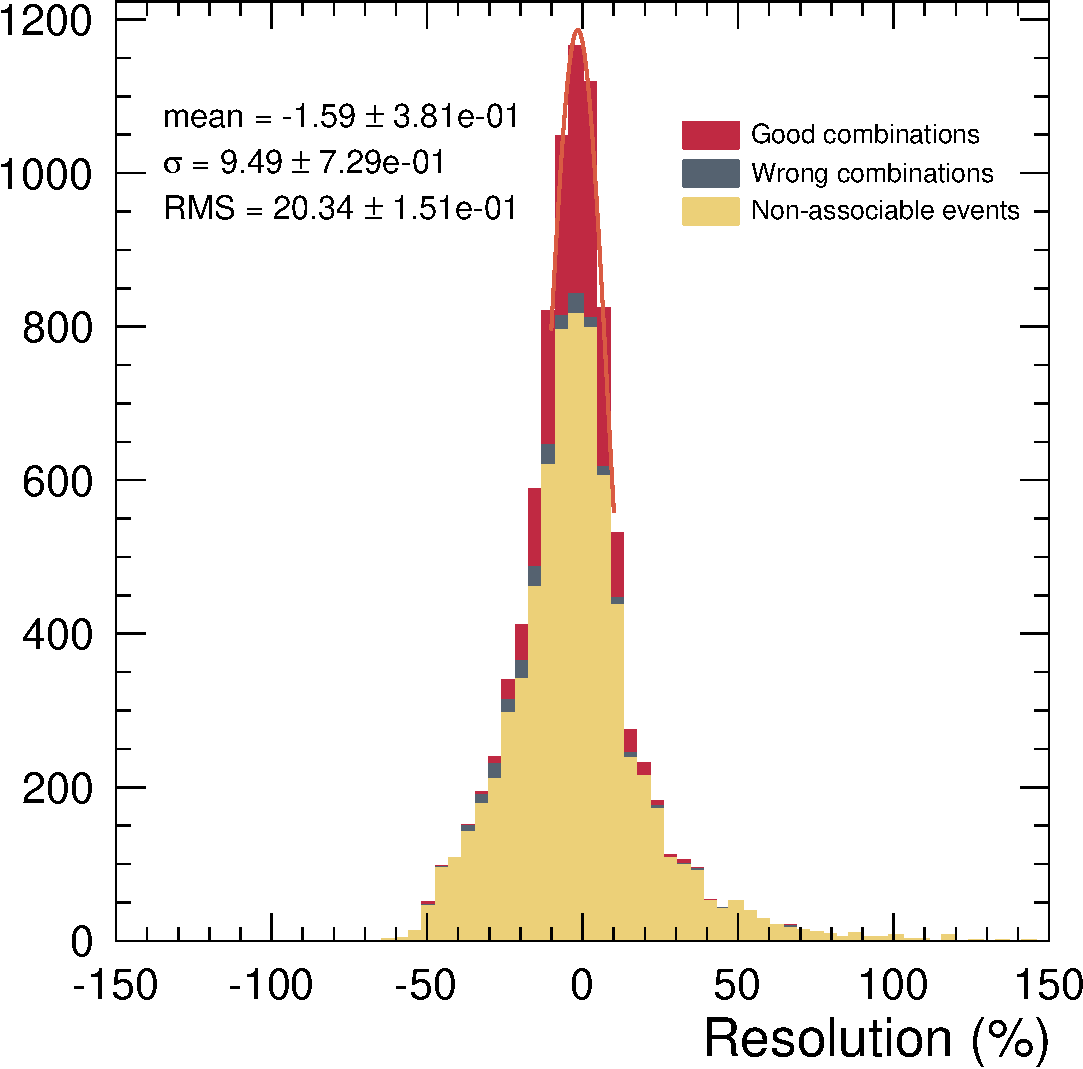
\includegraphics[width=0.48\textwidth]{chapitre7/figs/mtt_resolution_zprime_750_narrow.pdf}} \hfill
    \subcaptionbox{$\mzp = \SI{2000}{\GeV}$, résonance étroite.}[0.48\textwidth]{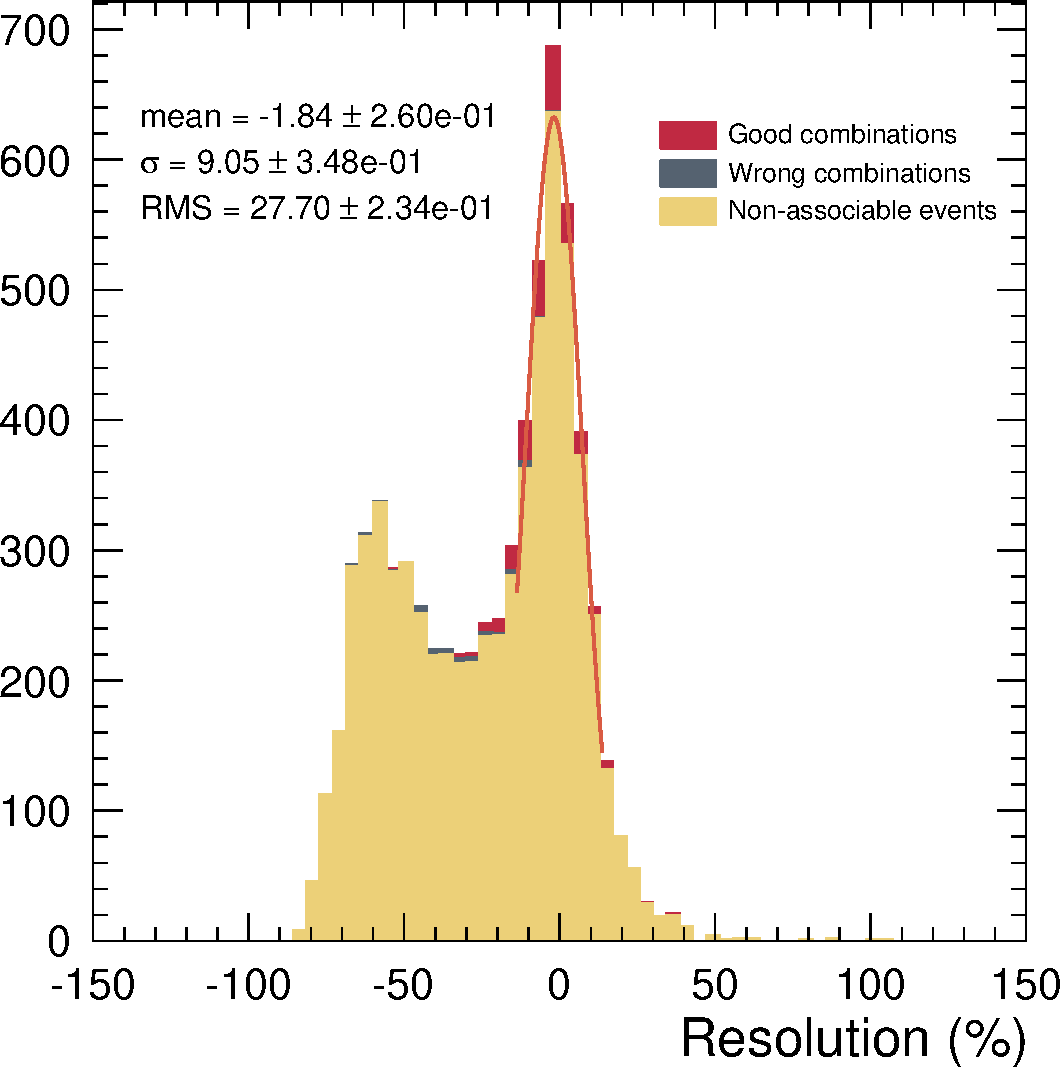
\includegraphics[width=0.48\textwidth]{chapitre7/figs/mtt_resolution_zprime_2000_narrow.pdf}}
    \caption{Résolution sur \mtt pour différentes masses de signal, représentée sous la forme d'un histogramme empilé. Les événements non-associables sont en jaune, ceux où la bonne combinaison de jets a été choisie en \rouge, et ceux où la mauvaise combinaison a été choisie en \gris.}
    \label{fig:mtt_reso_zprime}
\end{figure}

\begin{figure}[tbp] \centering
    \subcaptionbox{\label{fig:rms_zprime}}[0.48\textwidth]{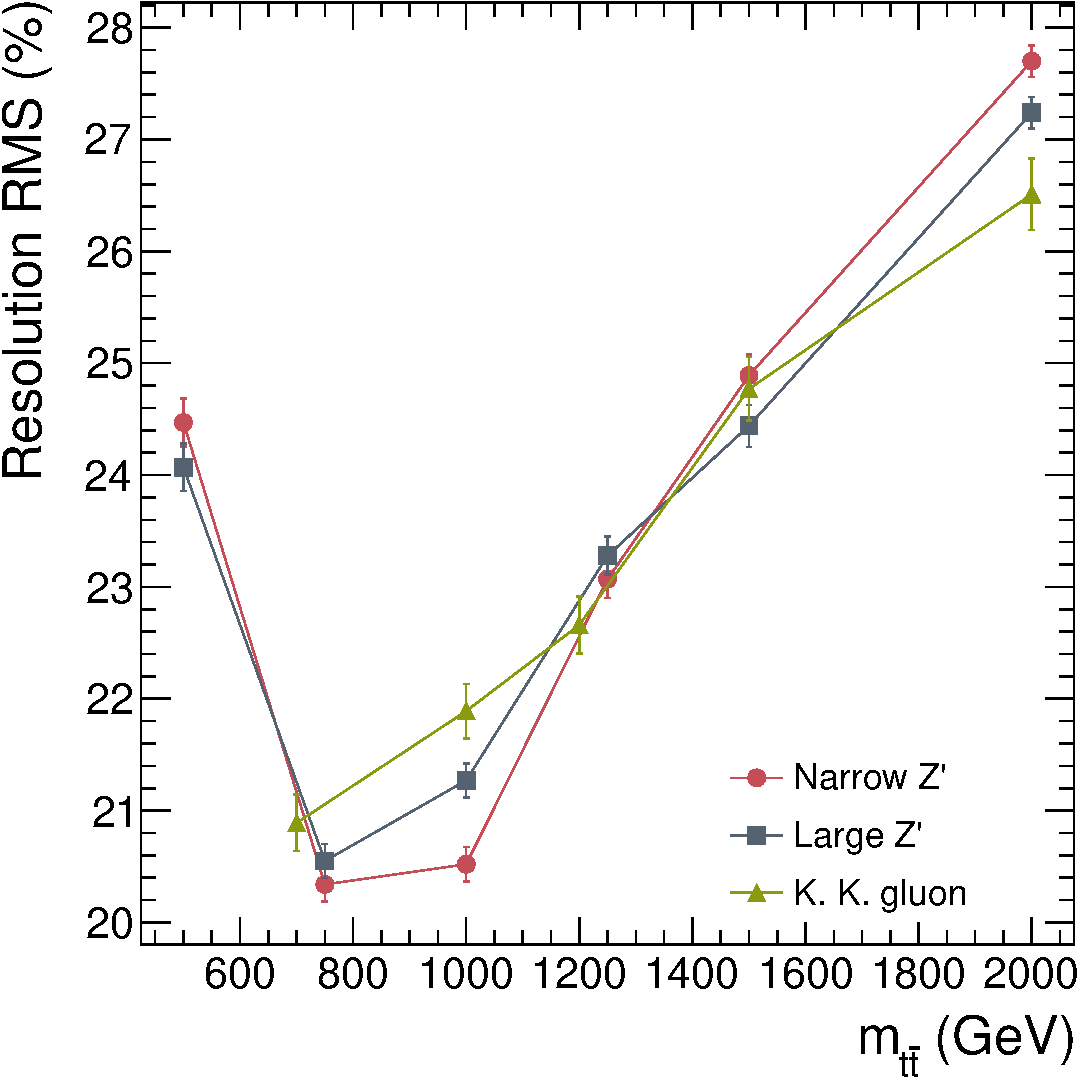
\includegraphics[width=0.48\textwidth]{chapitre7/figs/signal_rms_vs_mtt.pdf}} \hfill
    \subcaptionbox{\label{fig:reso_zprime}}[0.48\textwidth]{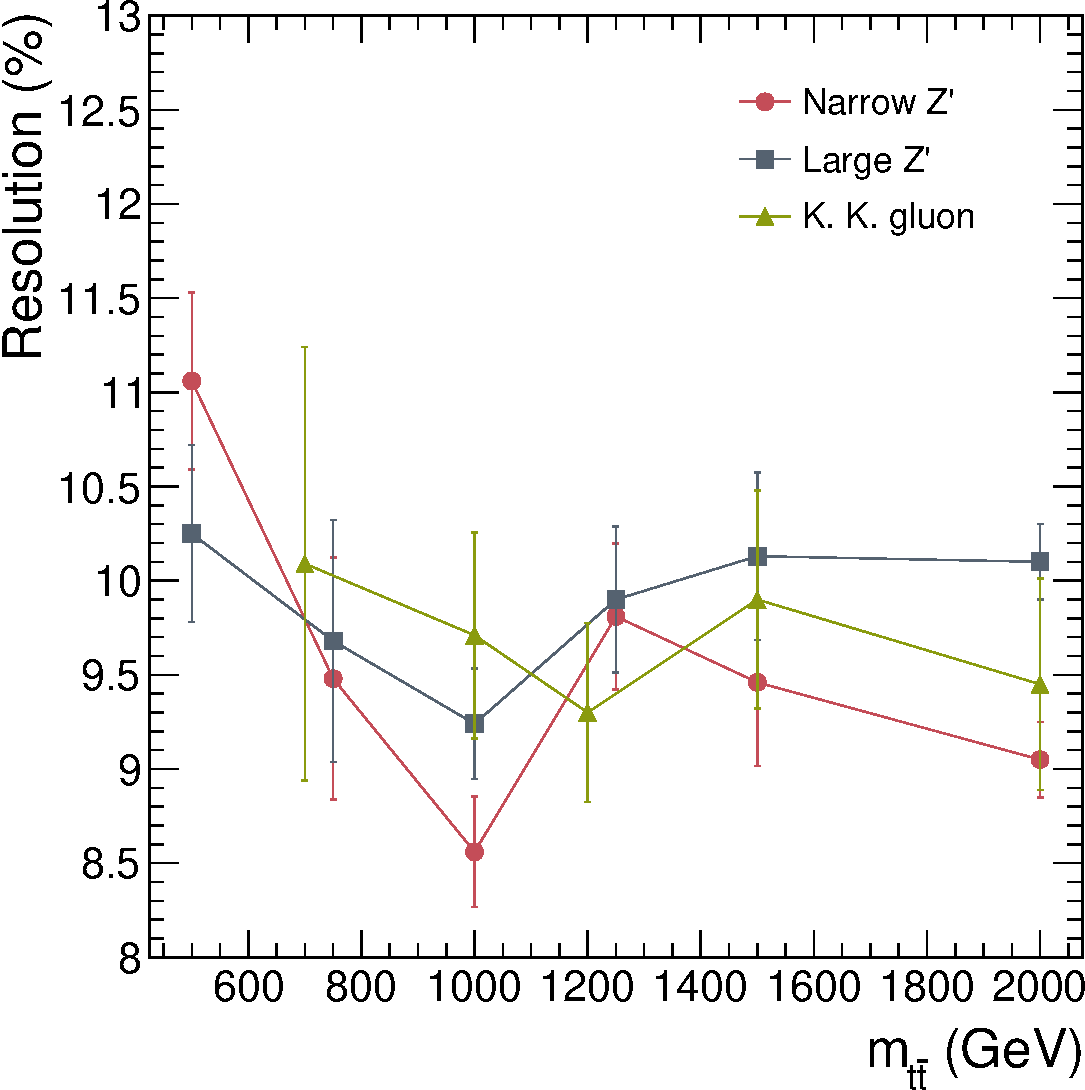
\includegraphics[width=0.48\textwidth]{chapitre7/figs/signal_reso_vs_mtt.pdf}}
    \caption{Évolution de la moyenne quadratique de la résolution (RMS) (\subref{fig:rms_zprime}) et de la résolution relative (\subref{fig:reso_zprime}), extraite à l'aide d'une interpolation gaussienne, en fonction de la masse de la résonance, pour chaque type de signal considéré.}
    \label{fig:rms_reso_zprime}
\end{figure}

Parmi les événements associables, l'efficacité de l'algorithme de $\chi^2$ reste stable en fonction de la masse de la résonance, augmentant même légèrement à haute masse, et reste supérieure à l'efficacité obtenue en choisissant uniquement les 4 jets de plus haut \pt. La \cref{fig:mtt_reso_zprime} présente les résolutions obtenues sur la masse invariante pour deux masses de résonances, dans l'hypothèse de résonances étroites. On constate l'apparition d'une distorsion de la résolution à haute masse, causée intégralement par les événements non-associables ou non-associés. Pour ces événements, on tente de reconstruire la masse invariante du système \ttbar en utilisant des jets ne provenant probablement pas de la désintégration du système \ttbar. D'ailleurs, en regardant l'évolution de la moyenne quadratique (RMS) de la résolution en fonction de la masse des résonances (\cref{fig:rms_zprime}), on constate que tous les modèles considérés se comportent de la même façon lorsque la masse de résonance augmente : une distorsion de la résolution apparaît, de plus en plus marquée à mesure que la masse augmente. Notons que la RMS est utilisée plutôt que la résolution relative extraite de l'interpolation gaussienne afin de quantifier la distorsion de la résolution à haute masse. La \cref{fig:reso_zprime} montre quant à elle l'évolution de la résolution, extraite à l'aide d'une interpolation gaussienne, en fonction de la masse de la résonance. On remarque ici que la résolution est quasiment identique pour chaque point de masse et pour chaque type de modèle. Face à cette dégradation de la résolution à haute masse, on s'attend d'ores et déjà à de mauvaises performances de l'analyse dans ces régions de signal.

\begin{figure}[tbp] \centering
    \subcaptionbox{\label{fig:kf_zp_750}}[0.48\textwidth]{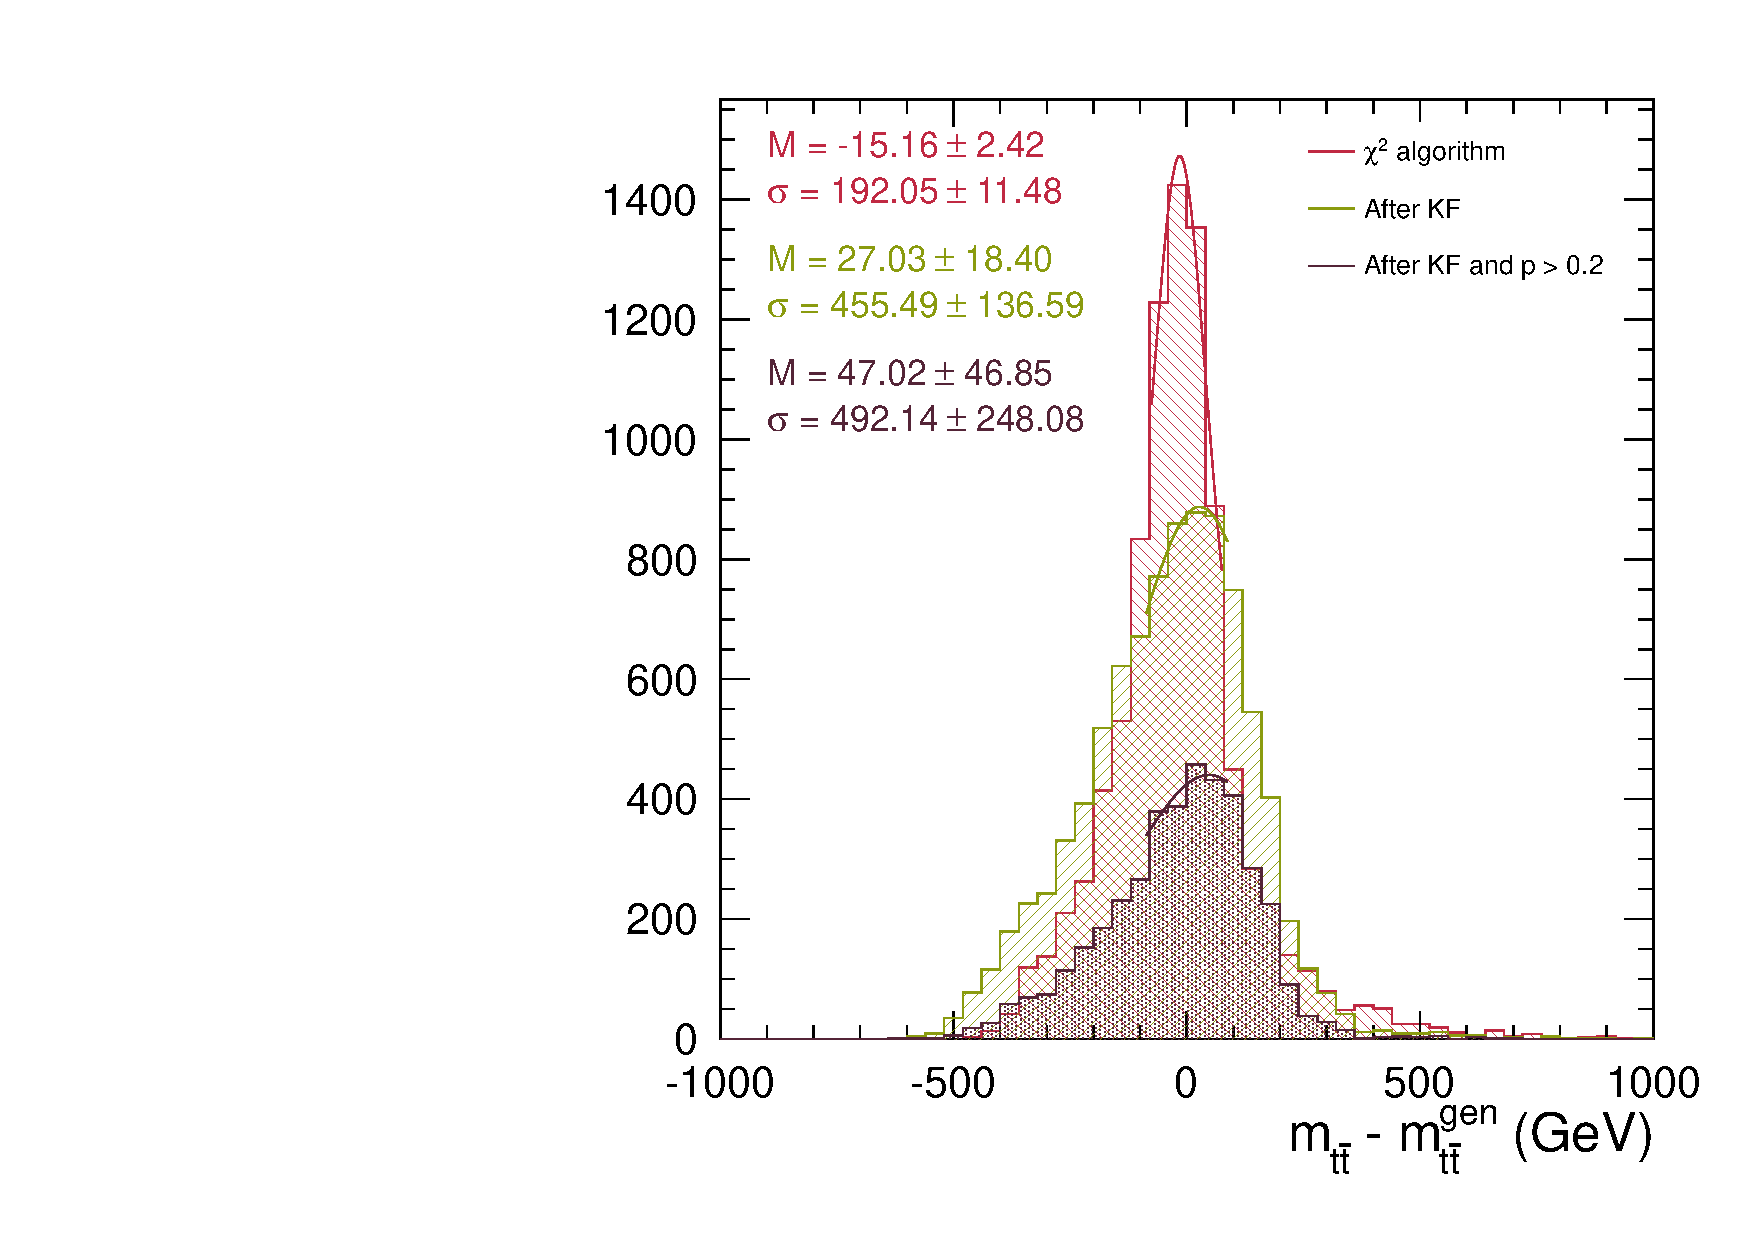
\includegraphics[width=0.48\textwidth,angle=-90,origin=c]{chapitre7/figs/kinfit/mtt_resolution_comparison_kf_zp750_all_events.pdf}} \hfill
    \subcaptionbox{\label{fig:kf_zp_2000}}[0.48\textwidth]{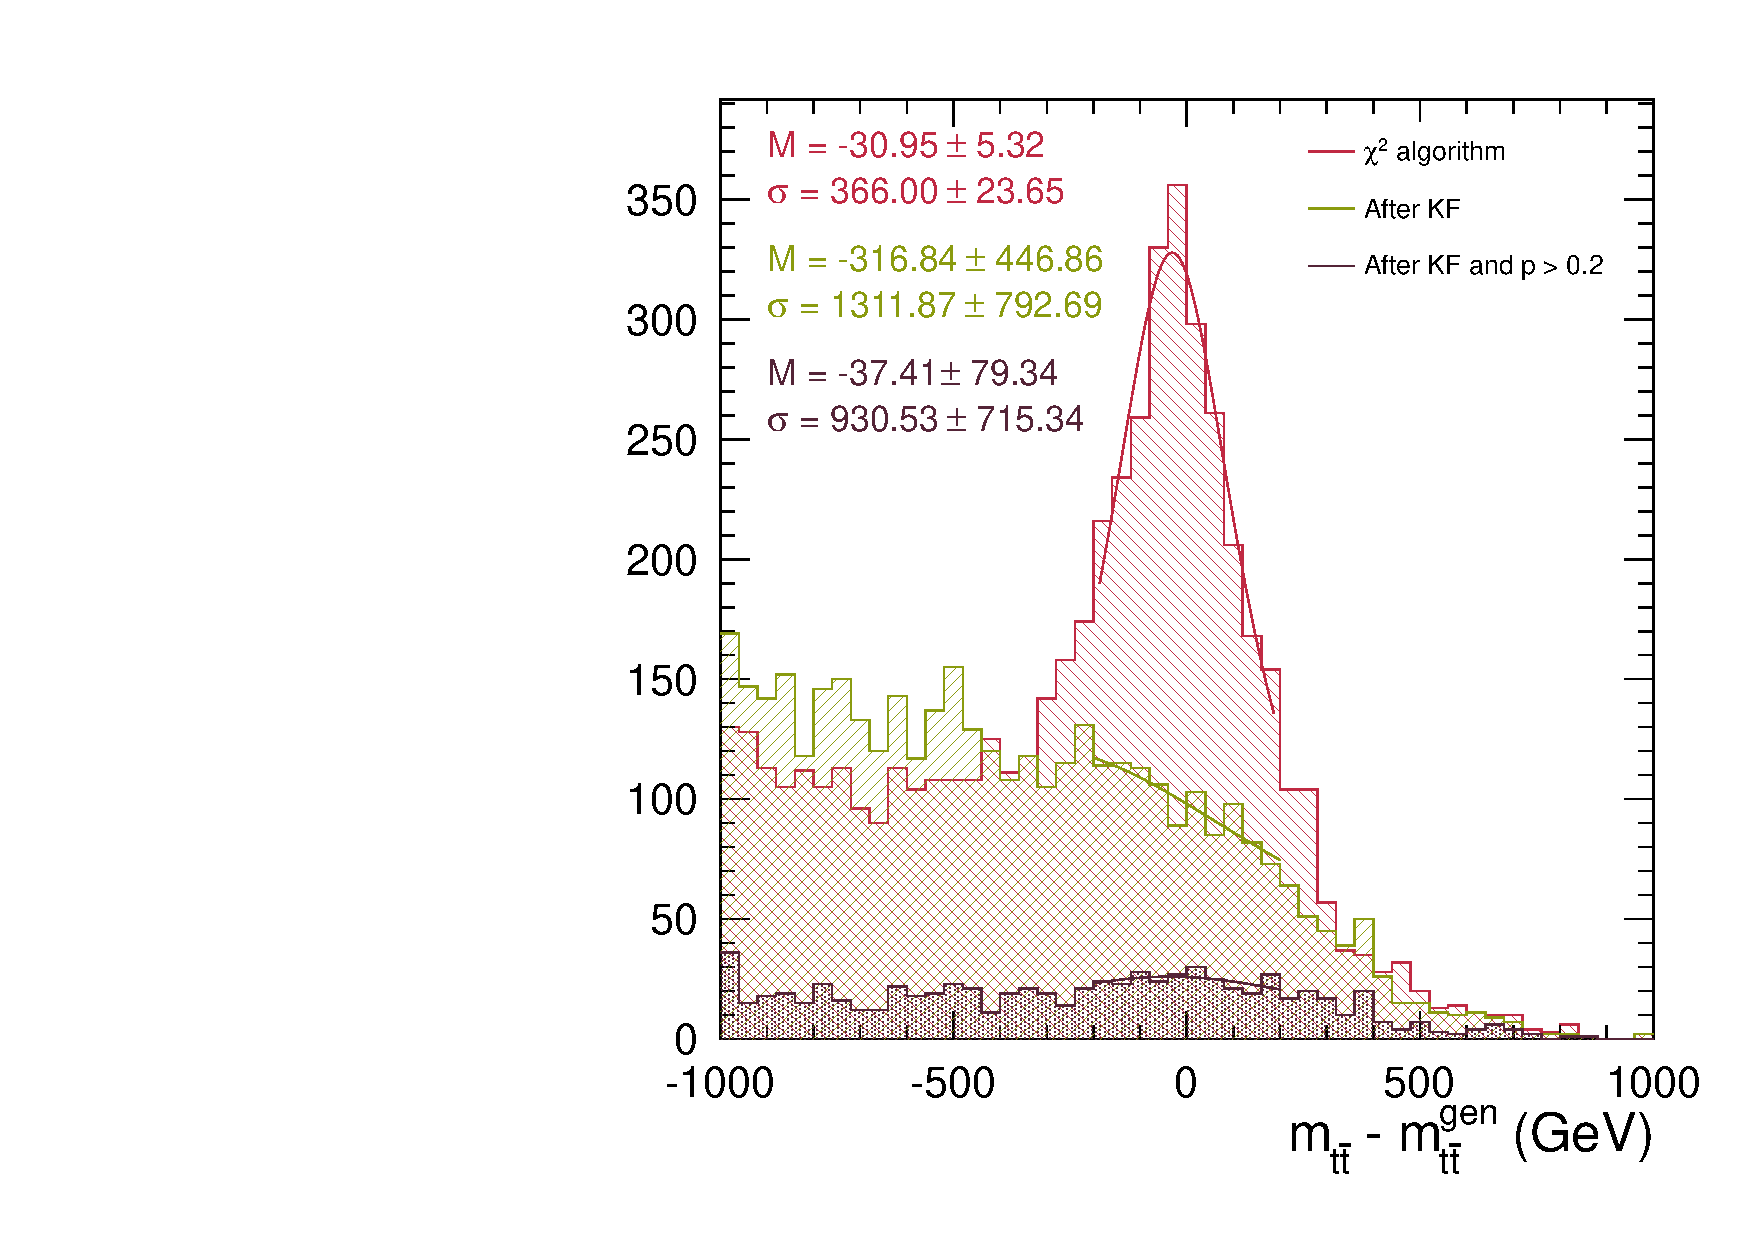
\includegraphics[width=0.48\textwidth,angle=-90,origin=c]{chapitre7/figs/kinfit/mtt_resolution_comparison_kf_zp2000_all_events.pdf}}
    \caption{Résolution sur \mtt avant (\rouge) et après (\vertc) utilisation de l'ajustement cinématique, pour un \zprime de masse $\mzp = \SI{750}{\GeV}$ (\subref{fig:kf_zp_750}) et $\mzp = \SI{2}{\TeV}$ (\subref{fig:kf_zp_2000}) en considérant tous les événements sélectionnés. Une coupure $p > \num{0.2}$ est appliquée pour obtenir la distribution \violette. Une interpolation par une Breit-Wigner est effectuée pour chaque distribution afin de faciliter la comparaison.}
    \label{fig:kf_zp}
\end{figure}

\subsubsection{L'ajustement cinématique} \label{sec:zprime_kf}

Les performances de l'ajustement cinématique ont été détaillées dans le \cref{chap:mtt_reco} pour des événements \ttbar Modèle Standard. Bien qu'on ai vu que la résolution était dégradée, cette section complète cette étude en incluant des événements \ttbar produits par des processus de nouvelle physique, plus particulièrement des \zprime.

\medskip

La \cref{fig:kf_zp} présente l'effet de l'ajustement cinématique sur la résolution de la masse invariante pour deux masses de \zprime, $\mzp = \SI{750}{\GeV}$ et $\mzp = \SI{2}{\TeV}$, dans l'hypothèse de résonances étroites. Comme on peut le voir sur ces distributions, l'effet de l'ajustement cinématique est catastrophique : la résolution est fortement dégradée, allant même jusqu'à faire disparaître le pic de résonance à \SI{2}{\TeV}. L'effet, déjà présent sur des événements \ttbar Modèle Standard, se trouve encore plus accentué sur des événements \ttbar produits par des processus de nouvelle physique. En effet, à \SI{500}{\GeV}, l'efficacité d'avoir un événement associable est comparable à celle du Modèle Standard (environ \SI{35}{\percent}), et chute à mesure que la masse augmente. Dans la \cref{sec:mtt_kf} on a vu que l'ajustement cinématique gère très mal les événements où la mauvaise combinaison de jet est sélectionnée, ce qui explique pourquoi les performances de l'ajustement cinématique sont comparables à celles sur des événements \ttbar du Modèle Standard pour un \zprime de \SI{500}{\GeV}, et très mauvaises à \SI{2}{\TeV}.

\subsection{Comparaisons données / simulation}

Afin de valider notre sélection, il est utile de procéder à quelques comparaisons entre les données et la simulation. On rappelle cependant qu'à aucun moment les événements simulés des bruits de fond ne sont utilisés dans la production des résultats finaux de cette analyse.

\medskip

\begin{figure}[p!] \centering
    \subcaptionbox{Canal semi-muonique}[0.49\textwidth]{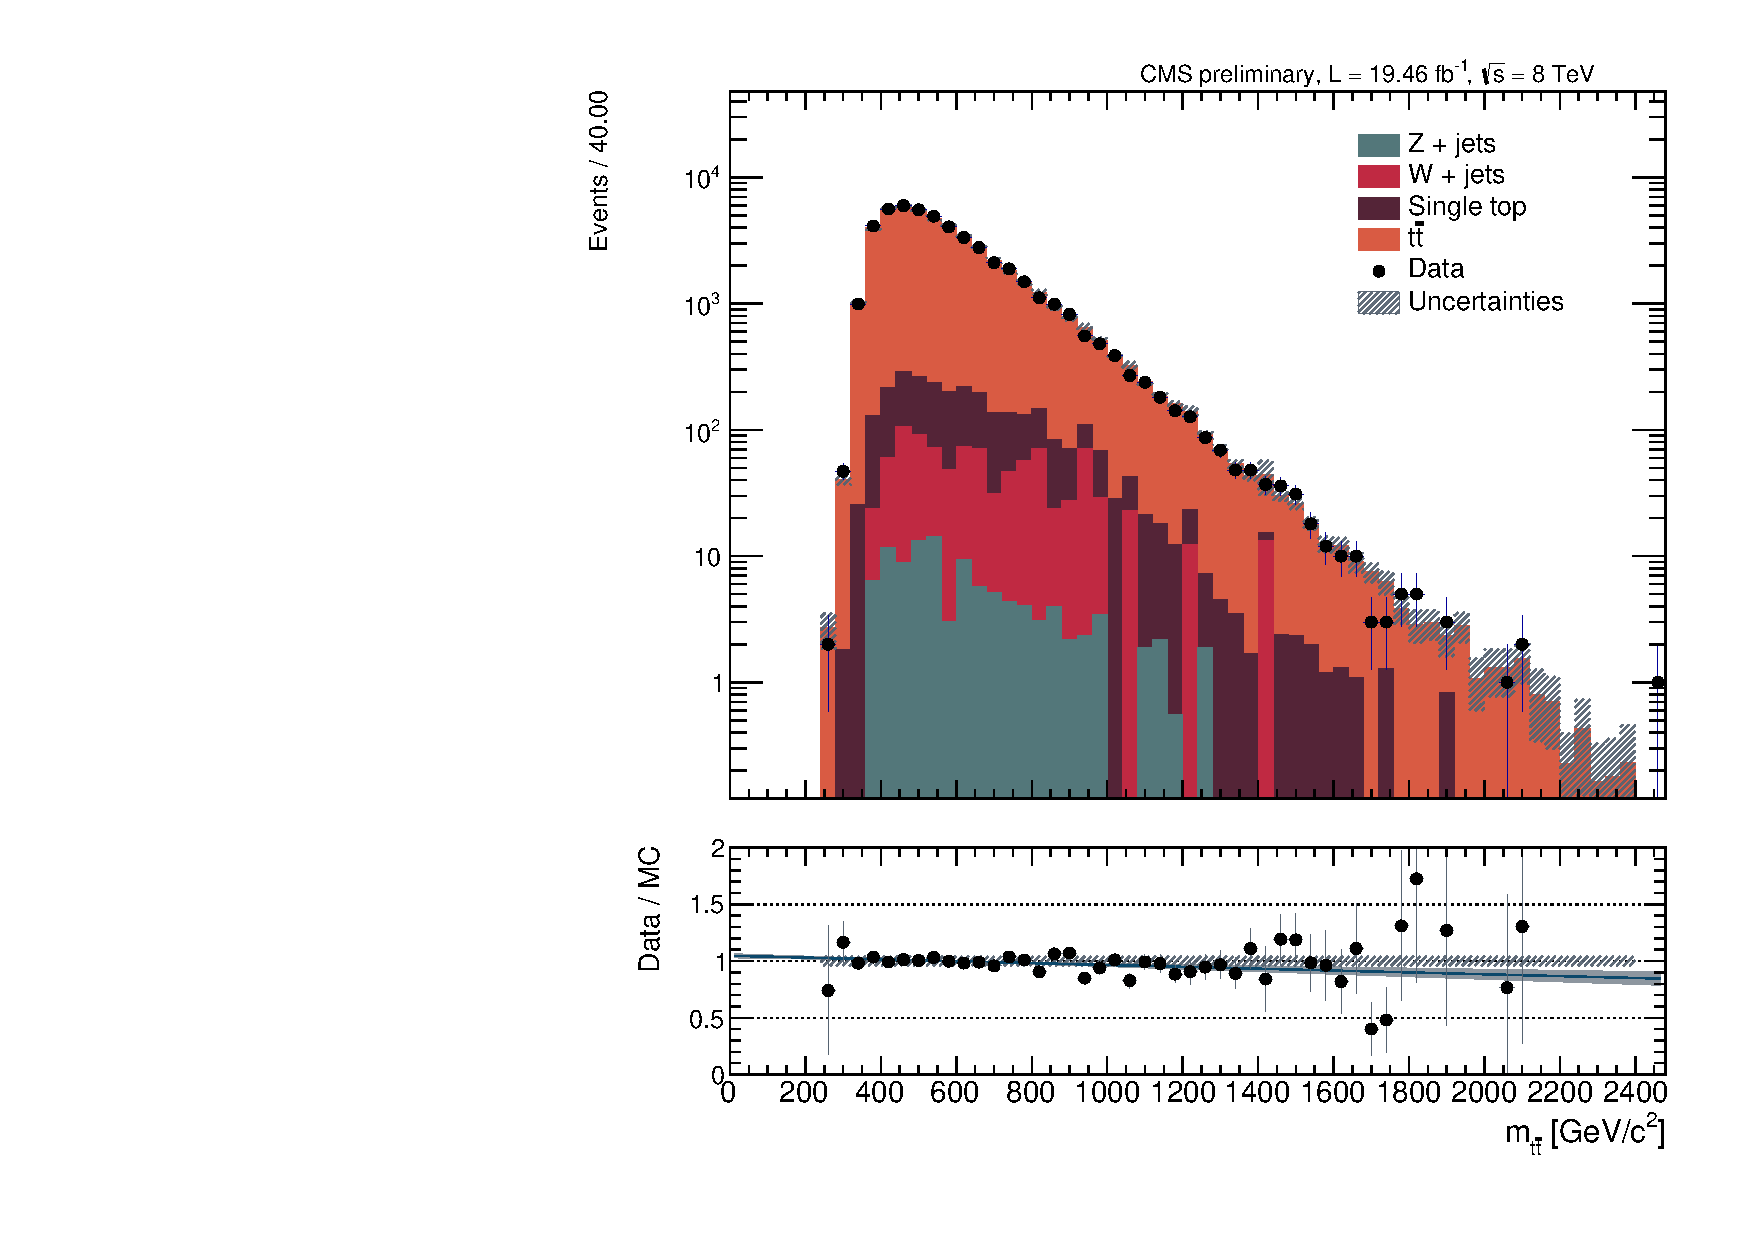
\includegraphics[width=0.49\textwidth,angle=-90,origin=c]{chapitre7/figs/data_mc/2btag/semimu/hmttSelected_btag_sel.pdf}} \hfill
    \subcaptionbox{Canal semi-électronique}[0.49\textwidth]{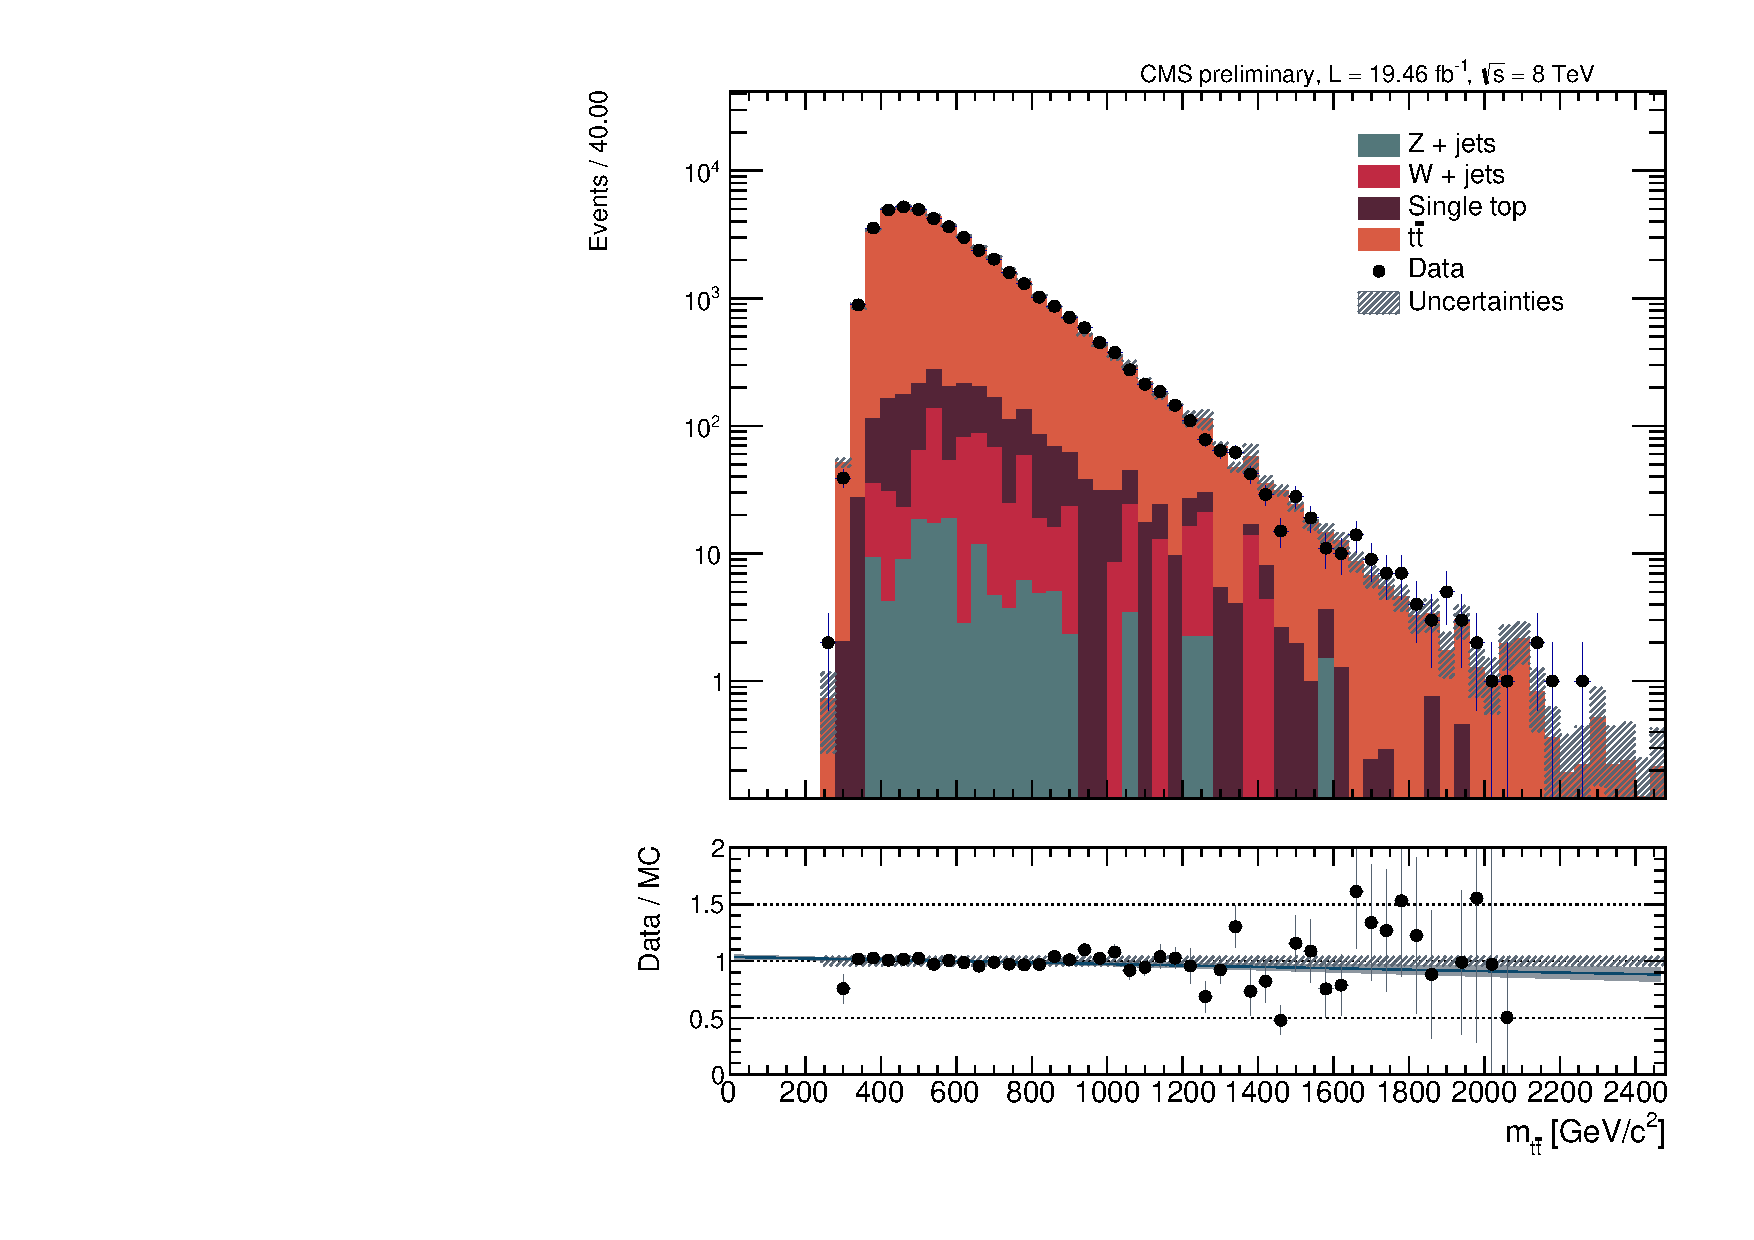
\includegraphics[width=0.49\textwidth,angle=-90,origin=c]{chapitre7/figs/data_mc/2btag/semie/hmttSelected_btag_sel.pdf}}
    \caption{Comparaison entre les données et la simulation, en sélectionnant au moins 2 jets étiquetés \Pbottom{}. Un ratio est présenté en bas de la distribution. La simulation est normalisée au nombre d'événements dans les données, et la zone hachurée correspond aux incertitudes statistiques.}
    \label{fig:data_mc_2b}
\end{figure}
 \begin{figure}[p!] \centering
    \subcaptionbox{Canal semi-muonique}[0.49\textwidth]{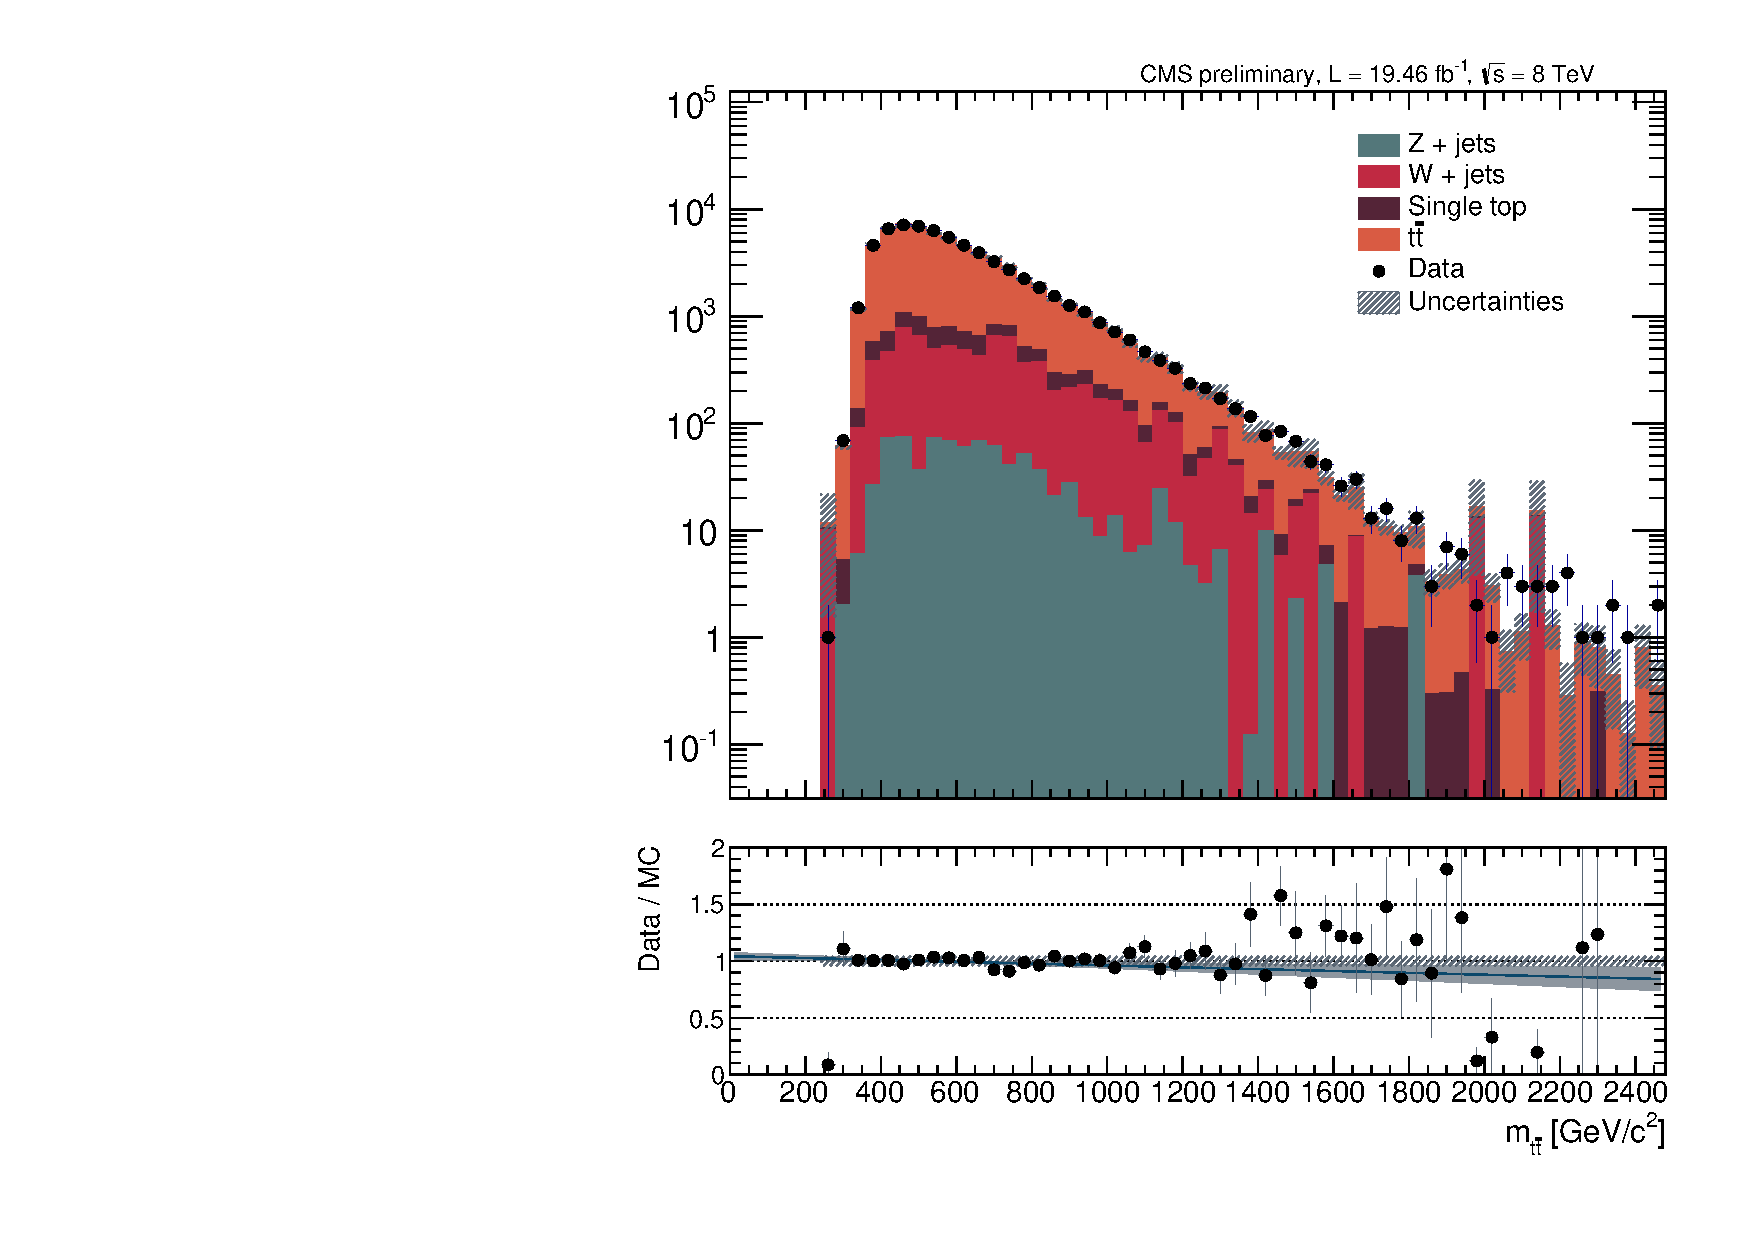
\includegraphics[width=0.49\textwidth,angle=-90,origin=c]{chapitre7/figs/data_mc/1btag/semimu/hmttSelected_btag_sel.pdf}} \hfill
    \subcaptionbox{Canal semi-électronique}[0.49\textwidth]{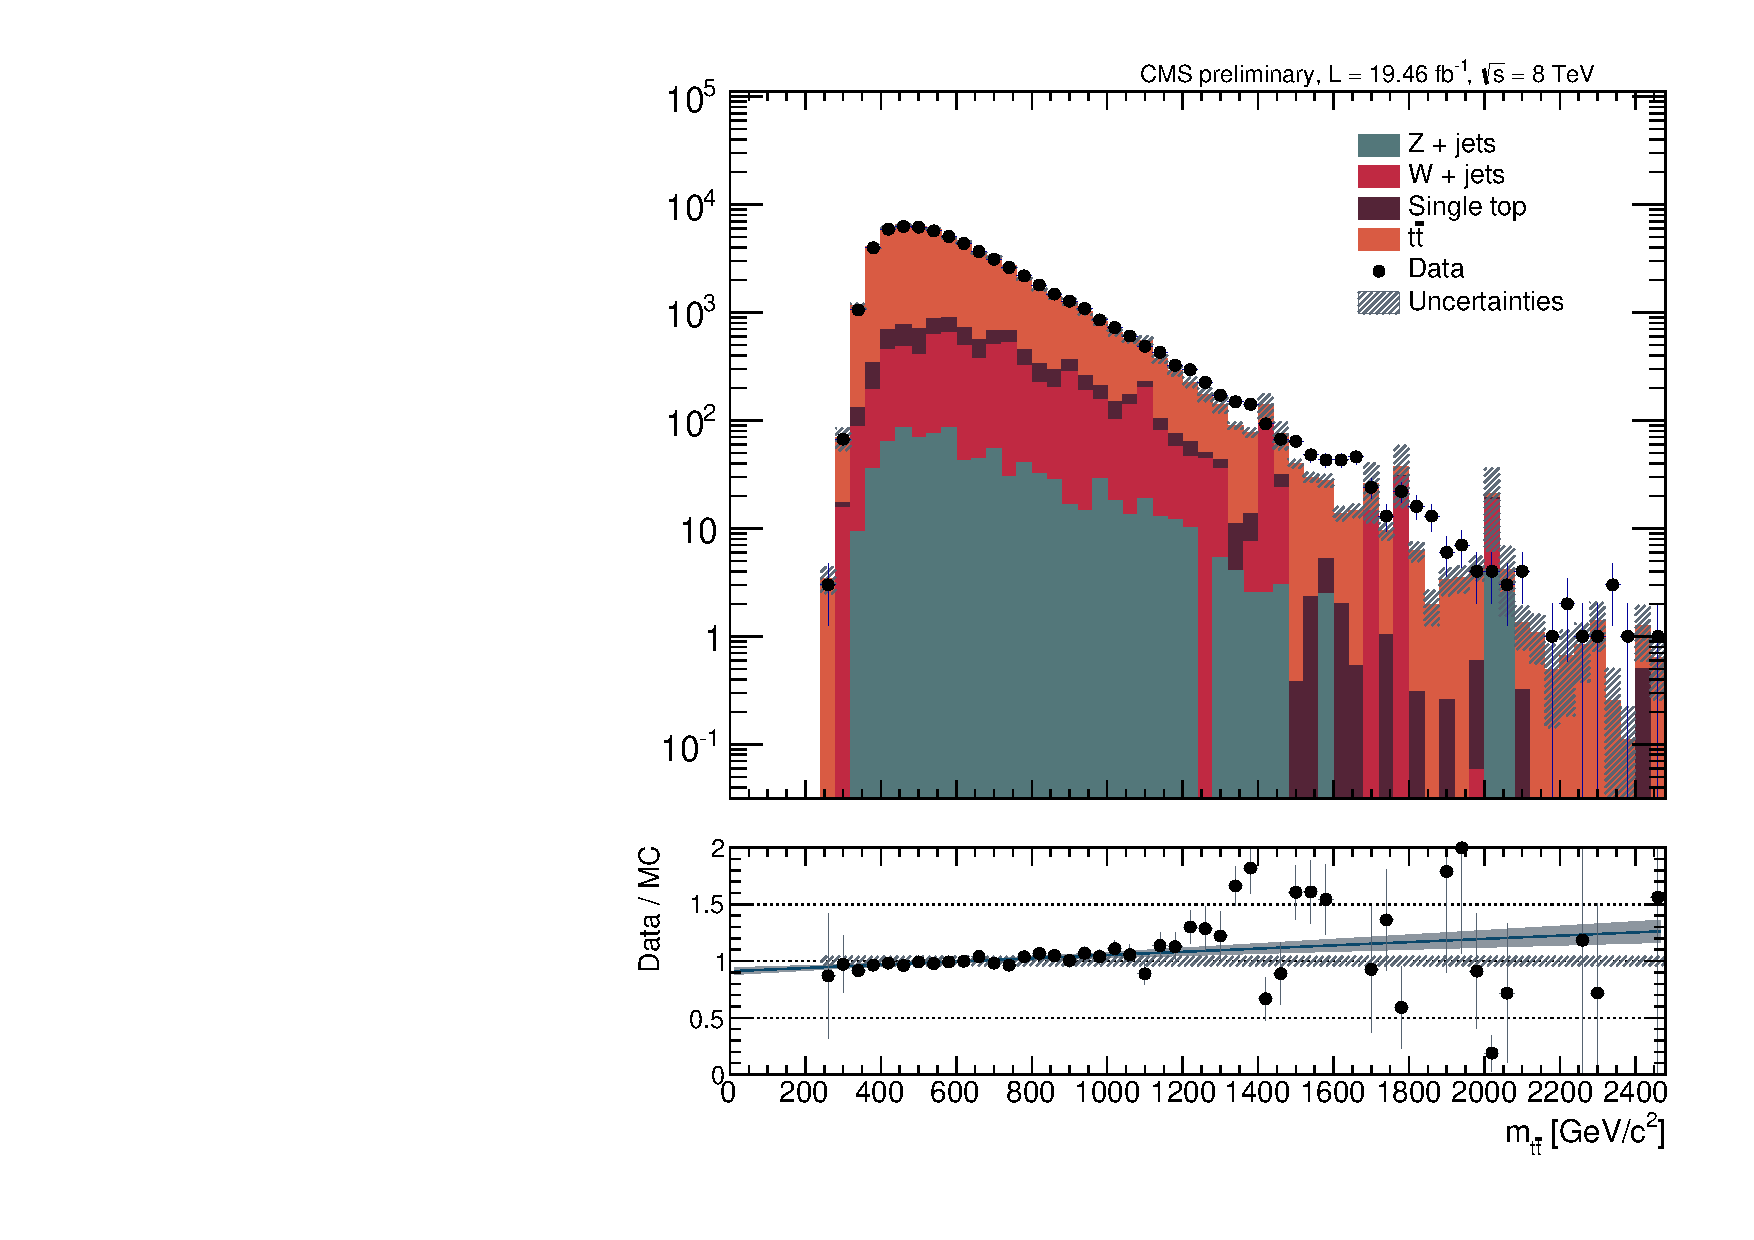
\includegraphics[width=0.49\textwidth,angle=-90,origin=c]{chapitre7/figs/data_mc/1btag/semie/hmttSelected_btag_sel.pdf}}
    \caption{Comparaison entre les données et la simulation, en sélectionnant exactement moins 1 jet étiqueté \Pbottom{}. Un ratio est présenté en bas de la distribution. La simulation est normalisée au nombre d'événements dans les données, et la zone hachurée correspond aux incertitudes statistiques.}
    \label{fig:data_mc_1b}
\end{figure}

La \cref{fig:data_mc_2b} présente la comparaison entre les données et la simulation pour \mtt, pour une sélection d'au moins 2 jets étiquetés \Pbottom, pour les canaux semi-muonique et semi-électronique. La simulation est normalisée au nombre d'événements dans les données. De façon analogue, la \cref{fig:data_mc_1b} présente la comparaison entre les données et la simulation, pour une sélection d'exactement 1 jet étiqueté \Pbottom. Les incertitudes présentées sur les distributions ne tiennent compte que des incertitudes statistiques ainsi que l'incertitude sur la luminosité totale collectée.

\medskip

Les \cref{tab:sel_perf_mu,tab:sel_perf_e} résument le nombre d'événements de fond attendu pour une luminosité intégrée de \SI{19.6}{\invfb}, après sélection et application des facteurs de corrections, pour toutes les catégories de l'analyse.

\begin{table}[thbp] \centering
\begin{tabular}{@{}ccccccc@{}} \toprule
  & \ttbar & \PW + jets & \PZ + jets & top célib. & total & données \\ \midrule
  1 jet étiqueté \Pbottom & 52238 & 7117 & 833 & 3238 & \num{63426 \pm 313} & 65475 \\
  + $\mtt > \SI{550}{\GeV}$ & 26037 & 4630 & 564 & 1910 & \num{33140 \pm 249} & 34175 \\ \midrule
  2 jets étiquetés \Pbottom & 43774 & 821 & 104 & 1848 & \num{46547 \pm 133} & 48653 \\
  + $\mtt > \SI{550}{\GeV}$ & 20190 & 559 & 54 & 1102 & \num{21905 \pm 101} & 22561 \\ \bottomrule
\end{tabular}
\caption{Nombre d'événements de fonds attendus pour une luminosité de \SI{19.6}{\invfb} et pour le canal semi-muonique, après application de tous les facteurs de corrections sur la simulation. L'incertitude est uniquement statistique, et la simulation est normalisée grâce aux sections efficaces de production théoriques.}
\label{tab:sel_perf_mu}
\end{table}

\begin{table}[thbp] \centering
\begin{tabular}{@{}ccccccc@{}} \toprule
  & \ttbar & \PW + jets & \PZ + jets & top célib. & total & données \\ \midrule
  1 jet étiqueté \Pbottom & 46147 & 5639 & 802 & 2788 & \num{55491 \pm 288} & 60690 \\
  + $\mtt > \SI{550}{\GeV}$ & 23167 & 4110 & 515 & 1693 & \num{29485 \pm 240} & 32940 \\ \midrule
  2 jets étiquetés \Pbottom & 43213 & 747 & 137 & 1834 & \num{445932 \pm 141} & 43088 \\
  + $\mtt > \SI{550}{\GeV}$ & 17536 & 433 & 67 & 985 & \num{19459 \pm 93} & 20291 \\ \bottomrule
\end{tabular}
\caption{Nombre d'événements de fonds attendus pour une luminosité de \SI{19.6}{\invfb} et pour le canal semi-électronique, après application de tous les facteurs de corrections sur la simulation. L'incertitude est uniquement statistique, et la simulation est normalisée grâce aux sections efficaces de production théoriques.}
\label{tab:sel_perf_e}
\end{table}

Le nombre d'événements de fond attendus est systématiquement plus bas que le nombre d'événement observés sur les données. Cette différence peut être expliquée par le fait que le fond multi-jets n'est pas pris en compte dans les chiffres présentés ci-dessous. Afin de conforter cette hypothèse, la distribution de l'énergie manquante pour le canal semi-électronique est présentée sur la \cref{fig:data_mc_met}. Sur cette distribution, le désaccord entre la simulation et les données est principalement visible à bas \met, là où les événements multi-jets sont principalement localisés. En appliquant une coupure supplémentaire sur \met, $\met > \SI{80}{\GeV}$, le nombre d'événements de fond attendus dans ce canal devient \num{16682 \pm 136}, à comparer aux \num{16634} événements de données observés. Le désaccord observé est donc dû à l'absence du fond simulé multi-jets.

\begin{figure}[tbp]
  \centering
  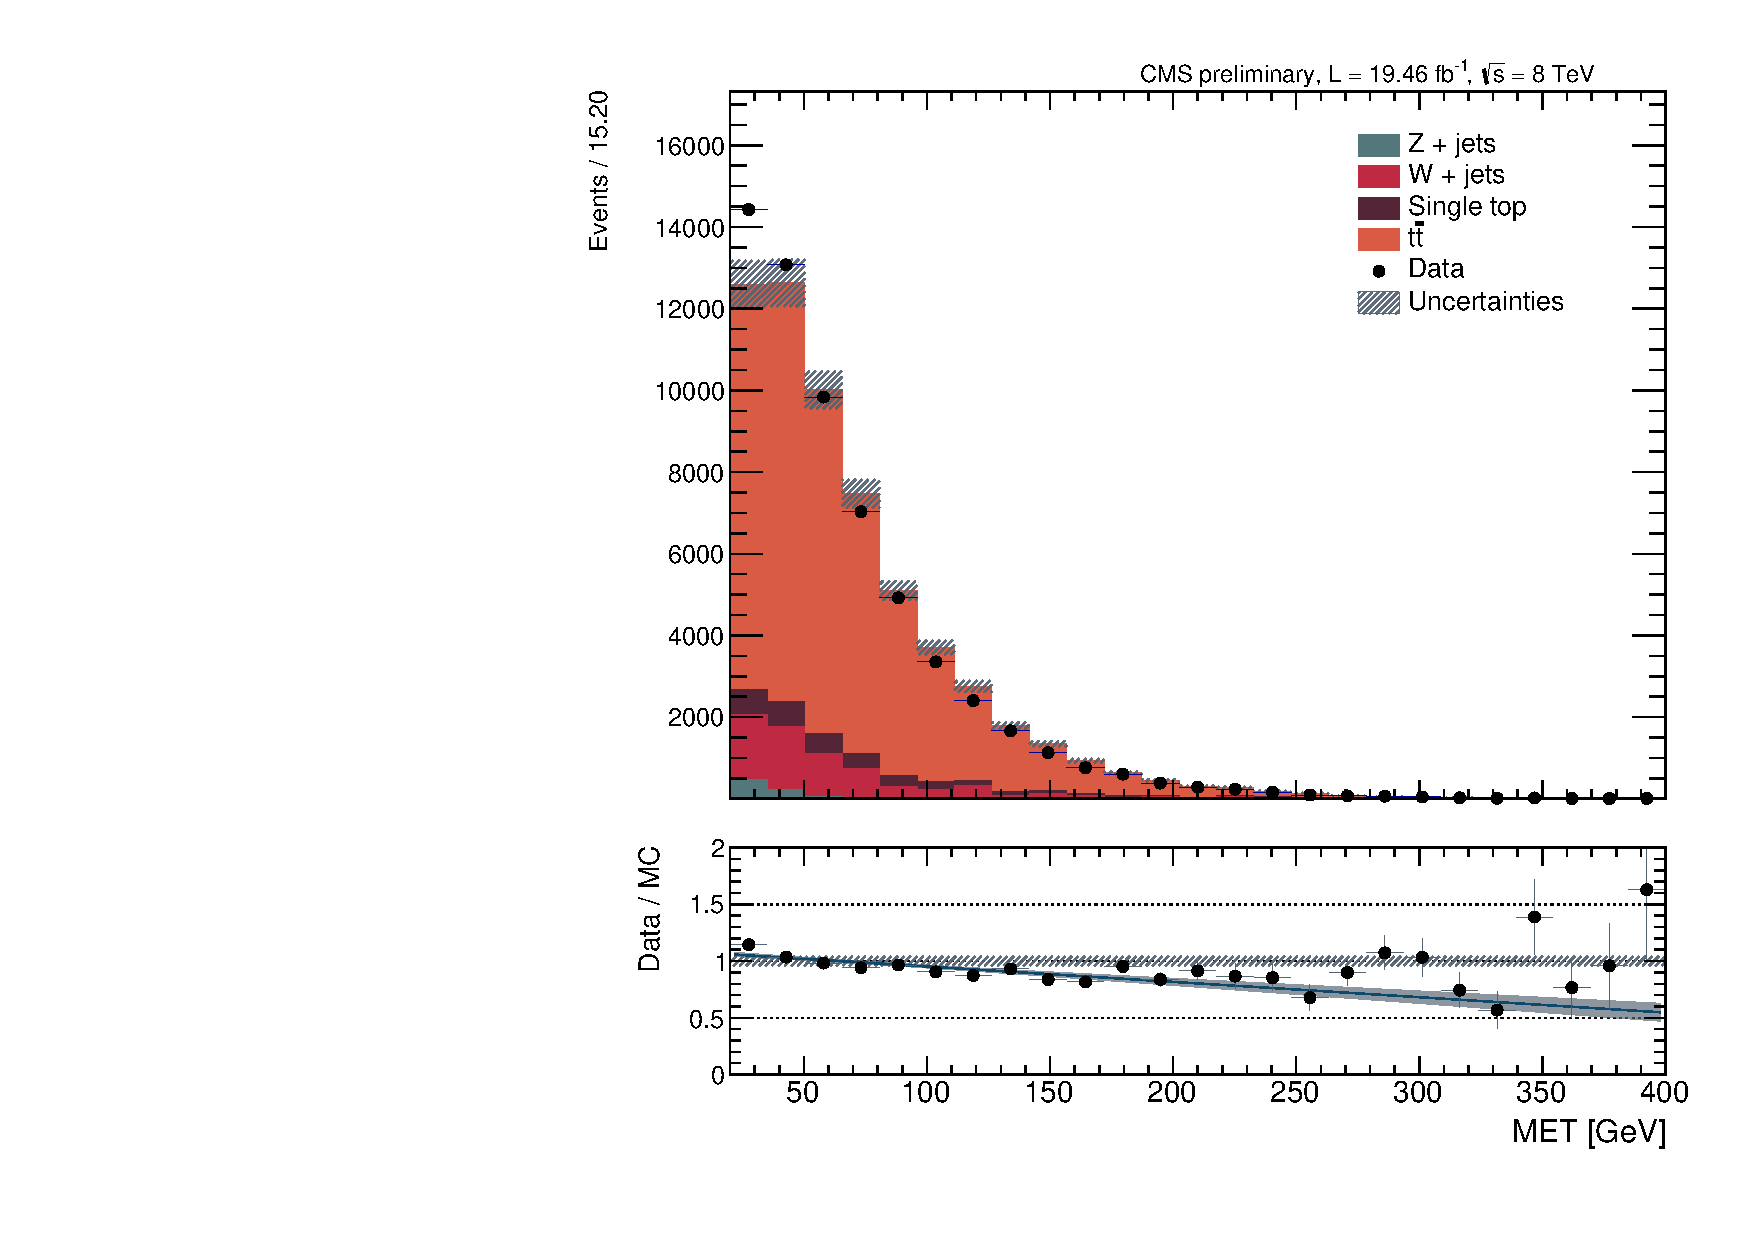
\includegraphics[width=0.48\textwidth,angle=-90,origin=c]{chapitre7/figs/data_mc/1btag/semie/hMET.pdf}
  \caption{Distribution de l'énergie transverse manquante pour le canal semi-électronique, en sélectionnant uniquement des événements avec uniquement 1 jet étiqueté \Pbottom. Le désaccord à bas \met est dû à l'absence du fond multi-jets.}
  \label{fig:data_mc_met}
\end{figure}

\section{Analyse statistique} \label{sec:stat}

On souhaite extraire le nombre d'événements de signal présent dans les données. On définit pour cela deux densités de probabilités (PDF), une permettant de décrire le bruit de fond, et une permettant de décrire la résonance. Ces deux fonctions sont ensuite sommées afin de fournir une PDF globale, utilisée ensuite pour ajuster les données. La procédure d'ajustement est décrite dans la prochaine section, et le choix des PDFs associées au fond et signal dans les sections suivantes.

\subsection{Structure de l'ajustement}

On dispose de deux PDFs, décrivant respectivement le fond et le signal. Ces PDFs, si elles sont analytiques, possèdent des paramètres libres, qu'on souhaite estimer sur les données pour le fond et sur la simulation pour le signal, en plus de la normalisation respective de chaque fonction. On réalise ainsi un ajustement utilisant la méthode du maximum de vraisemblance. La fonction de vraisemblance $\mathcal{L}$ est définie par
\begin{align*}
  \mathcal{L}(\mtt \mid \theta) &= \prod\limits_{i = 0}^B \left( \frac{\mu_i(\mtt^i \mid \theta)^{n_i} \, e^{- \mu_i(\mtt^i \mid \theta)}}{n_i!} \right) \\
  \mu_i(\mtt^i \mid \theta) &= N_S^i \; f_S(\mtt^i \mid \theta) + N_B^i \; f_B(\mtt^i \mid \theta)
\end{align*}
où $\theta$ symbolise l'ensemble des paramètres libres des PDFs, $B$ le nombre de classes en \mtt, $n_i$ le nombre d'événements dans la classe $i$, $N_S$ ($N_B$) le nombre d'événements de signal (de fond), et $f_S(\mtt^i \mid \theta)$ ($\;f_B(\mtt^i \mid \theta)\;$) la PDF décrivant le signal (le fond). Maximiser $\mathcal{L}$ permet d'obtenir les valeurs $\hat{\theta}$, $\hat{N_S}$ et $\hat{N_B}$ les plus probables, c'est-à-dire qui permettent d'obtenir la description optimale des données. Le nombre de classes en \mtt est fixé de façon à ce que chaque classe ait une largeur de \SI{4}{\GeV}.

\medskip

Les événements sélectionnés par l'analyse sont classés dans 4 catégories, selon le nombre de jets étiquetés \Pbottom et la saveur du lepton. Si un signal de nouvelle physique est présent, il doit apparaître de façon cohérente dans chacune des catégories. On effectue un ajustement simultané, en ajoutant comme contrainte que le nombre d'événements de signal dans chaque catégorie soit compatible avec l'efficacité de sélection dans cette catégorie. Lors de l’ajustement, les paramètres de la PDF décrivant le signal sont fixés aux valeurs déterminées sur la simulation, tandis que ceux de la PDF décrivant le fond sont libres de varier. Les PDFs du fond et du signal sont obtenues séparément pour chacune des catégories considérées dans l'analyse.

\bigskip

Une fois l'ajustement effectué, on peut extraire la section efficace de production de nouvelle physique en utilisant le nombre d'événements de signal déterminé par l'ajustement. On a
\begin{align} \label{eq:cross_section}
  \sigma &= \frac{\hat{N_S}}{\mathcal{L} \; \epsilon_{\text{sélection}}}
\end{align}
où $\mathcal{L}$ est ici la luminosité intégrée collectée, et $\epsilon_{\text{sélection}}$ l'efficacité de sélection du signal.

\subsection{Choix de la PDF de signal}

% \begin{figure}[tbp] \centering
%     \subcaptionbox{Exactement 1 jet étiqueté \Pbottom.}[0.99\textwidth]{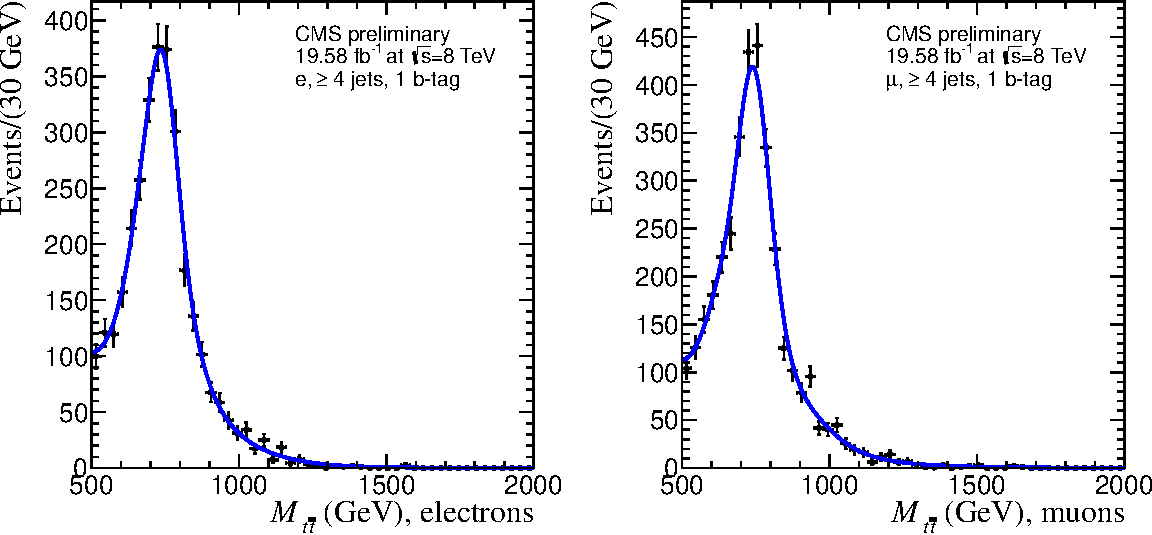
\includegraphics[width=0.99\textwidth]{chapitre7/figs/signal/nominal-Zprime750_keysPdf_1_btag.pdf}} \\ \vspace{5mm}
%     \subcaptionbox{Au moins 2 jets étiquetés \Pbottom.}[0.99\textwidth]{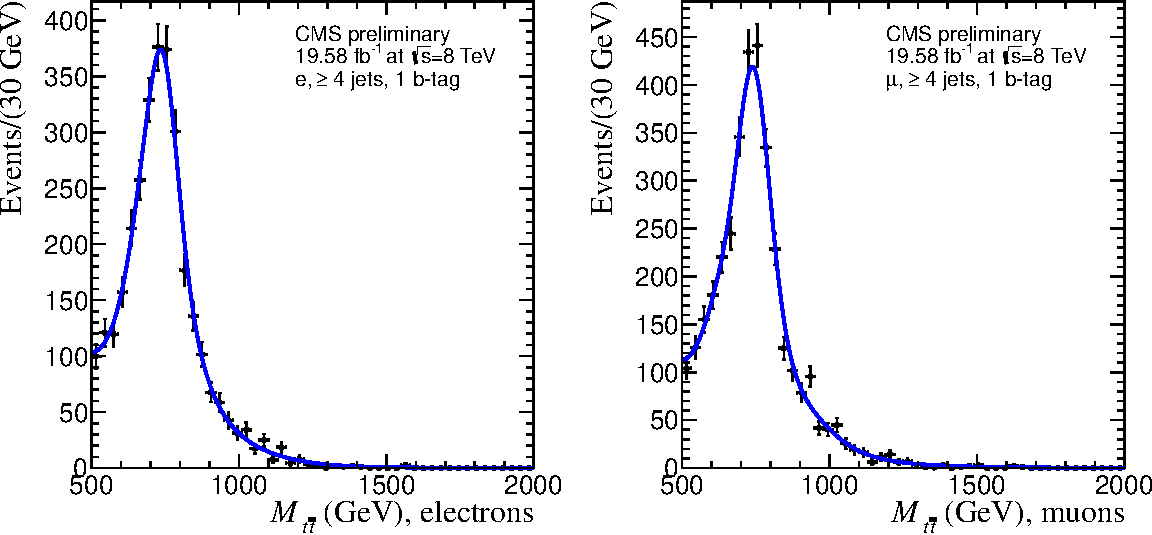
\includegraphics[width=0.99\textwidth]{chapitre7/figs/signal/nominal-Zprime750_keysPdf_1_btag.pdf}}
%     \caption{Distributions de masse invariante de paires \ttbar pour un \zprime de masse $\mzp = \SI{750}{\GeV}$, dans l'hypothèse de résonances étroites, pour le canal semi-électronique (gauche) et le canal semi-muonique (droite). Une interpolation par noyaux gaussiens est superposée.}
%     \label{fig:label}
% \end{figure}

\begin{figure}[tbp] \centering
    \subcaptionbox{Canal semi-muonique, au moins 2 jets étiquetés \Pbottom.}[0.48\textwidth]{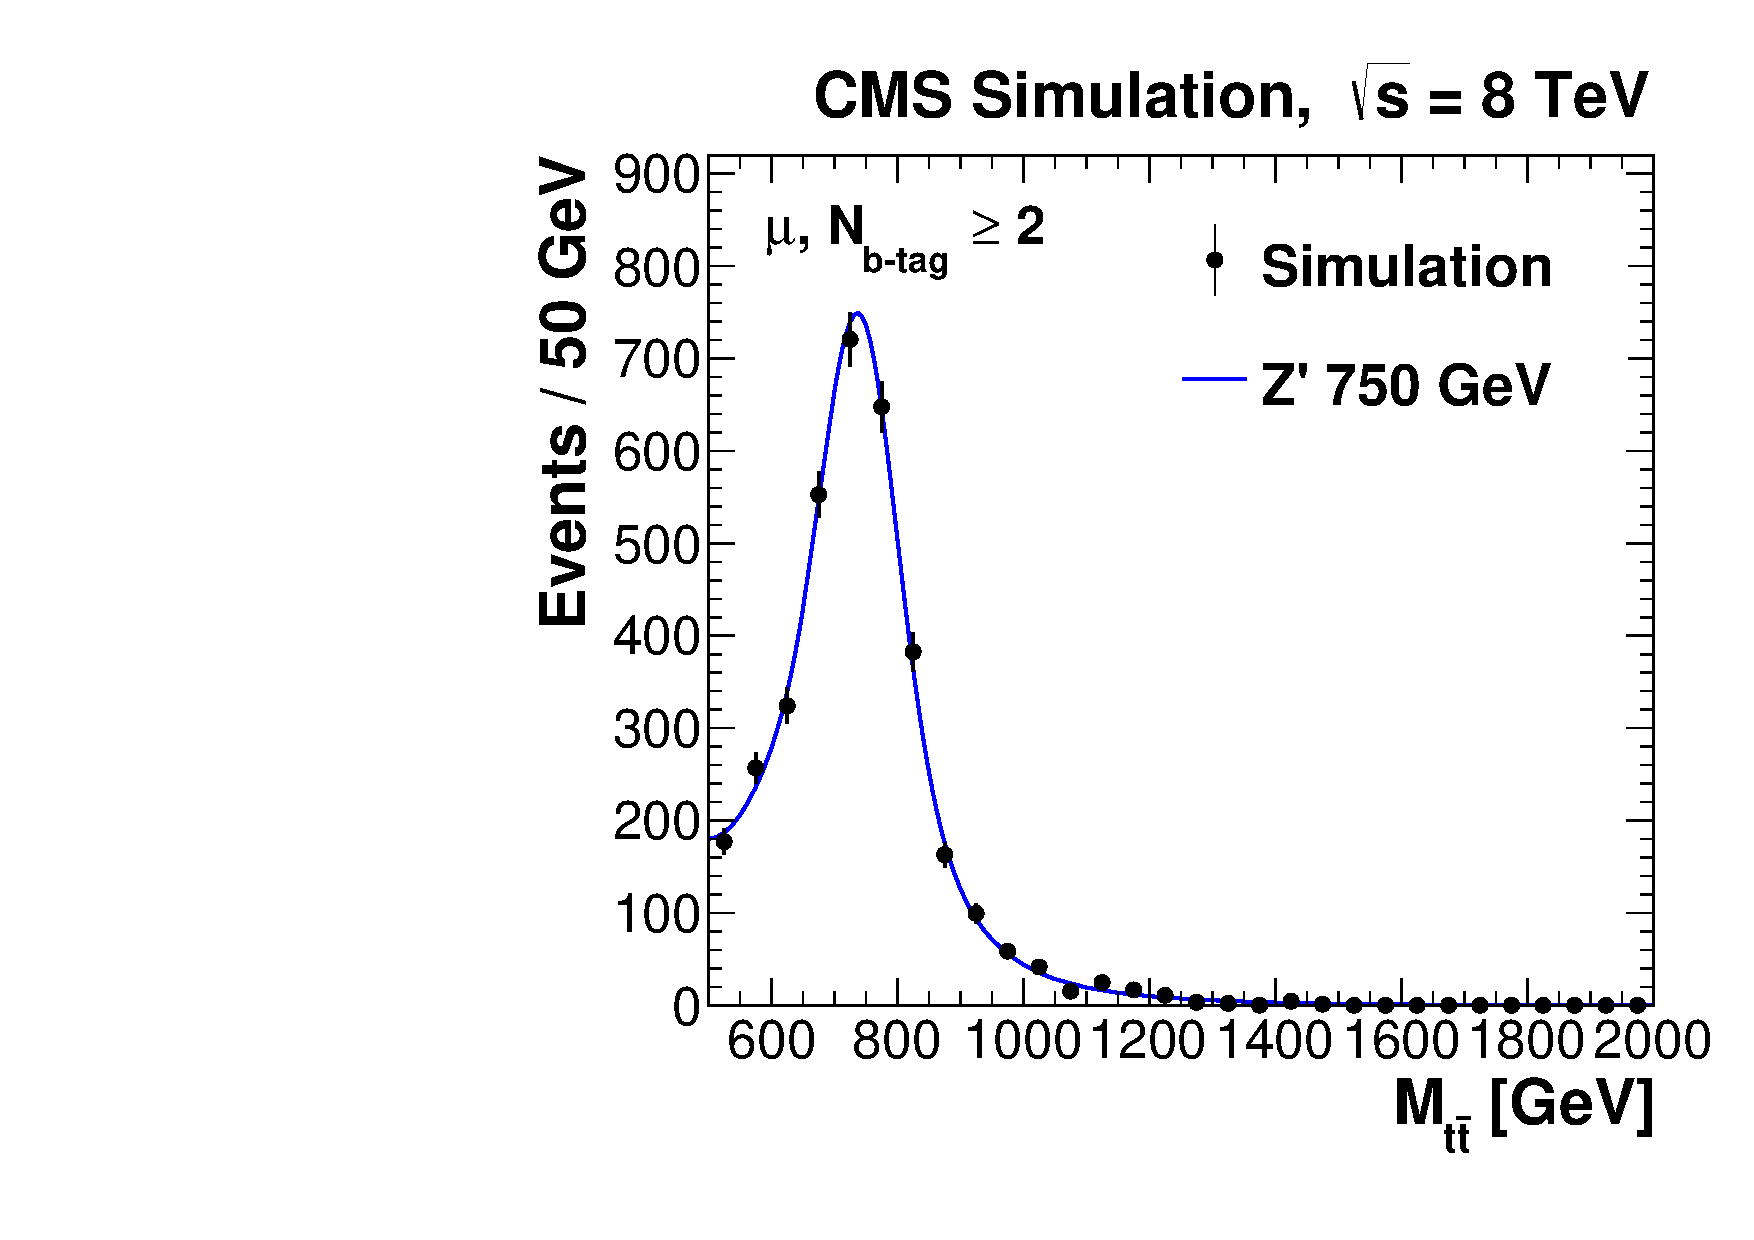
\includegraphics[width=0.48\textwidth,angle=-90,origin=c]{chapitre7/figs/signal/signal_zprime_750_mu_2b.pdf}} \hfill
    \subcaptionbox{Canal semi-électronique, au moins 2 jets étiquetés \Pbottom.}[0.48\textwidth]{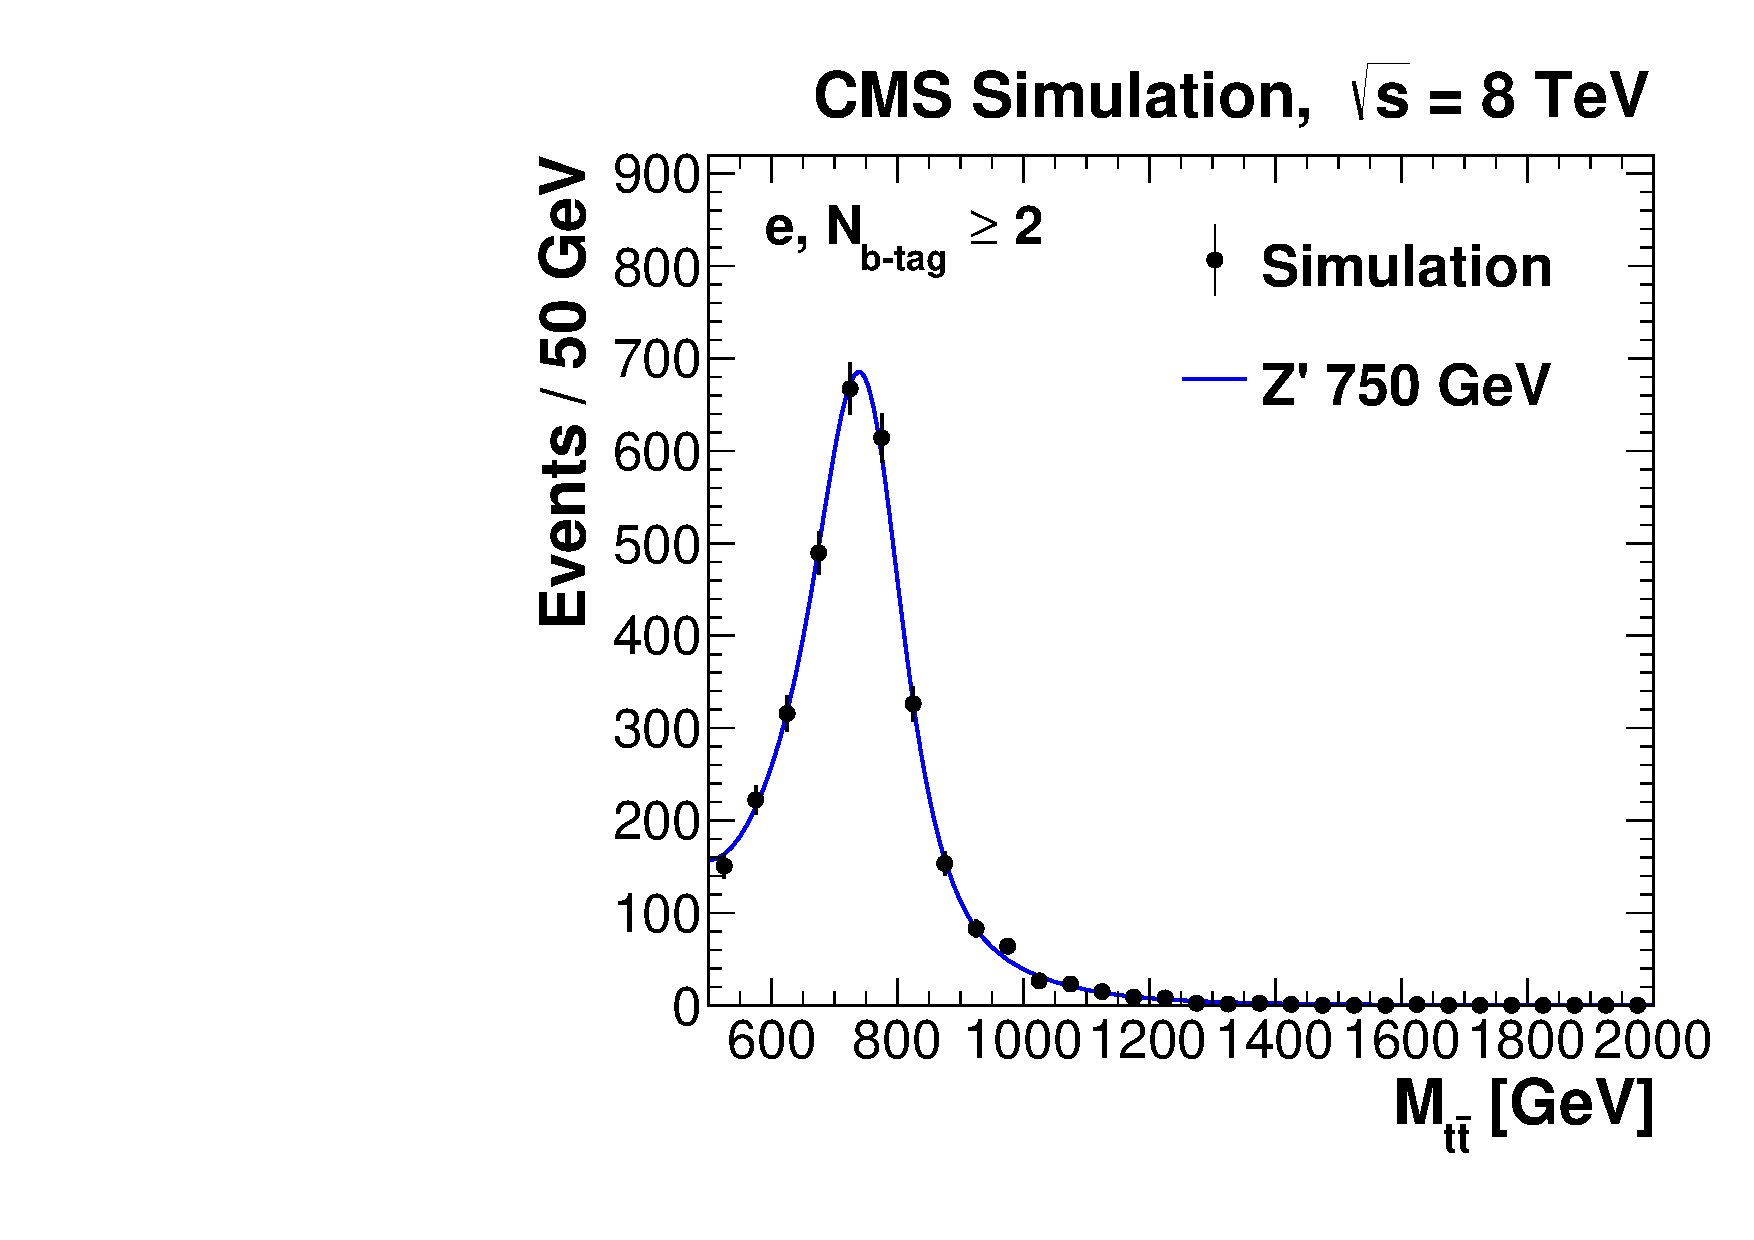
\includegraphics[width=0.48\textwidth,angle=-90,origin=c]{chapitre7/figs/signal/signal_zprime_750_e_2b.pdf}} \\
    \subcaptionbox{Canal semi-muonique, exactement 1 jet étiqueté \Pbottom.}[0.48\textwidth]{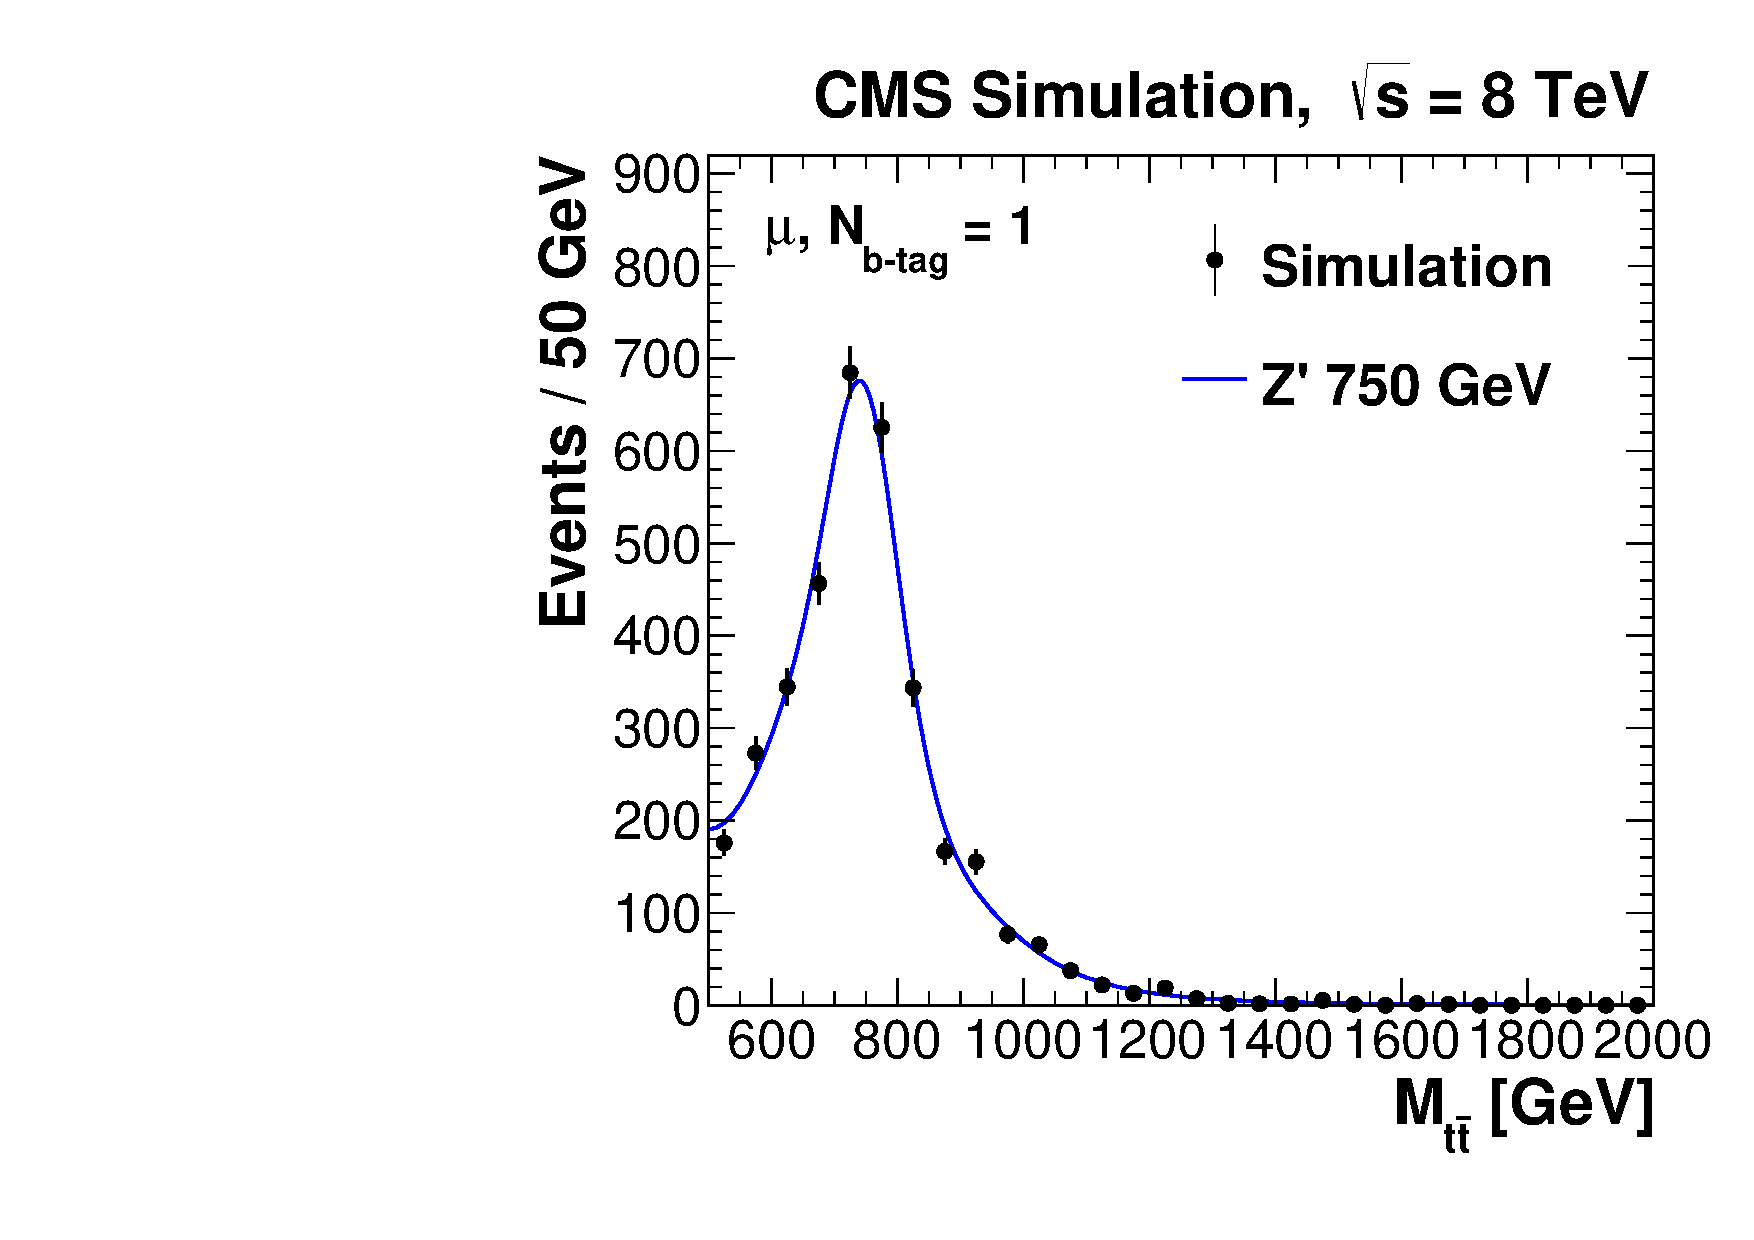
\includegraphics[width=0.48\textwidth,angle=-90,origin=c]{chapitre7/figs/signal/signal_zprime_750_mu_1b.pdf}} \hfill
    \subcaptionbox{Canal semi-électronique, exactement 1 jet étiqueté \Pbottom.}[0.48\textwidth]{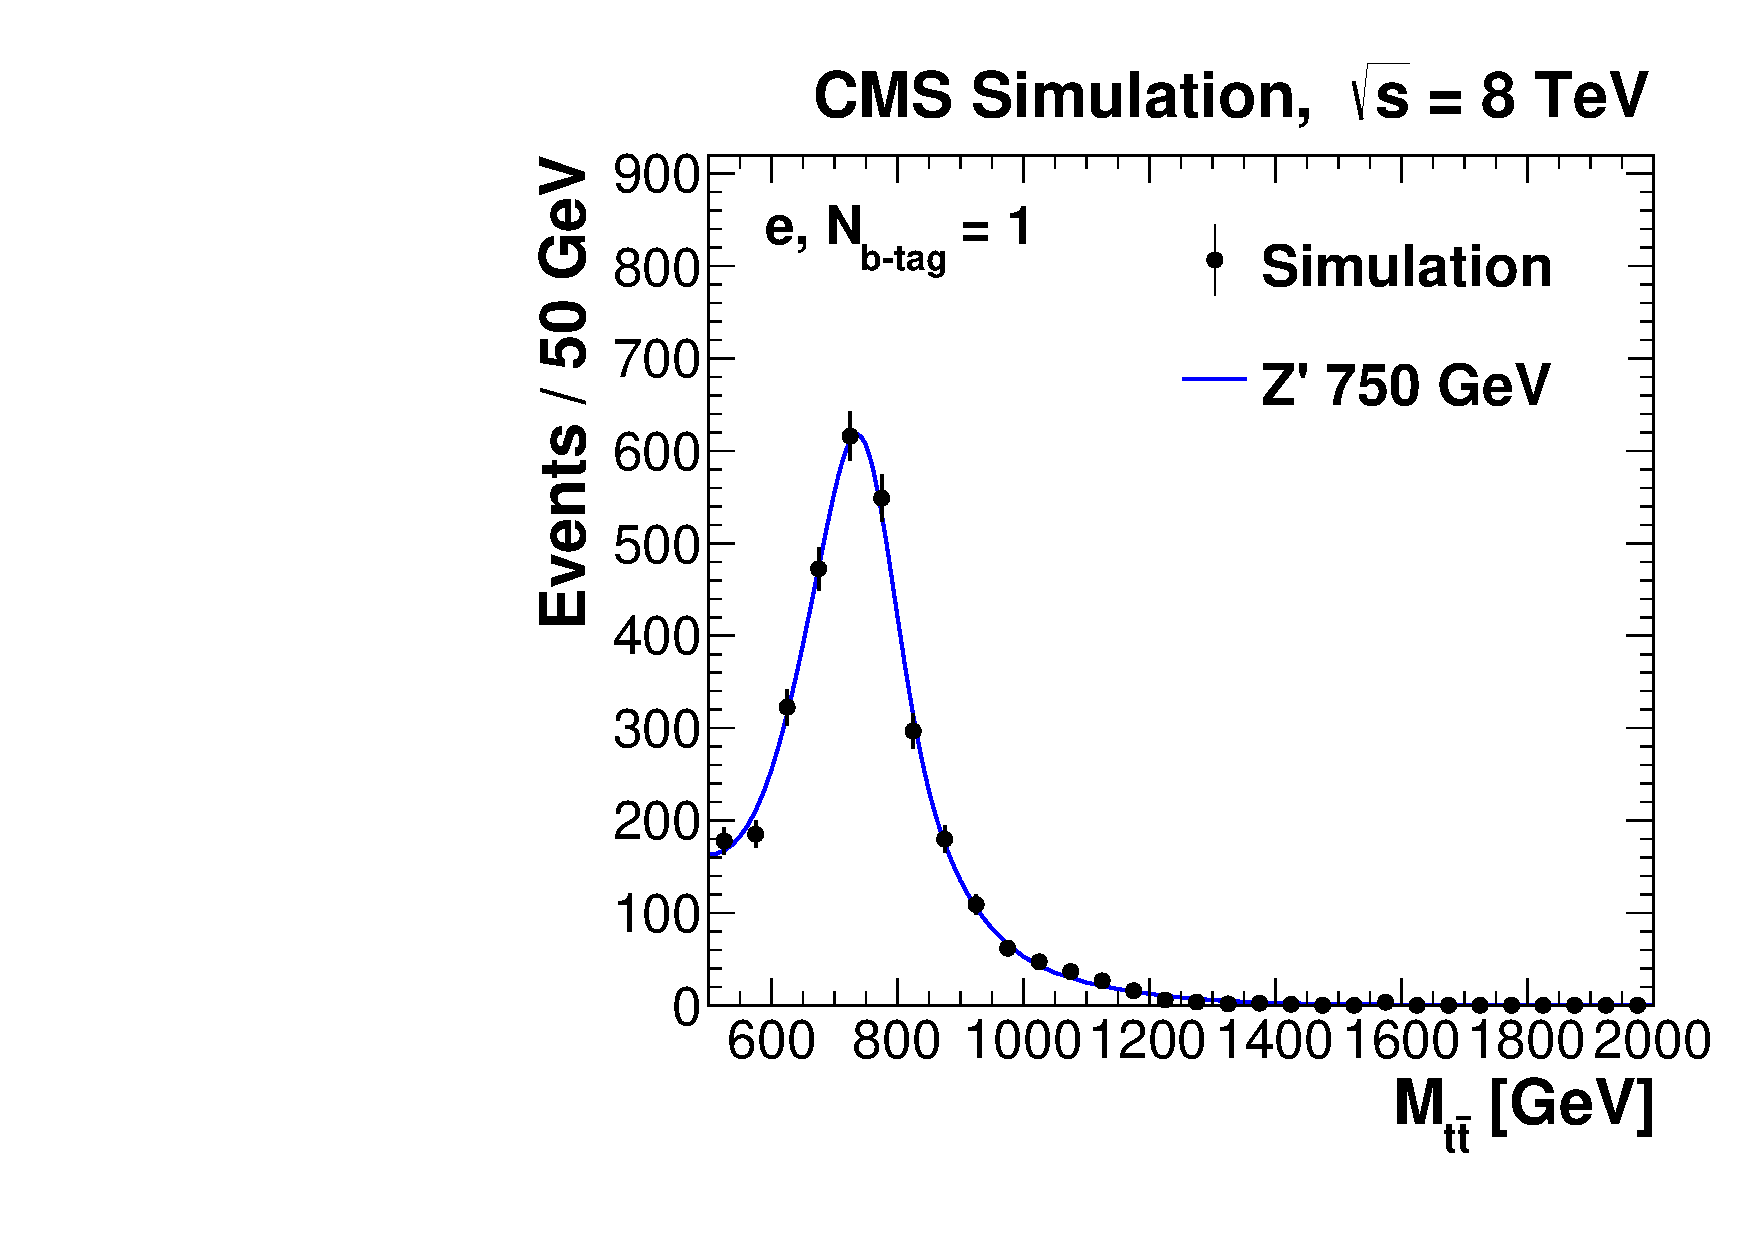
\includegraphics[width=0.48\textwidth,angle=-90,origin=c]{chapitre7/figs/signal/signal_zprime_750_e_1b.pdf}}
    \caption{Distributions de masse invariante de paires \ttbar pour un \zprime de masse $\mzp = \SI{750}{\GeV}$, dans l'hypothèse de résonances étroites. Une interpolation par noyaux gaussiens est superposée.}
    \label{fig:signal_pdf}
\end{figure}

Le signal est décrit en utilisant une interpolation par noyaux gaussiens \citep{Cranmer:2000du}. Cette méthode est préférée à une interpolation analytique principalement parce que la forme de signal change en fonction de la masse de la résonance. Il est ainsi difficile de trouver une forme analytique qui marche aussi bien à basse masse qu'à haute masse. Des tentatives ont été faites en utilisant une fonction Crystal-Ball, mais la description du signal n'était pas satisfaisante.

\medskip

La \cref{fig:signal_pdf} présente les distributions de masse invariante pour un \zprime de masse $\mzp = \SI{750}{\GeV}$, pour toutes les catégories de l'analyse. L'interpolation par noyaux gaussiens est superposée sur chaque distribution. Il est important de noter que l'interpolation par noyaux gaussiens n'est pas une fonction analytique : la PDF ainsi obtenue ne possède aucun paramètre libre.

\subsection{Choix de la PDF du fond} \label{sec:zp_bkg_pdf}

Le signal se manifeste sous la forme d'une résonance dans un spectre de masse décroissant. On cherche ainsi une fonction analytique strictement décroissante. Parmi plusieurs formes, on sélectionne la fonction qui biaise le moins l'analyse : en cas de présence de signal, la fonction décrivant le fond ne doit pas être en mesure d'absorber ce signal. Pour cela, plusieurs études ont été effectuée, décrites dans la suite de cette section.

\medskip

Trois fonctions sont considérées, inspirées des fonctions de distributions partoniques :
\begin{align}
  \frac{\mathrm{d}\sigma}{\mathrm{d}\mtt} &= \frac{\left( 1 - \frac{m}{\sqrt{s}} + c_3 \left( \frac{m}{\sqrt{s}} \right)^2 \right)^{c_1}}{m^{c_2}} \tag{PDF-A} \label{pdfA} \\
  \frac{\mathrm{d}\sigma}{\mathrm{d}\mtt} &= \frac{\left( 1 - \frac{m}{\sqrt{s}} \right)^{c_1} }{ \left( \frac{m}{\sqrt{s}}  \right)^{c_2 + c_3\ln{m / \sqrt{s}}}} \tag{PDF-B} \label{pdfB} \\
  %\frac{\mathrm{d}\sigma}{\mathrm{d}\mtt} &= \frac{\left( 1 - \frac{m}{\sqrt{s}} \right)^{c_1} }{ m^{c_2} } \tag{PDF-C}
  \frac{\mathrm{d}\sigma}{\mathrm{d}\mtt} &= \frac{1}{1 + \exp{\frac{m / \sqrt{s} - c_1}{c_2}}} \tag{PDF-C} \label{pdfC}
\end{align}

Lors de l'ajustement sur les données, la même fonction est utilisée pour chacune des catégories de l'analyse. Néanmoins, les paramètres de cette fonction sont indépendants dans chaque catégorie.

\begin{table} \centering
\begin{tabular}{@{}cccc@{}} \toprule
 & \ref{pdfA} & \ref{pdfB} & \ref{pdfC} \\ \midrule
 $\chi^2 \, / \, NdL$ & \num{1.0515} & \num{1.0520} & \num{1.0520} \\
 \bottomrule
\end{tabular}
\caption{Valeurs du $\chi^2$ de l'ajustement pour chaque fonction considérée.}
\label{tab:chi2}
\end{table}

Les trois fonctions sélectionnées décrivent les données de façon équivalente : la valeur du $\chi^2$ de l'ajustement pour chaque fonction est présentée dans le \cref{tab:chi2}\footnote{Un résultat équivalent est obtenu en utilisant la simulation en lieu et place des données pour l'ajustement.}. Afin de déterminer laquelle de ces fonctions biaise le moins l'analyse, un jeu de 500 pseudo\-/expériences est généré à l'aide de chaque fonction. Chaque pseudo\-/expériences représente un spectre de masse \ttbar, auquel on ajoute en plus un nombre d'événement de signal correspondant à une fluctuation de 2$\sigma$. On dispose ainsi de 3 jeux de 500 pseudo\-/expériences, ce qui nous permet de simuler le fait que l'on n'a pas connaissance de la vraie forme analytique du spectre de masse \ttbar. L'étape suivante est simple : on cherche la fonction qui, lors de l'ajustement signal + fond, permet de trouver le nombre d'événement de signal le plus proche de celui généré, et ce peu importe la fonction ayant servi à générer les données. On ajuste ainsi chaque jeu de pseudo\-/expériences généré avec chacune des 3 fonctions.

Pour chaque ajustement réalisé, on estime le biais grâce au \emph{pull} \citep{pulls}, défini par :
\begin{align*}
  p &= \frac{N^S_\text{mesuré} - N^S_{0}}{\sigma_{N^S_\text{mesuré}}}
\end{align*}
où $N^S_\text{mesuré}$ est le nombre d'événements de signal extrait par l'ajustement, $N^S_{0}$ le nombre d'événements de signal injecté lors de la génération des pseudo-expérien\-ces, et $\sigma_{N^S_\text{mesuré}}$ l'incertitude sur l'estimation de $N^S_\text{mesuré}$ par l'ajustement. Il est alors possible d'obtenir une distribution de \emph{pull} en calculant cet estimateur pour chaque pseudo\-/expériences. Lorsque l'ajustement est non biaisé, la distribution des \emph{pull} est une gaussienne de moyenne 0 et d'écart-type 1.

\begin{figure}[tbp]
  \centering
  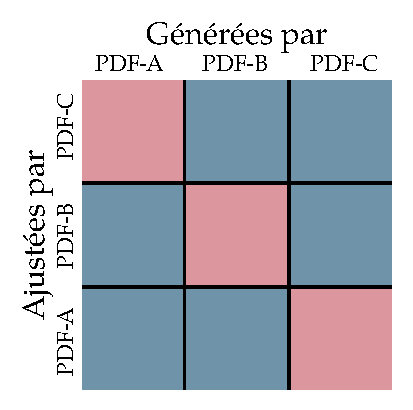
\includegraphics[width=0.48\textwidth]{chapitre7/figs/pull_matrix.pdf}
  \caption{Représentation schématique d'une matrice des \emph{pull}. Chaque colonne (ligne) correspond aux distributions de \emph{pull} obtenues sur des pseudo\-/expériences générées (ajustées) par une des trois fonctions. Les distributions sur la diagonale sont non-biaisées par définition, puisque la même fonction sert à la fois à la génération et à l'ajustement.}
  \label{fig:pull_matrix}
\end{figure}

\begin{figure}[tbp]
  \centering
  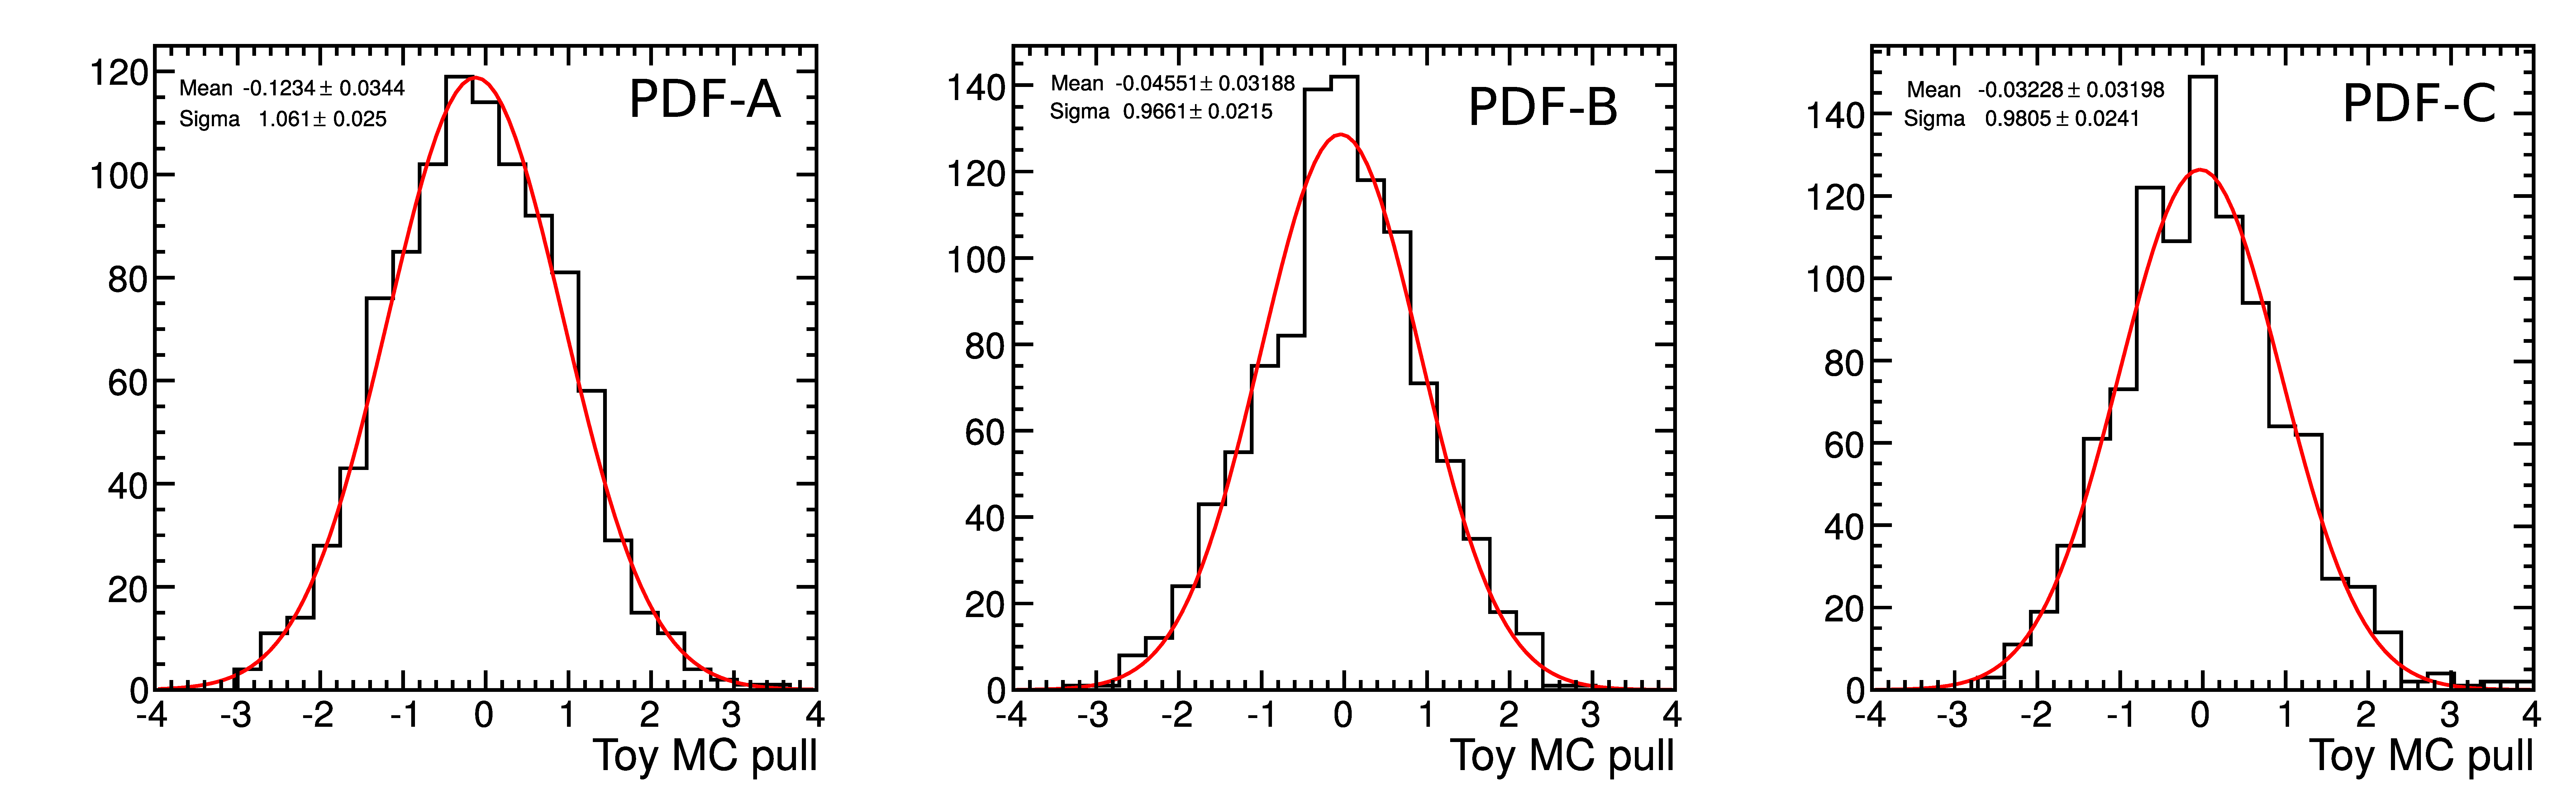
\includegraphics[width=\textwidth]{chapitre7/figs/alterfit_750.pdf}
  \caption{Distributions de \emph{pull} obtenues suite à l'ajustement des pseudo\-/expériences par \ref{pdfA} (gauche), \ref{pdfB} (centre), et \ref{pdfC} (droite). Les pseudo\-/expériences utilisées lors de l'ajustement par une fonction sont générées à l'aide des deux autres fonctions considérées.}
  \label{fig:pulls}
\end{figure}

Au final, on obtient 9 distributions de \emph{pull}, une pour chaque couple \enquote{fonction ayant générée les pseudo\-/expériences / fonction ayant ajustée les pseudo\-/expériences}. Une représentation schématique est visible sur la \cref{fig:pull_matrix}. On souhaite cependant obtenir un unique estimateur par fonction. On somme donc les distributions de \emph{pull} de chaque couple où la même fonction a servi à l'ajustement, en excluant le couple où la même fonction a servi à la génération et à l'ajustement, non biaisé. Autrement dit, si on se réfère à la \cref{fig:pull_matrix}, on somme les distributions associées à chaque ligne, en excluant la diagonale.

Les résultats de cette étude sont visibles \cref{fig:pulls} pour un \zprime de masse $\mzp = \SI{750}{\GeV}$, dans l'hypothèse de résonances étroites. Chaque distribution est ajustée avec une fonction gaussienne de laquelle on extrait la moyenne, décrivant le biais sur le nombre d'événement de signal de la fonction utilisée pour l'ajustement des pseudo\-/expériences.

\smallskip

On répète cette même procédure pour chaque point de masse. Les résultats sont consignés dans le \cref{tab:bias_mtt}. Pour chaque fonction, on regarde la valeur de la moyenne de la distribution de \emph{pull} liée à cette fonction. Parmi les trois fonctions, on constate que \ref{pdfB} minimise le biais sur le nombre d'événements de signal. C'est pour cette raison qu'il a été décidé d'utiliser \ref{pdfB} comme fonction analytique pour décrire le fond.

\begin{table}[htbp] \centering
  \sisetup{detect-weight = true}
  \begin{tabular}{@{}cccc@{}} \toprule

    \mzp & \ref{pdfA} & \ref{pdfB} & \ref{pdfC} \\ \midrule

    \SI{500}{\GeV} & \num{0.061 \pm 0.034} & \num{-0.045 \pm 0.033} & \num{-0.029 \pm 0.032} \\
    \SI{750}{\GeV} & \num{-0.12 \pm 0.03} & \num{-0.032 \pm 0.032} & \num{-0.046 \pm 0.032} \\
    \SI{1000}{\GeV} & \num{0.32 \pm 0.03} & \num{0.059 \pm 0.032} & \num{0.088 \pm 0.036} \\
    \SI{1250}{\GeV} & \num{- 0.17 \pm 0.03} & \num{0.090 \pm 0.037} & \textbf{0,37(3)} \\
    \SI{1500}{\GeV} & \textbf{−0,43(3)} & \textbf{0,21(4)} & \num{0.046 \pm 0.034} \\
    \bottomrule

  \end{tabular}
  \caption{Valeurs moyennes extraites des distributions de \emph{pull} par une interpolation gaussienne, pour chaque fonction considérée. Les valeurs en gras correspondent au biais le plus grand pour chaque fonction.}
  \label{tab:bias_mtt}
\end{table}

La même étude a aussi été menée sans ajouter de signal au moment de la génération des pseudo-expériences. Les conclusions obtenues sont identiques à celles obtenues ci-dessus.

\subsection{Extraction du nombre d'événements de signal}

On effectue un ajustement simultané dans les quatre catégories de l'analyse, en utilisant la méthode du maximum de vraisemblance décrite ci-dessus. Le résultat de cet ajustement est visible \cref{fig:likelihood_fit}, pour un \zprime de masse $\mzp = \SI{750}{\GeV}$, dans l'hypothèse de résonances étroites. On extrait de l'ajustement la valeur la plus probable du nombre d'événements de signal, pour chaque masse et chaque hypothèse de signal. On transforme ce nombre d'événements en section efficace, selon la relation \ref{eq:cross_section}. Les sections efficaces obtenues sont résumées dans les \cref{tab:cross_section_zprime,tab:cross_section_kk}. Les incertitudes présentées dans ces tableaux ne tiennent compte que des erreurs statistiques.

\begin{figure}[tbp] \centering
    \subcaptionbox{Canal semi-muonique, au moins 2 jets étiquetés \Pbottom.}[0.48\textwidth]{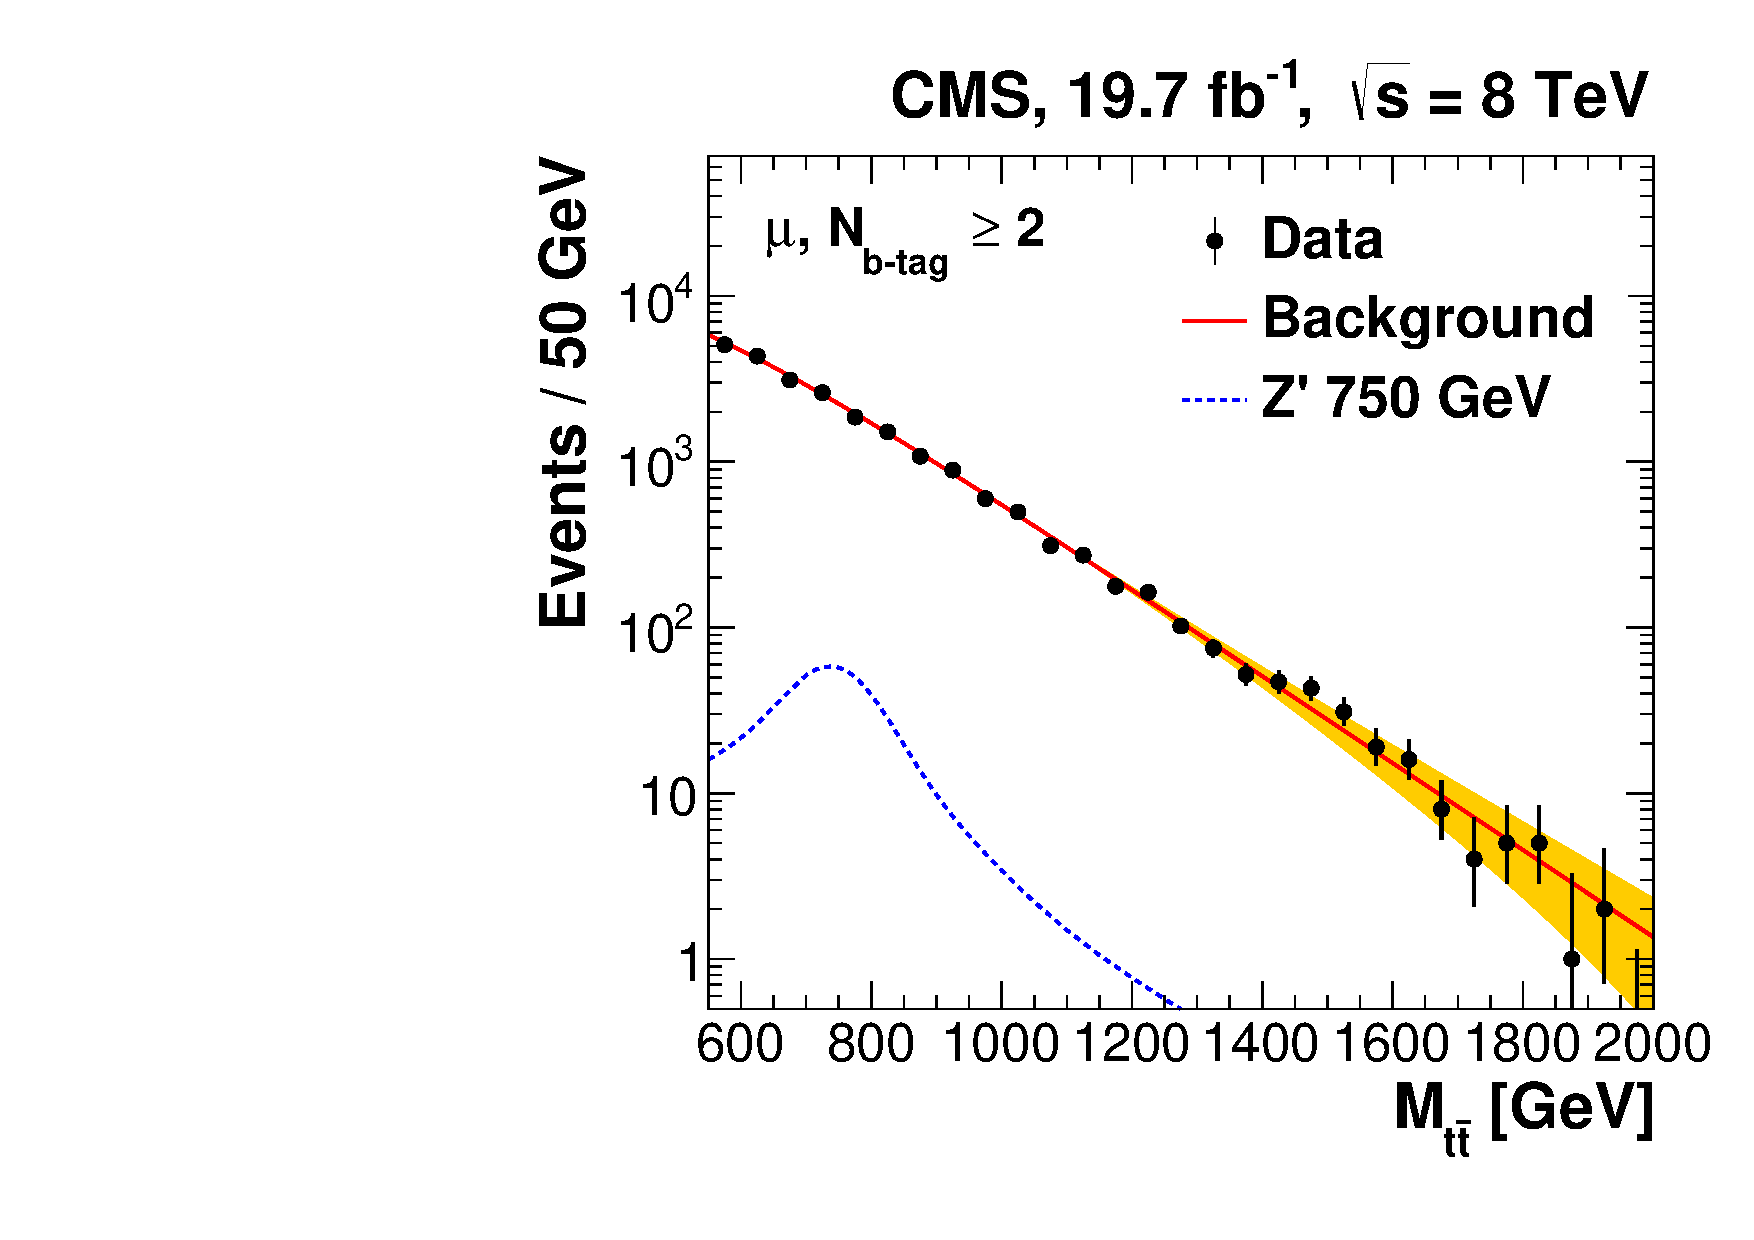
\includegraphics[width=0.48\textwidth,angle=-90,origin=c]{chapitre7/figs/likelihood_fit_mu_2b.pdf}} \hfill
    \subcaptionbox{Canal semi-électronique, au moins 2 jets étiquetés \Pbottom.}[0.48\textwidth]{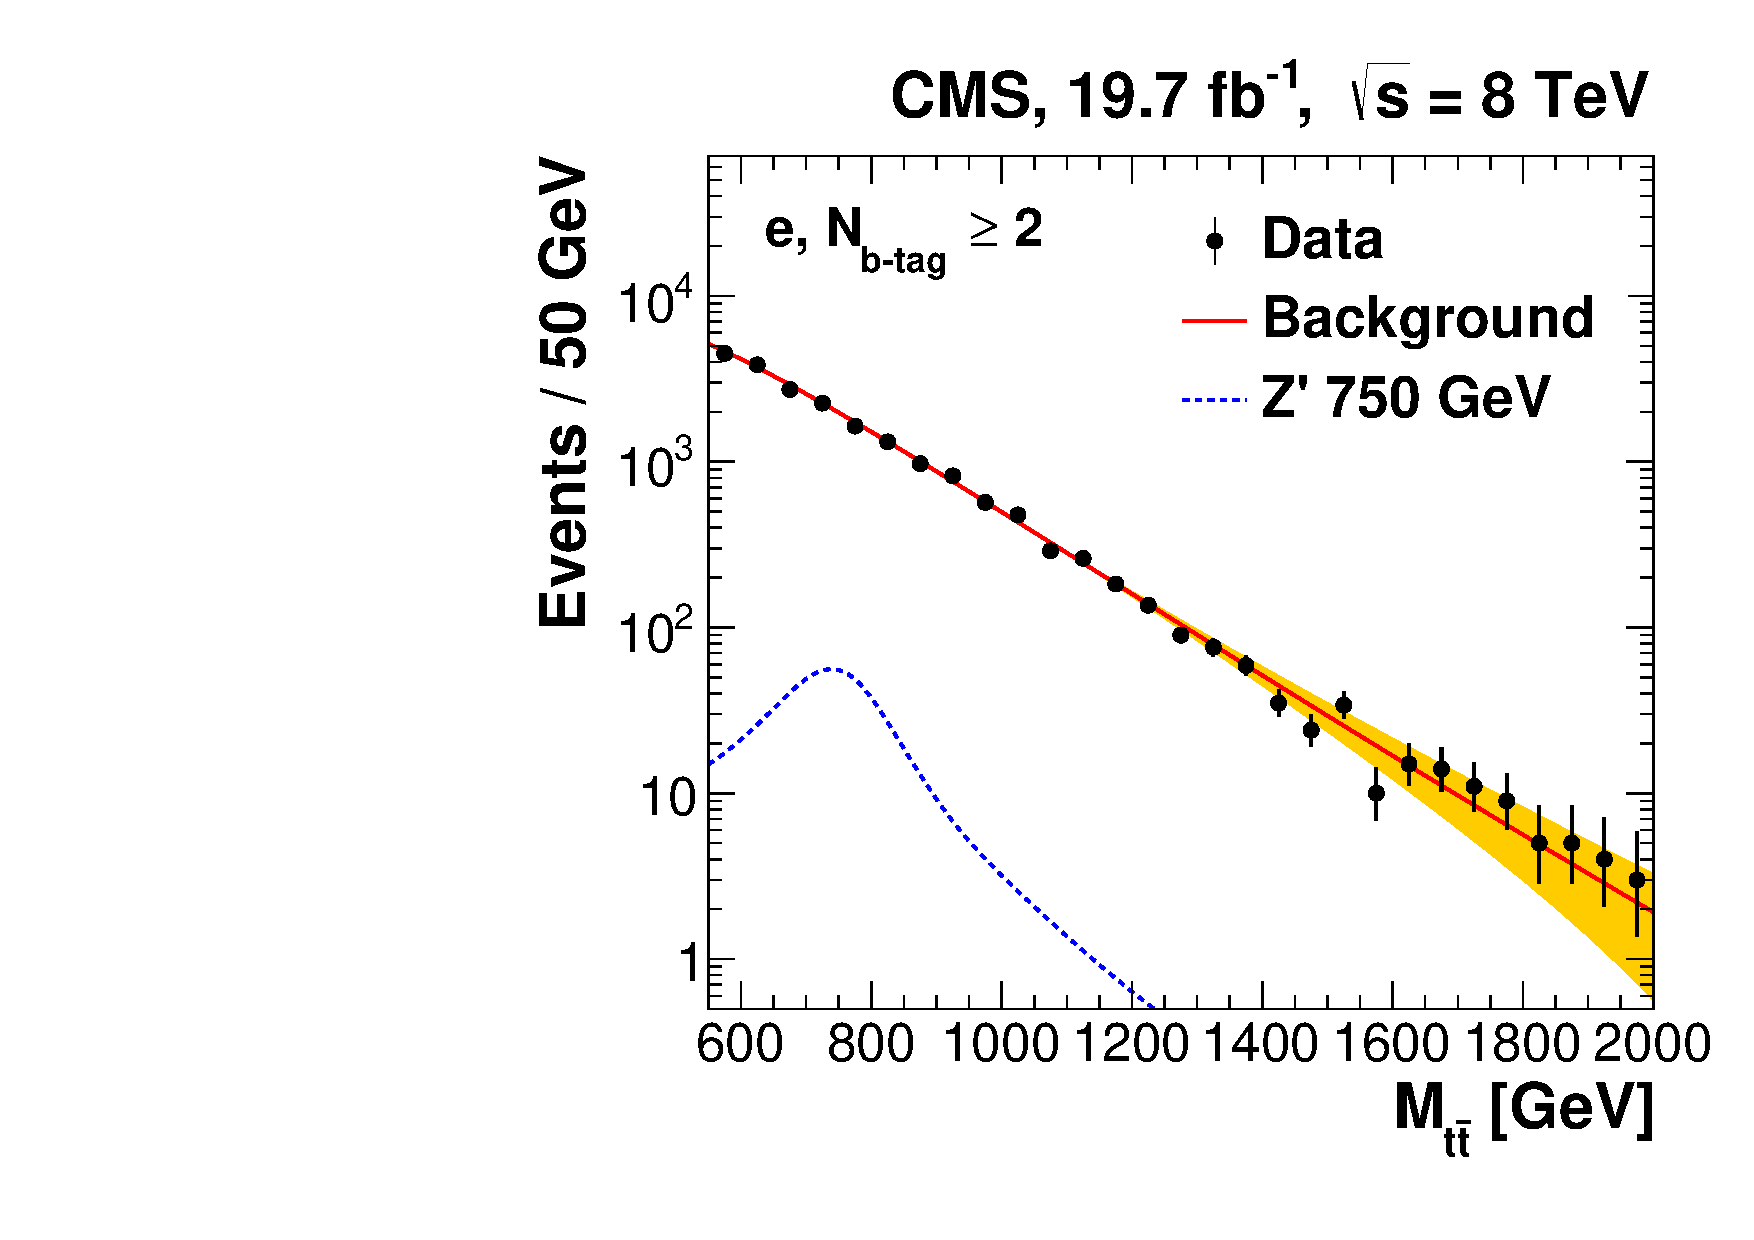
\includegraphics[width=0.48\textwidth,angle=-90,origin=c]{chapitre7/figs/likelihood_fit_e_2b.pdf}} \\
    \subcaptionbox{Canal semi-muonique, exactement 1 jet étiqueté \Pbottom.}[0.48\textwidth]{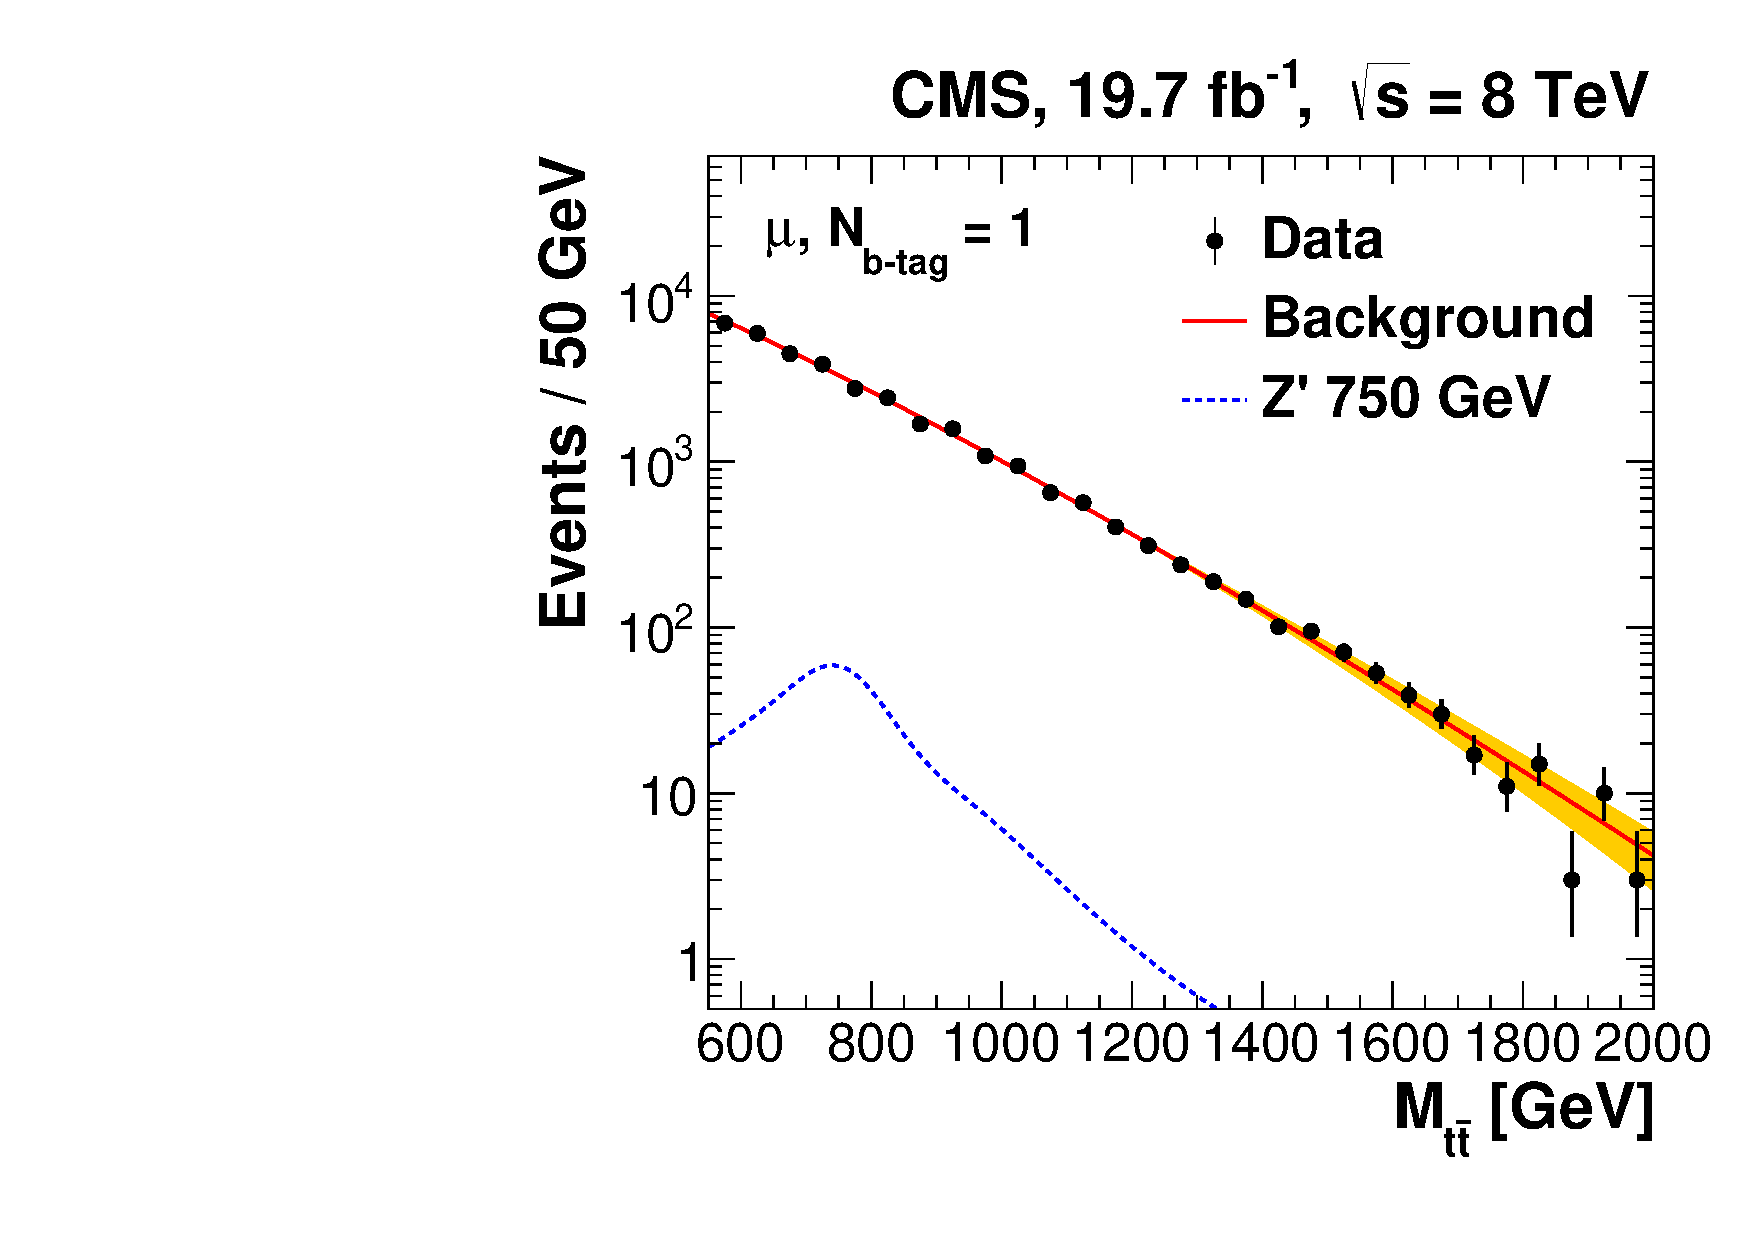
\includegraphics[width=0.48\textwidth,angle=-90,origin=c]{chapitre7/figs/likelihood_fit_mu_1b.pdf}} \hfill
    \subcaptionbox{Canal semi-électronique, exactement 1 jet étiqueté \Pbottom.}[0.48\textwidth]{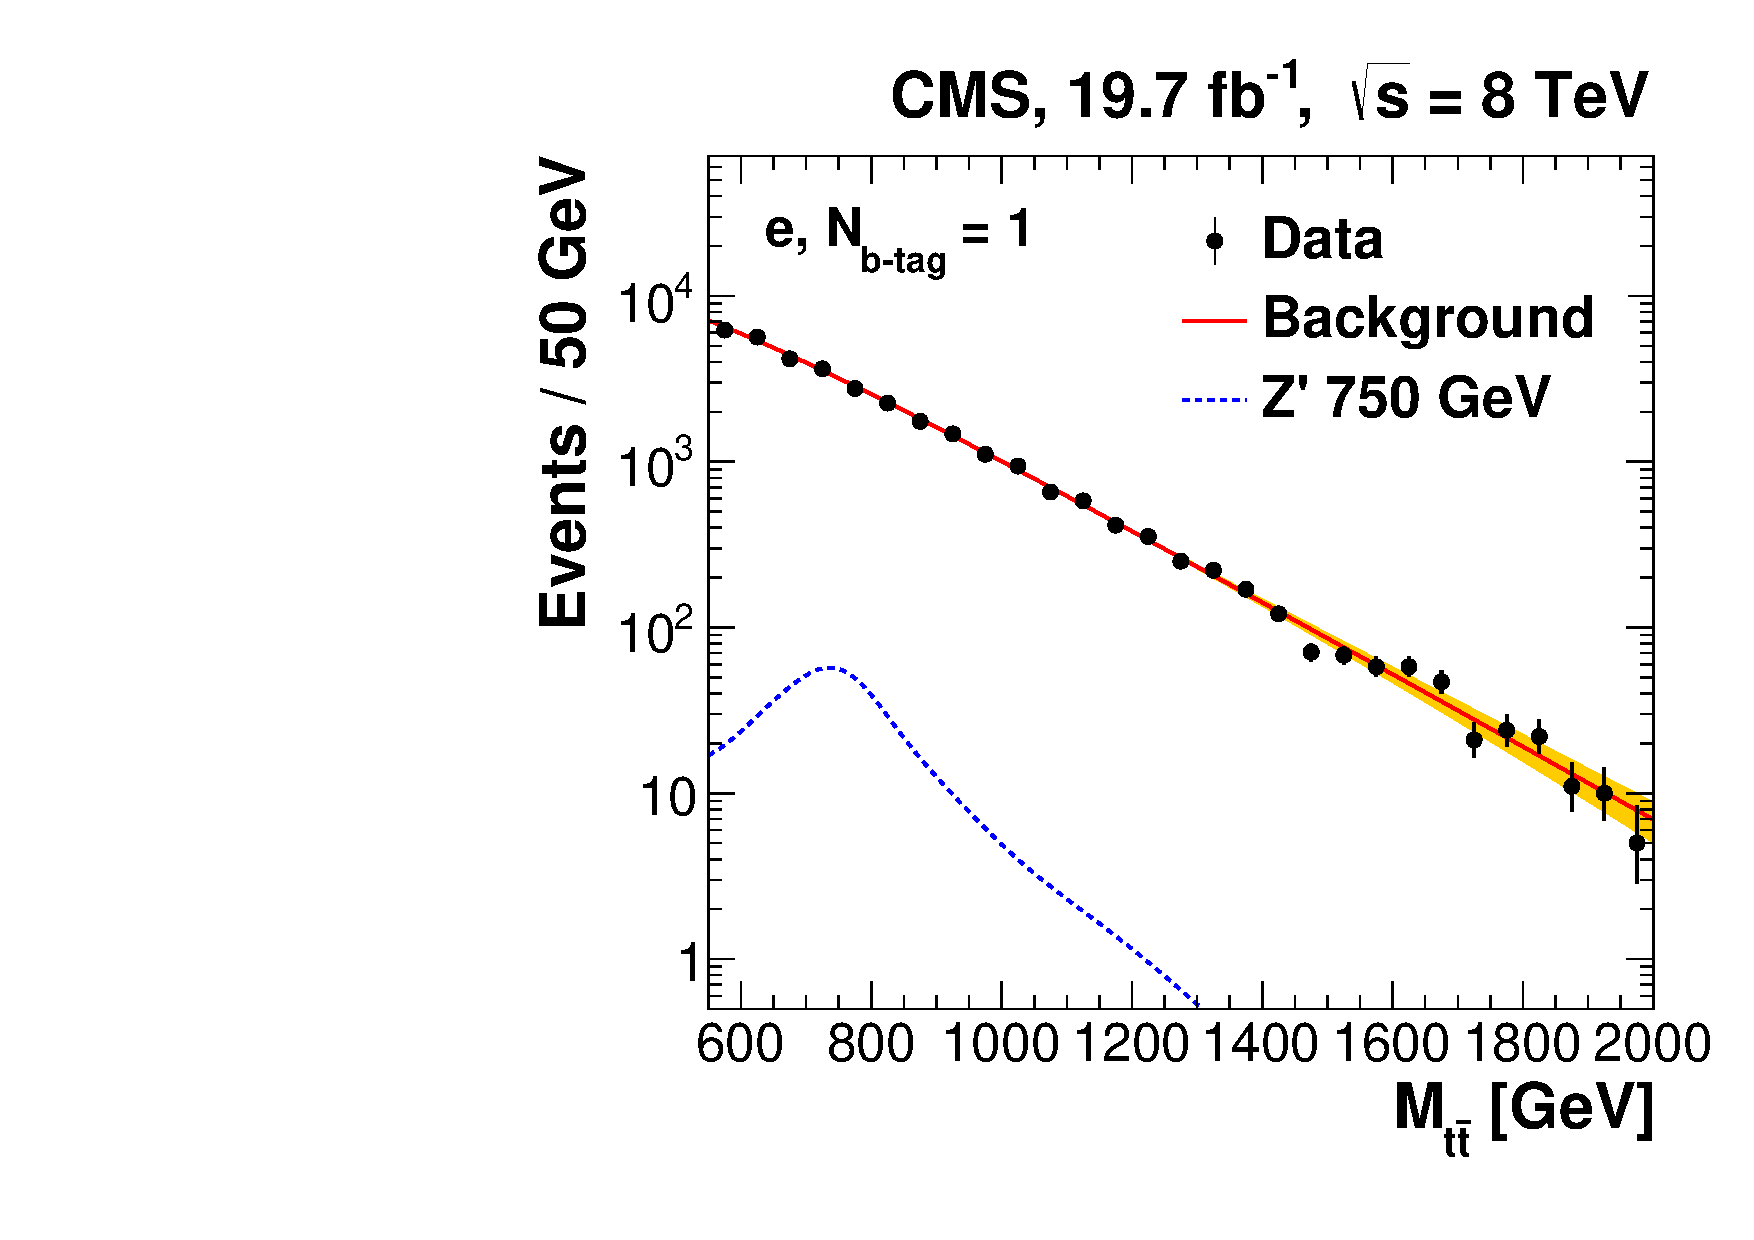
\includegraphics[width=0.48\textwidth,angle=-90,origin=c]{chapitre7/figs/likelihood_fit_e_1b.pdf}}
    \caption{Ajustement des données à l'aide de la méthode du maximum de vraisemblance en incluant un signal de masse $\mzp = \SI{750}{\GeV}$, dans l'hypothèse de résonances étroites, pour les 4 catégories de l'analyse. La bande jaune correspond à l'incertitude de l'ajustement, et la distribution du \zprime est normalisée à une section efficace de \SI{1}{\pb}.}
    \label{fig:likelihood_fit}
\end{figure}

\begin{table}[htbp] \centering

\begin{tabular}{@{}cccccc@{}} \toprule

 & \SI{500}{\GeV} & \SI{750}{\GeV} & \SI{1000}{\GeV} & \SI{1250}{\GeV} & \SI{1500}{\GeV} \\ \midrule
 $\sigma_{\zprime}$ (\si{\percent}) -- résonance étroite & \num{-0.11 \pm 0.87} & \num{-0.17 \pm 0.28} & \num{0.13 \pm 0.19} & \num{-0.14 \pm 0.18} & \num{0.05 \pm 0.16} \\
 $\sigma_{\zprime}$ (\si{\percent}) -- résonance large & \num{-0.00 \pm 0.79} & \num{-0.15 \pm 0.31} & \num{0.12 \pm 0.22} & \num{-0.15 \pm 0.23} & \num{0.00 \pm 0.2} \\ \bottomrule

\end{tabular}
\caption{Sections efficaces du signal extraites grâce à l'ajustement par la méthode du maximum de vraisemblance sur les données, dans le cas de \zprime. L'incertitude est purement statistique.}
\label{tab:cross_section_zprime}
\end{table}

\begin{table}[htbp] \centering

\begin{tabular}{@{}cccccc@{}} \toprule

 & \SI{500}{\GeV} & \SI{700}{\GeV} & \SI{1000}{\GeV} & \SI{1200}{\GeV} & \SI{1500}{\GeV} \\ \midrule
 $\sigma_{\kkglu}$ (\si{\percent}) & \num{-0.07 \pm 0.39} & \num{0.12 \pm 0.30} & \num{-0.04 \pm 0.29} & \num{0.12 \pm 0.30} & \num{-0.13 \pm 0.26} \\ \bottomrule
\end{tabular}
\caption{Sections efficaces du signal extraites grâce à l'ajustement par la méthode du maximum de vraisemblance sur les données, dans le cas de gluons de Kaluza-Klein. L'incertitude est purement statistique.}
\label{tab:cross_section_kk}
\end{table}

On constate que toutes les sections efficaces obtenues sont compatibles avec 0, c'est-à-dire une absence de signal. Néanmoins, cette absence ne signifie pas qu'aucun signal de nouvelle physique n'est présent, mais seulement que notre analyse n'est pas capable de le détecter. Afin de quantifier notre sensibilité en terme de section efficace, on utilise une méthode statistique, décrite dans la prochaine section.

\subsection{Extraction des limites}

On utilise une méthode bayésienne afin de quantifier la sensibilité de notre analyse. La fonction de vraisemblance peut être reliée à la densité de probabilité à posteriori (\emph{posterior}) $p(\sigma, \theta \mid \mtt)$, représentant la probabilité que les paramètres libres soient compatibles avec l'observation, par le théorème de Bayes :
\begin{align*}
  p(\sigma, \theta \mid \mtt) &= \frac{\mathcal{L}(\mtt \mid \sigma, \theta) \pi(\sigma) \pi(\theta)}{\int{\mathcal{L}(\mtt \mid \sigma^\prime, \theta^\prime) \pi(\sigma^\prime) \pi(\theta^\prime) \, \mathrm{d}\sigma^\prime \mathrm{d}\theta^\prime}}
\end{align*}
où $\theta$ symbolise l'ensemble des paramètres libres de l'ajustement (face à son importance, la section efficace $\sigma$ est considérée à part des autres paramètres), $\mathcal{L}(\mtt \mid \sigma, \theta)$ est la fonction de vraisemblance, et $\pi(\sigma, \theta)$ le \emph{prior}, une densité de probabilité qui représente notre connaissance des paramètres avant l'ajustement. On impose à la section efficace d'être positive
\begin{align*}
\pi(\sigma) = \begin{cases} \frac{1}{\sigma_\text{max} - \sigma_\text{min}} &\mbox{si } \sigma \geq 0 \\
0 & \mbox{si } \sigma < 0 \end{cases}
\end{align*}
et on assigne aux autres paramètres un \emph{prior} plat ($\pi(\theta) = \frac{1}{\theta_\text{max} - \theta_\text{min}}$). Les valeurs "min" et "max" représentent l'intervalle des valeurs autorisées pour les \emph{prior}.

\medskip

Des erreurs systématiques, inhérentes aux techniques expérimentales, modifient la mesure de la section efficace. Pour chaque erreur systématique (ou paramètre de nuisance), on ajoute au calcul du \emph{posterior} un \emph{prior}, qui permet de décrire notre connaissance limitée des différentes étapes de la reconstruction. Si l'on symbolise par $\nu$ l'ensemble des paramètres de nuisances, le \emph{posterior} s'écrit maintenant :
\begin{align*}
  p(\sigma, \theta, \nu \mid \mtt) &= \frac{\mathcal{L}(\mtt \mid \sigma, \theta) \pi(\sigma) \pi(\theta) \pi(\nu)}{\int{\mathcal{L}(\mtt \mid \sigma^\prime, \theta^\prime) \pi(\sigma^\prime) \pi(\theta^\prime) \pi(\nu^\prime) \, \mathrm{d}\sigma^\prime \mathrm{d}\theta^\prime \mathrm{d}\nu^\prime}}
\end{align*}

On utilise comme \emph{prior} une gaussienne centrée autour de la valeur la plus probable du paramètre de nuisance, et d'écart-type l'incertitude sur ce paramètre. Dans le cas où le paramètre ne peut pas être négatif (comme une efficacité), on préfère utiliser une fonction log-normal au lieu d'une gaussienne tronquée à zéro. Le \emph{prior} log-normal est défini par
\begin{align*}
  \pi(\nu) &= \frac{1}{\nu \sigma \sqrt{2} \pi} \exp{\left( - \frac{\left( \ln\nu - \hat{\nu}\right)^2}{2 \sigma^2} \right)}
\end{align*}

Cependant, le seul paramètre d'intérêt est la section efficace du signal. On intègre alors tous les paramètres de nuisance du \emph{posterior} afin de ne garder que la dépendance à la section efficace. On considère les paramètres libres des PDFs du signal et du fond comme des paramètres de nuisance. On a alors
\begin{align*}
  p(\sigma \mid \mtt) &= \iint{ p(\sigma, \theta, \nu \mid \mtt) \; \mathrm{d\theta} \, \mathrm{d} \nu }
\end{align*}

Le nombre de dimensions de l'intégrale est souvent trop important pour qu'elle soit calculable analytiquement. On utilise à la place une méthode d'intégration numérique, basée sur une méthode Monte-Carlo par chaîne de Markov (MCMC) \citep{metropolis,hastings70}.

\smallskip

Le \emph{posterior} peut également être utilisé afin d'établir un intervalle de confiance. Il est ainsi possible de définir une limite supérieure $\sigma_\text{up}$ sur la section efficace à un certain niveau de confiance $1 - \alpha$ (habituellement \SI{95}{\percent}) : en refaisant l'expérience plusieurs fois, la probabilité d'obtenir une section efficace supérieure à $\sigma_\text{up}$ est égale $ \alpha$.
La limite supérieure est définie comme la borne supérieur de l'intégrale :
\begin{align*}
  1 - \alpha = \int \limits_{-\infty}^{\sigma_{\text{up}}} p(\sigma \mid \mtt) \; \mathrm{d} \sigma
\end{align*}

\subsubsection{Erreurs systématiques}

Des erreurs systématiques peuvent modifier la mesure de la section efficace, en affectant l'efficacité de sélection ou le nombre d'événements de signal attendu. Toutes ces erreurs sont considérées comme des paramètres de nuisances et sont introduites dans le calcul du \emph{posterior} en utilisant des \emph{prior} log-normal. Les sources suivantes d'incertitudes systématiques sont considérées dans l'analyse :

\begin{table}[p] \centering
  \begin{tabular}{@{}ccccc@{}} \toprule
  Erreur & semi-$\mu$, 1 \Pbottom & semi-e, 1 \Pbottom & semi-$\mu$, 2 \Pbottom & semi-e, 2 \Pbottom \\ \midrule
  Luminosité & \SI{4.4}{\percent} & \SI{4.4}{\percent} & \SI{4.4}{\percent} & \SI{4.4}{\percent} \\
  JEC & \SI{1.08}{\percent} & \SI{1.08}{\percent} & \SI{1.08}{\percent} & \SI{1.08}{\percent} \\
  JER & \SI{0.07}{\percent} & \SI{0.07}{\percent} & \SI{0.07}{\percent} & \SI{0.07}{\percent} \\
  Repondération du \pu & \SI{0.05}{\percent} & \SI{0.05}{\percent} & \SI{0.05}{\percent} & \SI{0.05}{\percent} \\
  PDF du signal & \SI{0.64}{\percent} & \SI{0.64}{\percent} & \SI{0.64}{\percent} & \SI{0.64}{\percent} \\
  Efficacité & \SI{3.45}{\percent} & \SI{3.42}{\percent} & \SI{4.03}{\percent} & \SI{4.01}{\percent} \\
  \bottomrule
  \end{tabular}
  \caption{Erreurs systématiques introduites dans le calcul du \emph{posterior}, pour un \zprime de masse $\mzp = \SI{750}{\GeV}$, dans l'hypothèse de résonances étroites.}
  \label{tab:syst}
\end{table}

\begin{figure}[p]
  \centering
  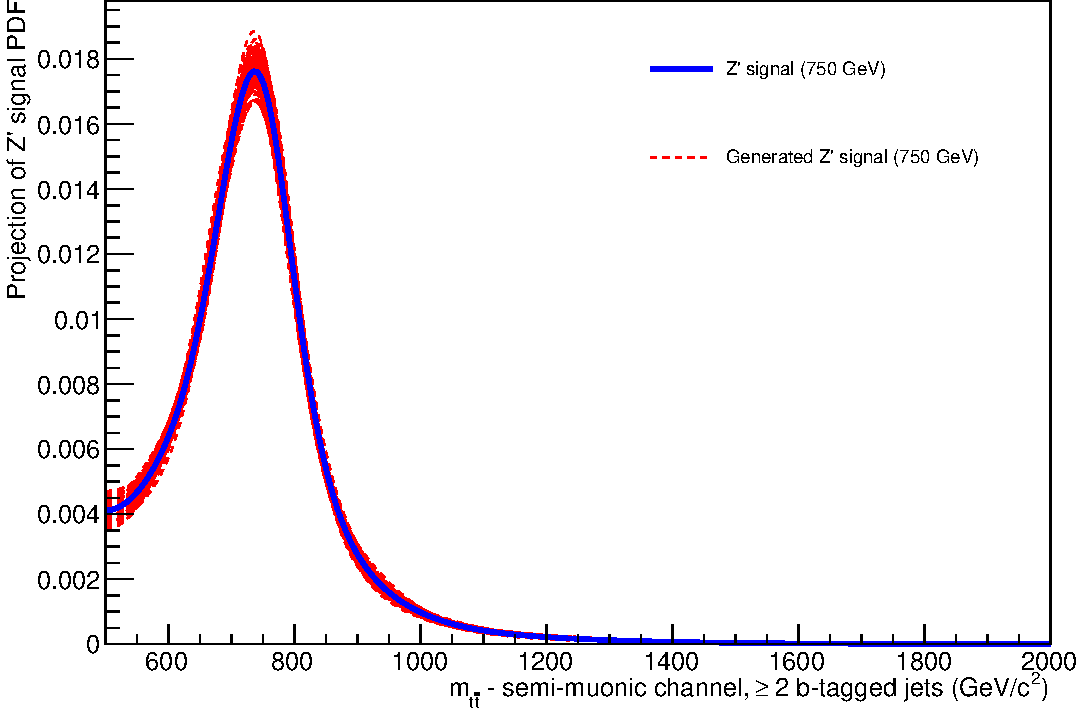
\includegraphics[width=0.8\textwidth]{chapitre7/figs/keyspdf_overlaid_750_2_btag_muon.pdf}
  \caption{PDFs du signal utilisées pour calculer l'erreur systématique sur le choix de la PDF de signal pour un \zprime de masse $\mzp = \SI{750}{\GeV}$, dans l'hypothèse de résonances étroites. La PDF nominale est en bleue, et les 150 PDFs générées à partir des pseudo\-/expériences sont en rouge.}
  \label{fig:keys_syst}
\end{figure}

\begin{description}
  \item[Luminosité] L'incertitude sur la mesure de la luminosité (\SI{4.4}{\percent}) est considérée comme une source d'erreur systématique.
  \item[\pu] La section efficace des collisions \Pproton{}\Pproton{} utilisée lors du calcul des facteurs de repondération du \pu est variée de \pm{} \SI{5}{\percent}. La variation de la section efficace du signal extraite est considérée en tant qu'erreur systématique.
  \item[Facteurs de corrections] Les incertitudes sur les facteurs de corrections liés à l’identification et à l’isolation des leptons, à l’algorithme d’étiquetage des jets de b ainsi qu’aux performances des chemins de déclenchement sont sommées en quadratique et considérées comme une source d’incertitude systématique impactant l'efficacité de la sélection.
  \item[Corrections des jets] Les incertitudes sur les corrections en énergie et résolution des jets sont considérées comme une source d’incertitude systématique. Afin d'en tenir compte, les facteurs de corrections des jets sont modifiés de \pm{} leur incertitude, et l'analyse complète est refaite. La variation de la section efficace du signal extraite à l'aide de l'ajustement est considérée comme incertitude systématique.
  \item[Modélisation du signal] On utilise une interpolation par noyaux gaussiens pour décrire la PDF du signal, déterminée sur des événements de signal simulés. Cette PDF est fixée pendant l'ajustement. Afin d'évaluer l'effet systématique du choix de cette description du signal sur $N_S$, on génère environ 150 pseudo\-/expériences pour chaque point de masse à partir de l'interpolation du signal. Pour chaque pseudo\-/expérience, on extrait une nouvelle PDF pour le signal (voir \cref{fig:keys_syst}), qu'on utilise pour extraire une nouvelle valeur de $N_S$. On obtient ainsi une distribution de $N_S$, dont on utilise la moyenne quadratique (RMS) comme erreur systématique liée au choix de PDF du signal.
  \item[Densités de probabilité partonique] Les fonctions de densité de probabilité partonique ne sont connues qu'avec une certaine précision. Les valeurs propres de ces fonctions sont modifiées dans leurs incertitudes lors la simulation du signal, et l'analyse est refaite avec la nouvelle fonction de densité partonique. L'effet sur le nombre d'événements de signal est négligeable par rapport aux autres erreurs systématiques, et n'est pas inclus dans la liste des incertitudes systématiques.
\end{description}

À titre d'exemple, le \cref{tab:syst} résume les valeurs des erreurs systématiques pour un \zprime de masse $\mzp = \SI{750}{\GeV}$, dans l'hypothèse de résonances étroites.

\section{Résultats}

\begin{figure}[p!]
  \centering
  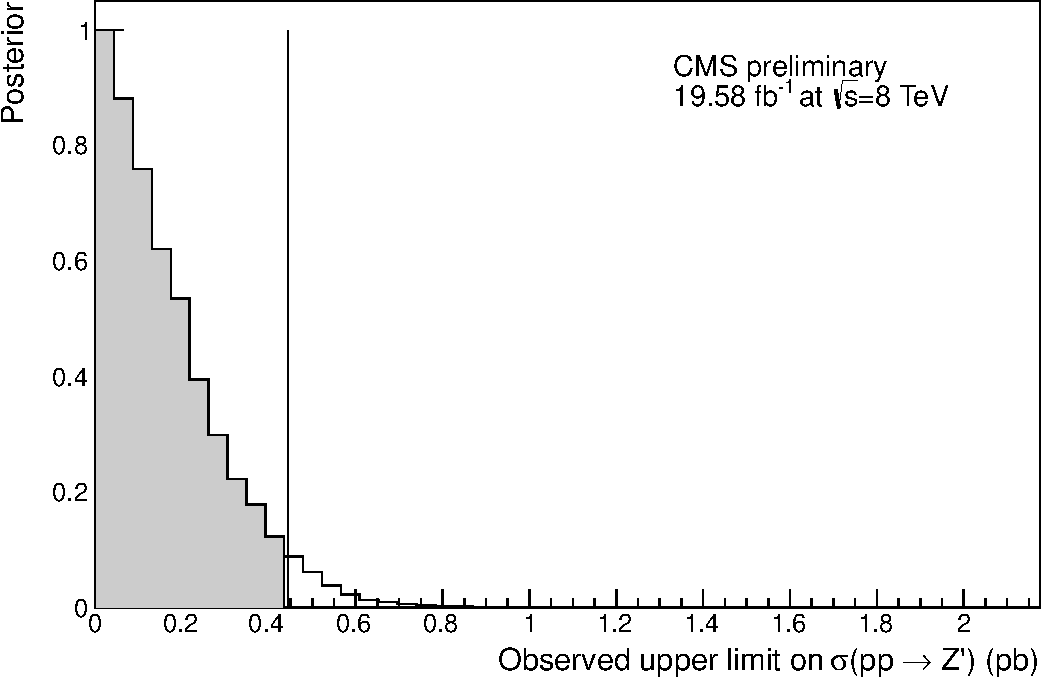
\includegraphics[width=0.7\textwidth]{chapitre7/figs/posterior_plot_750.pdf}
  \caption{Distribution du \emph{posterior} $p(\sigma \mid \mtt)$ obtenue grâce à une intégration numérique par méthode MCMC sur les données, pour un \zprime de masse $\mzp = \SI{750}{\GeV}$, dans l'hypothèse de résonances étroites. La zone en grise correspond au \SI{95}{\percent} de la distribution, utilisée pour extraire la limite supérieure sur la section efficace (ligne verticale).}
  \label{fig:posterior}
\end{figure}

\begin{figure}[p!]
  \centering
  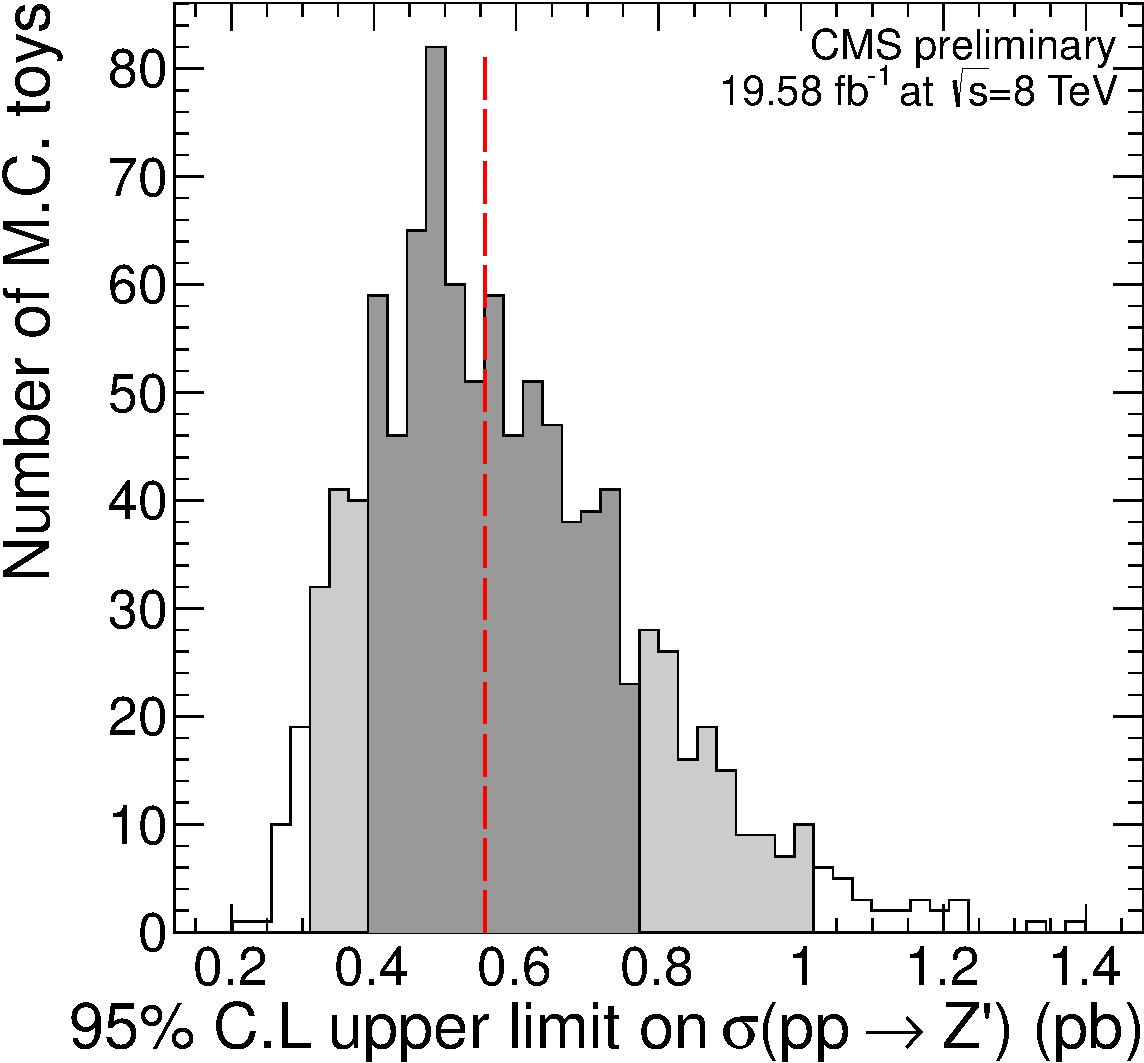
\includegraphics[width=0.7\textwidth]{chapitre7/figs/posterior_plot_expected_750.pdf}
  \caption{Distribution des limites supérieures extraites obtenus sur environ 500 pseudo\-/expériences. La ligne rouge correspond à la limite attendue, médiane de la distribution. Les zones en gris foncé et gris clair correspondent respectivement aux intervalles de confiance à 68 et \SI{95}{\%} sur la limite attendue.}
  \label{fig:posterior_mc}
\end{figure}

Afin de quantifier la sensibilité de notre analyse, on calcule la limite supérieure sur la section efficace pour un niveau de confiance de \SI{95}{\percent} pour chaque point de masse et chaque type de signal.
On cherche à calculer deux types de quantités :
\begin{itemize}
  \item Les limites observées, extraites en utilisant les données. Pour chaque point de masse, on calcule la limite supérieure à \SI{95}{\percent} en utilisant la méthode décrite ci-dessus. Le \emph{posterior} obtenu pour un \zprime de masse $\mzp = \SI{750}{\GeV}$, dans l'hypothèse de résonances étroites, est représenté sur la \cref{fig:posterior}. Cette distribution est intégrée afin d'extraire la limite supérieure.
  \item Les limites attendues, extraites de façon similaire aux limites observées, mais en utilisant des pseudo\-/expériences générées à l'aide de la PDF de fond au lieu des données, c'est-à-dire sans aucun signal. On extrait la limite supérieure sur environ \num{500} pseudo\-/expériences, pour obtenir une distribution des limites supérieures. De cette distribution, on extrait la valeur nominale, définie par la médiane de la distribution, ainsi qu'un intervalle de confiance de \SI{68}{\percent} et \SI{95}{\%} en intégrant 68 ou \SI{95}{\percent} de la distribution autour de la médiane. Un exemple de distribution est visible sur la \cref{fig:posterior_mc} pour un \zprime de masse $\mzp = \SI{750}{\GeV}$, dans l'hypothèse de résonances étroites.
\end{itemize}

\begin{figure}[tbp] \centering
    \subcaptionbox{Hypothèse de résonances étroites.}[0.8\textwidth]{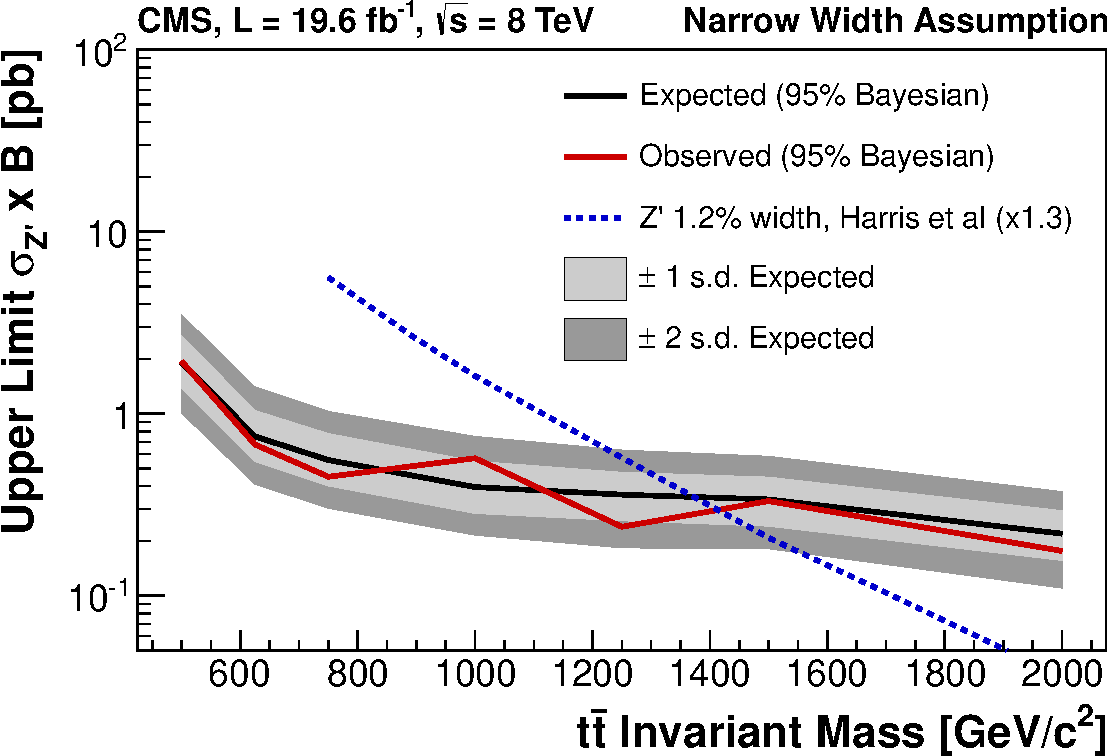
\includegraphics[width=0.8\textwidth]{chapitre7/figs/limits_narrow.pdf}} \\ \vspace{5mm}
    \subcaptionbox{Hypothèse de résonances larges.}[0.8\textwidth]{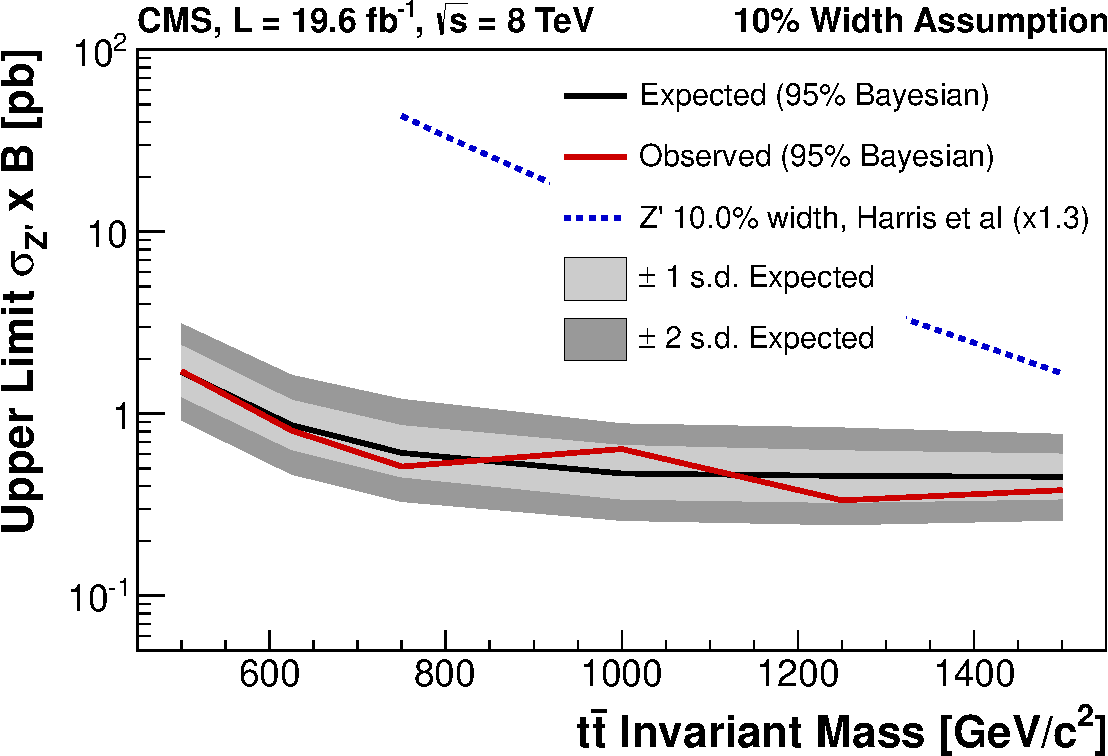
\includegraphics[width=0.8\textwidth]{chapitre7/figs/limits_large.pdf}}
    \caption{Courbes de limites pour des \zprime. La ligne rouge correspond aux limites observées, la ligne noire aux limites attendues, la bande gris clair à l'intervalle de confiance à \SI{68}{\percent} et la bande gris foncé à l'intervalle de confiance à \SI{95}{\%}. La ligne bleue correspond aux prédictions théorique pour un \zprime topcolor leptophobique \citep{Harris:2011ez}, multipliées par un facteur \num{1.3} pour obtenir une section efficace aux ordres supérieurs..}
    \label{fig:limits_zprime}
\end{figure}

On compare ensuite les limites attendues et observées sur les \cref{fig:limits_zprime,fig:limits_kk}. Les limites observées vont fluctuer autour des limites attendues, et un désaccord entre ces limites de plus de 2$\sigma$ (la limite observée est en dehors de l'intervalle de confiance à \SI{95}{\%}) serait le signe d'une déviation dans les données qui s'éloigne des prédictions du Modèle Standard\footnote{Il est a noter que dans ce cas, l'étape précédente d'extraction du nombre d'événements de signal aurait mis en évidence un excès d'événements par rapport à la prédiction théorique.}, soit le signe d'un problème de modélisation du fond ou du signal par l'analyse. Comme on peut le voir sur les courbes de limites, la limite supérieure sur la section efficace du signal est pleinement compatible avec l'hypothèse d'absence de signal.

\begin{figure}[tbp] \centering
    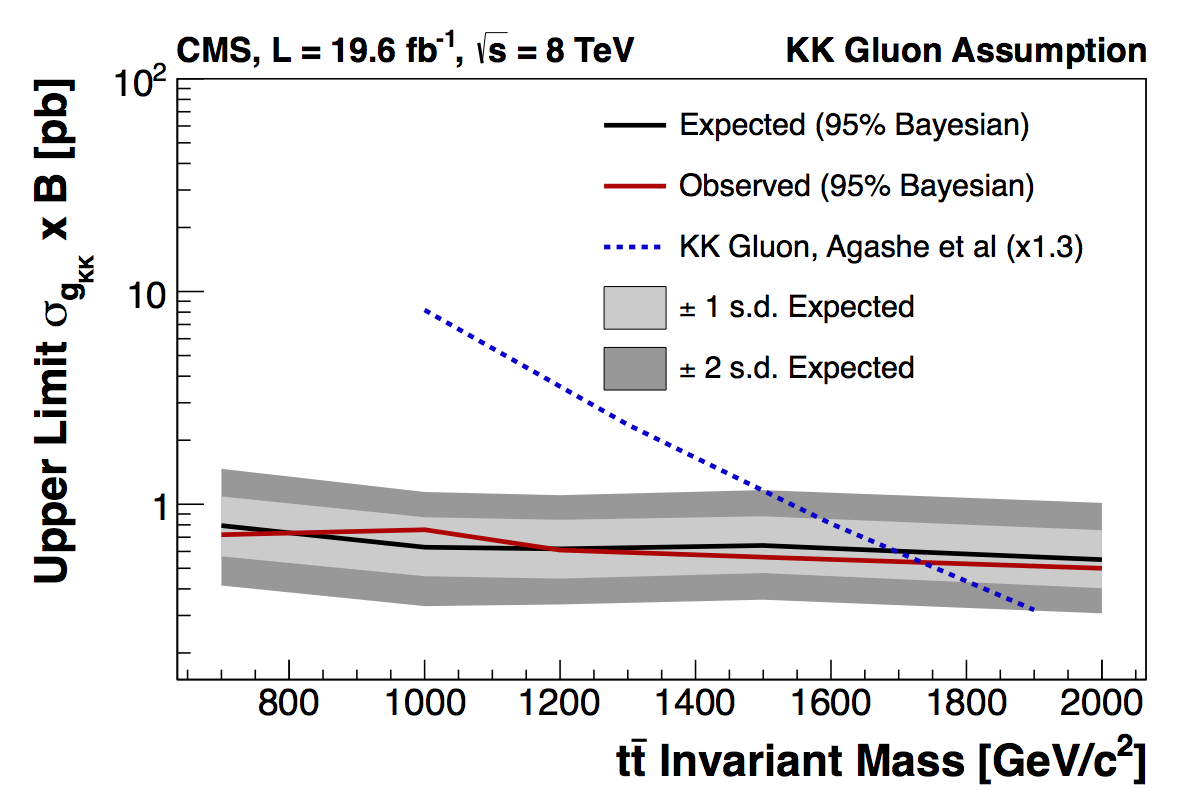
\includegraphics[width=0.8\textwidth]{chapitre7/figs/low-mass-limits-kk.png}
    \caption{Courbes de limites pour des gluons de Kaluza-Klein. La ligne rouge correspond aux limites observées, la ligne noire aux limites attendues, la bande gris clair à l'intervalle de confiance à \SI{68}{\percent} et la bande gris foncé à l'intervalle de confiance à \SI{95}{\%}. La ligne bleue correspond aux prédictions théorique pour ds gluons de Kaluza-Klein dans le modèle Randall-Sundrum \citep{Agashe:2006hk}, multipliées par un facteur \num{1.3} pour obtenir une section efficace aux ordres supérieurs.}
    \label{fig:limits_kk}
\end{figure}

\medskip

On superpose en plus sur les courbes de limites les prédictions théoriques de certains modèles particuliers. On considère dans le cas du \zprime un modèle topcolor, où le \zprime est leptophobique \citep{Harris:2011ez}, et pour les gluons de Kaluza-Klein, le modèle de Randall-Sundrum \citep{Agashe:2006hk}, utilisé pour la génération du signal. En comparant les limites observées et les prédictions théoriques, il est possible d'exclure certaines masses de résonances. En effet, si la prédiction théorique est plus grande que la limite observée, cela signifie que notre analyse est assez sensible pour détecter des résonances dans le spectre de masse \ttbar ayant cette section efficace. Le fait que rien ne soit observé permet ainsi d'exclure certaines masses pour un modèle particulier. Les exclusions réalisées par notre analyse sont résumées dans le tableau \cref{tab:limits}.

\begin{table}[htbp] \centering
  \begin{tabular}{@{}cc@{}} \toprule
    Modèle & Exclusion \\ \midrule
    \zprime, hypothèse de résonances étroites & $< \SI{1.4}{\TeV}$ \\
    \zprime, hypothèse de résonances larges & jusqu'à \SI{1.5}{\TeV} \\
    Gluons de Kaluza-Klein & $ < \SI{1.7}{\TeV}$ \\ \bottomrule
  \end{tabular}
  \caption{Gamme de masses exclues par l'analyse pour les différents modèles considérés.}
  \label{tab:limits}
\end{table}

\section{Combinaison et état de l'art}

L'analyse présentée dans ce chapitre est optimisée pour les résonances non boostées, correspondant à une masse inférieure à \tilde\SI{1}{\TeV}. Afin d'être efficace même à haute masse, cette analyse est combinée avec une autre, cette fois ci optimisée pour les résonances boostées \citep{CMS:lhr}, afin d'obtenir les limites les plus basses possibles sur toute la gamme de masse considérée. Dans cette analyse, le lepton n'est plus nécessairement isolé, et il est nécessaire d'avoir au moins deux jets, dont un d'au moins \SI{170}{\GeV}. En effet, on s'attend dans ces régimes à ce que les jets provenant de la désintégration du \PW hadronique soient agglomérés au sein du même jet, et dans des cas encore plus boostés, à ce que tous les jets provenant de la désintégration du quark top hadronique soient agglomérés au sein du même jet. Il est donc nécessaire de relâcher la contrainte sur le nombre de jet sélectionné pour reconstruire efficacement ces événements.

\medskip

\begin{figure}[p]
  \centering
  \includegraphics[width=0.80\textwidth]{chapitre7/figs/limits_narrow_combined.pdf}
  \caption{Courbe d'exclusion pour des \zprime, dans l'hypothèse de résonances étroites, obtenue en combinant notre analyse et l'analyse boostée. La légende est décrite en détails dans la légende de la \cref{fig:limits_zprime}. La ligne verticale correspond au point de transition entre les limites de notre analyse et celles de l'analyse boostée.}
  \label{fig:limits_narrow_cms}
\end{figure}

\begin{figure}[p]
  \centering
  \includegraphics[width=0.80\textwidth]{chapitre7/figs/limits_narrow_full_comb.pdf}
  \caption{Courbe d'exclusion pour des \zprime, dans l'hypothèse de résonances étroites, obtenue en combinant les analyses semi-leptonique et tout-hadronique. La légende est décrite en détails dans la légende de la \cref{fig:limits_zprime}. La ligne verticale correspond au point de transition entre les limites de notre analyse et celles des analyses boostées.}
  \label{fig:limits_narrow_cms_full}
\end{figure}

Il n'est pas possible d'effectuer une combinaison statistique entre ces deux analyses, puisque les sélections utilisées ne sont pas mutuellement exclusives (un même événement peut être sélectionné par les deux analyses). À la place, on utilise les limites de chaque analyse pour construire la courbe d'exclusion, et la transition entre les limites de cette analyse et celles de l'analyse boostée se fait en fonction de la sensibilité de la limite attendue. La \cref{fig:limits_narrow_cms} présente la courbe de limite ainsi obtenue pour des \zprime, dans l'hypothèse de résonances étroites : la ligne verticale correspond au point de transition entre les limites de cette analyse et celles de l'analyse boostée.

Une seconde combinaison est réalisée entre la première combinaison des analyses semi-leptonique et l'analyse exploitant le canal tout-hadronique, optimisée elle aussi pour les résonances boostées \citep{Chatrchyan:1599045}. Le résultat de cette combinaison est visible sur la \cref{fig:limits_narrow_cms_full}.

Il est intéressant de noter que, même si les analyses boostées sont meilleures à haute masse, l'analyse présentée dans ce chapitre reste indispensable à basse masse. On peut voir sur la \cref{fig:limits_comp} la comparaison entre les limites des trois analyses. Le gain apporté à basse masse par l'analyse est considérable, permettant de gagner jusqu'à un facteur 10 comparé à l'analyse boostée semi-leptonique.

\begin{figure}[tbp]
  \centering
  \includegraphics[width=0.6\textwidth]{chapitre7/figs/limit_comparison_narrow_resonances.pdf}
  \caption{Comparaison entre les limites de notre analyse (bleu), de l'analyse boostée semi-leptonique (rouge) et de l'analyse boostée tout-hadronique (orange). La courbe noire représente la limite obtenue après combinaison des trois analyses.}
  \label{fig:limits_comp}
\end{figure}

\bigskip

Le même type de recherche a aussi été mené au Tevatron par les expérience CDF et \dzero \citep{Aaltonen:2012af,Abazov:2011gv}. Ces analyses ne considèrent que le cas d'un \zprime étroit. Plus récemment, ATLAS a aussi publiée des résultats sur la recherche de résonances de spin 1 dans le spectre de masse \ttbar \citep{ATLAS-CONF-2013-052}. Il est à noter qu'ATLAS ne considère pas le cas de résonance large, et que l'analyse n'a pas encore été mise-à-jour avec toute la luminosité collectée par l'expérience : les comparaisons entre ATLAS et CMS ne sont donc pas réellement possibles. Le \cref{tab:comp_limits} résume les exclusions posées par les expériences ATLAS, CDF, CMS et \dzero, pour différents types de résonances de spin~1.

\begin{savenotes}
\begin{table}[ht] \centering
  \begin{tabular}{@{}ccccc@{}} \toprule
    Modèle & ATLAS\footnote{Seulement \SI{14.2}{\invfb} sur les \SI{20}{\invfb} disponibles ont été analysés par ATLAS} & CDF & CMS\footnote{Combinaison entre les analyses semi-leptoniques et tout-hadronique} & \dzero \\ \midrule
    \zprime, résonances étroites & \SI{1.8}{\TeV} & \SI{915}{\GeV} & \SI{2.1}{\TeV} & \SI{835}{\GeV} \\
    \zprime, résonances larges & - & - & \SI{2.7}{\TeV} & - \\
    Gluons de Kaluza-Klein & \SI{2.0}{\TeV} \footnote{Contrairement à CMS, le facteur \num{1.3} n'est pas inclut pour obtenir une section efficace théorique aux ordres supérieurs.} & - & \SI{2.5}{\TeV} & - \\
    \bottomrule
  \end{tabular}
  \caption{Exclusions posées par ATLAS, CDF, CMS et \dzero, pour différents types de résonances de spin 1.}
  \label{tab:comp_limits}
\end{table}
\end{savenotes}

\section{Conclusion}

Les résultats de la recherche de résonances de spin 1 dans le spectre de masse \ttbar ont été présentés tout au long de ce chapitre. Ces résultats, validés par la collaboration, ont été publiés au sein de la revue \emph{Physical Review Letters} \citep{Chatrchyan:1599045}, signe du grand intérêt porté par la communauté scientifique dans la recherche de nouvelle physique dans le secteur du quark top. La combinaison avec les analyses boostées semi- et tout-hadroniques permet d'obtenir les limites d'exclusions les plus hautes jamais posées sur la recherche de résonances de spin 1 se désintégrant en \ttbar à ce jour. Les \zprime leptophobiques dans le modèle topcolor sont exclus pour des masses inférieures à \SI{2.1}{\TeV} dans l'hypothèse de résonances étroites et \SI{2.7}{\TeV} dans l'hypothèse de résonances larges. Dans un modèle plus particulier de résonances de Kaluza-Klein du gluon, les masses inférieures à \SI{2.5}{\TeV} sont exclues.

\bigskip

Lors du redémarrage du LHC en 2015, la sensibilité à de la nouvelle physique va encore augmenter. En effet, la section efficace de production de paire \ttbar augmente d'un facteur \num{3,9} ($\sigma_{\ttbar} = \SI{953.6}{\pb}$ \citep{Czakon:2013goa}) à \SI{14}{\TeV}, alors qu'autour de la zone d'exclusion actuelle, la section efficace théorique d'un \zprime leptophobique de masse $\mzp = \SI{2}{\TeV}$ augmente d'un facteur \num{7.8} ($\sigma_{\zprime} = \SI{0.178}{\pb}$ \citep{Harris:2011ez}). Les performances des analyses augmentent ainsi naturellement, et il est fort probable que la limite des \SI{3}{\TeV} soit franchie prochainement.